% vue3官方文档.tex
\PassOptionsToPackage{no-math}{fontspec}%禁用了使用fontspec宏包中的数学字体功能。
\PassOptionsToPackage{AutoFakeBold=true,AutoFakeSlant=true}{xeCJK}%让xeCJK宏包自动产生伪粗体和伪斜体效果。

\documentclass[oneside]{book}
\usepackage[heading=true
,scheme=chinese%中文方案
,fontset=none%不使用默认的字体设置
,space=auto%自动调整中英文间距
]{ctex}
\setCJKmainfont{FangZhengShuSong-GBK-1.ttf}[Path=/Users/virhuiai/hlProjects/Latex-Typesetting-Hub/font/方正/]%设置文本的中文有衬线字体
\setCJKsansfont{FangZhengHeiTi-GBK-1.ttf}[Path=/Users/virhuiai/hlProjects/Latex-Typesetting-Hub/font/方正/]%设置文本的中文无衬线字体为
\setCJKmonofont{FangZhengFangSong-GBK-1.ttf}[Path=/Users/virhuiai/hlProjects/Latex-Typesetting-Hub/font/方正/] %设置文本的中文等宽字体 

\setCJKfamilyfont{fontFangSong}{FangZhengFangSong-GBK-1.ttf}[Path=/Users/virhuiai/hlProjects/Latex-Typesetting-Hub/font/方正/]
\setCJKfamilyfont{fontKai}{FangZhengKaiTi-GBK-1.ttf}[Path=/Users/virhuiai/hlProjects/Latex-Typesetting-Hub/font/方正/]
\newcommand\fontKai{\CJKfamily{fontKai}}

% 支持音标的字体
\newfontfamily\fontGentiumPlus{GentiumPlus}[Path=/Users/virhuiai/hlProjects/Latex-Typesetting-Hub/font/免费商用英文/支持音标-GentiumPlus-6.200/,
Extension=.ttf,
UprightFont=*-Regular ,
BoldFont=*-Bold ,
ItalicFont=*-Italic,
BoldItalicFont = *-BoldItalic
]
\newfontfamily\fontGentiumBookPlus{GentiumBookPlus}[Path=/Users/virhuiai/hlProjects/Latex-Typesetting-Hub/font/免费商用英文/支持音标-GentiumPlus-6.200/,
Extension=.ttf,
UprightFont=*-Regular ,
BoldFont=*-Bold ,
ItalicFont=*-Italic,
BoldItalicFont = *-BoldItalic
]


\usepackage[a3paper,landscape]{geometry}
\usepackage{paracol}
\usepackage[all]{tcolorbox}
\usepackage{parskip}
\usepackage{calc,pifont}\newcounter{带圈文字}\newcommand\带圈文字[1]{\protect\setcounter{带圈文字}{171+#1}\protect\ding{\value{带圈文字}}}
% \带圈文字{1}
% \带圈文字{2}\end{document}
\usepackage{amssymb}%\checkmark
%如果你想在LaTeX中输入"✔"符号,你可以使用amssymb宏包提供的\checkmark命令。
% 在常见的Unicode字符集中,"✔"的编码为U+2714。这个字符可以在大多数现代字体和字符集中正确显示。
\parindent=0pt

% \usepackage{graphicx}
% \makeatletter
% \def\fps@figure{htbp}
% \makeatother
\begin{document}

\newminted[codeJs]{js}{frame=single,label={js}}
\newminted[codeHtml]{html}{frame=single,label={html}}
\newminted[codeVue]{html}{frame=single,label={vue}}
\tcbset{
    csh shell/.style={
    skin=bicolor,
    colback=black,colupper=green,colframe=yellow!75!black,
    fontupper=\tt,
    before upper=\textcolor{red}{\small\ttfamily\bfseries virhuiai \%>~}
    } 
}
\newtcolorbox{codeShell}{csh shell} 
\newtcblisting{codeShellMul}{colback=black,colupper=white,colframe=yellow!75!black, listing only,listing options={style=tcblatex,language=sh},
every listing line={\textcolor{red}{\small\ttfamily\bfseries virhuiai \$> }}}

\tcolorboxenvironment{quote}{blanker, borderline west={1mm}{0pt}{gray}}
 
% \tcbset{
%     csh console/.style={
%     skin=bicolor,
%     colback=black,colupper=green,colframe=yellow!75!black,
%     fontupper=\tt,
%     % before upper=\textcolor{red}{\small\ttfamily\bfseries virhuiai \%>~}
%     } 
% }
% \newtcolorbox{consoleCode}{csh console}
% 需要指定字体 \setCJKfamilyfont{fontFangSong}{FangZhengFangSong-GBK-1.ttf}[Path=/Users/virhuiai/hlProjects/Latex-Typesetting-Hub/font/方正/]
\newminted[codeConsole]{console}{frame=single,fontfamily=fontFangSong} 
%todo 符号 

\definecolor{vueQuoteBg}{RGB}{249, 249, 249}
\definecolor{vueQuoteFrame}{RGB}{101, 181, 135}
\definecolor{vueQuoteFrameWarn}{RGB}{247, 197, 72}


% \begin{codeVue}
% \end{codeVue}


\newtcolorbox{vueQuote}[2][]{colback=vueQuoteBg, colframe=vueQuoteFrame,fonttitle=\bfseries, enhanced,coltitle=black,
% attach boxed title to top center={yshift=-2mm},
attach title to upper={\par},
title={%\makebox[0pt]{\textcircled{i}\quad}
#2},#1} 
\newtcolorbox{vueQuoteWarn}[2][]{colback=vueQuoteBg, colframe=vueQuoteFrameWarn,fonttitle=\bfseries, enhanced,coltitle=black,
attach title to upper={\par},
title={%\makebox[0pt]{\textcircled{i}\quad}
#2},#1} 
\newtcolorbox{vueQuoteError}[2][]{colback=vueQuoteBg, colframe=red,fonttitle=\bfseries, enhanced,coltitle=black,
attach title to upper={\par},
title={%\makebox[0pt]{\textcircled{i}\quad}
#2},#1} 
 



% \chapter{Getting Started\hfill 开始}
% 
% [Introduction](https://vuejs.org/guide/introduction)[Quick Start](https://vuejs.org/guide/quick-start)
% [简介](https://cn.vuejs.org/guide/introduction.html)[快速上手](https://cn.vuejs.org/guide/quick-start.html)



\columnratio{0.55}
\begin{paracol}{2}
% \chapter{Getting Started}
% \switchcolumn
% \chapter{开始}
\switchcolumn[0]*%%%%%%%
\section{introduction}
\switchcolumn
\section{介绍}
\switchcolumn[0]*%%%%%%%
\begin{vueQuote}{You are reading the documentation for Vue 3!}
\begin{itemize}
    \item
      Vue 2 support will end on Dec 31, 2023. Learn more about
      \href{https://v2.vuejs.org/lts/}{Vue 2 Extended LTS}.
    \item
      Vue 2 documentation has been moved to
      \href{https://v2.vuejs.org/}{v2.vuejs.org}.
    \item
      Upgrading from Vue 2? Check out the
      \href{https://v3-migration.vuejs.org/}{Migration Guide}.
    \end{itemize}
\end{vueQuote}
\switchcolumn
\begin{vueQuote}{你正在阅读的是 Vue 3 的文档!}
\begin{itemize}
\item
    Vue 2 将于 2023 年 12 月 31 日停止维护。详见
    \href{https://v2.vuejs.org/lts/}{Vue 2 延长 LTS}。
\item
    Vue 2 中文文档已迁移至
    \href{https://v2.cn.vuejs.org/}{v2.cn.vuejs.org}。
\item
    想从 Vue 2
    升级?请参考\href{https://v3-migration.vuejs.org/}{迁移指南}。
\end{itemize}
\end{vueQuote}
\switchcolumn[0]*%%%%%%%
\subsection{What is Vue?}
\switchcolumn
\subsection{什么是 Vue?}
\switchcolumn[0]*%%%%%%%
Vue (pronounced {\fontGentiumPlus /vjuː/}, like \textbf{view}) is a JavaScript framework
for building user interfaces. It builds on top of standard HTML, CSS,
and JavaScript and provides a declarative and component-based
programming model that helps you efficiently develop user interfaces, be
they simple or complex.
\switchcolumn
Vue (发音为 {\fontGentiumPlus /vjuː/},类似 \textbf{view}) 是用于构建用户界面的
JavaScript 框架。它基于标准 HTML、CSS 和 JavaScript
构建,并提供了一套声明式的、组件化的编程模型,助你高效地开发用户界面。无论是简单还是复杂的界面,Vue
都可以胜任。
\switchcolumn[0]*%%%%%%%
Here is a minimal example:
\switchcolumn
下面是一个最基本的示例:
\switchcolumn[0]*%%%%%%%
\begin{codeJs*}{label={js}}
import { createApp, ref } from 'vue'

createApp({
  setup() {
    return {
      count: ref(0)
    }
  }
}).mount('#app')
\end{codeJs*}
\switchcolumn
\begin{codeJs*}{label={js:UMD浏览器引用JS方式}}
const {createApp,ref} = Vue;

createApp({
    setup() {
    return {
        count: ref(0)
    }
    }
}).mount('#app')
\end{codeJs*}
\switchcolumn[0]*%%%%%%%
\begin{codeHtml*}{label={template}}
<div id="app">
    <button @click="count++">
        Count is: {{ count }}
    </button>
</div>
\end{codeHtml*}
\switchcolumn
\begin{codeHtml*}{label={template}}
<div id="app">
    <button @click="count++">
        Count is: {{ count }}
    </button>
</div>
\end{codeHtml*}
\switchcolumn[0]*%%%%%%%
The above example demonstrates the two core features of Vue:
\switchcolumn
上面的示例展示了 Vue 的两个核心功能:
\end{paracol}

\columnratio{0.55}
\begin{itemize}
\begin{paracol}{2}
\item
\textbf{Declarative Rendering}: Vue extends standard HTML with a
template syntax that allows us to declaratively describe HTML output
based on JavaScript state.
\switchcolumn
\item
\textbf{声明式渲染}:Vue 基于标准 HTML
拓展了一套模板语法,使得我们可以声明式地描述最终输出的 HTML 和
JavaScript 状态之间的关系。
\switchcolumn[0]*%%%%%%%
\item
\textbf{Reactivity}: Vue automatically tracks JavaScript state changes
and efficiently updates the DOM when changes happen.
\switchcolumn
\item
\textbf{响应性}:Vue 会自动跟踪 JavaScript
状态并在其发生变化时响应式地更新 DOM。
\end{paracol}
\end{itemize}


\columnratio{0.55}
\begin{paracol}{2}
\switchcolumn[0]*%%%%%%%
You may already have questions - don't worry. We will cover every little
detail in the rest of the documentation. For now, please read along so
you can have a high-level understanding of what Vue offers.
\switchcolumn
你可能已经有了些疑问------先别急,在后续的文档中我们会详细介绍每一个细节。现在,请继续看下去,以确保你对
Vue 作为一个框架到底提供了什么有一个宏观的了解。
\switchcolumn[0]*%%%%%%%
\begin{vueQuote}
{Prerequisites}
The rest of the documentation assumes basic familiarity with HTML, CSS,
and JavaScript. If you are totally new to frontend development, it might
not be the best idea to jump right into a framework as your first step -
grasp the basics and then come back! You can check your knowledge level
with
\href{https://developer.mozilla.org/en-US/docs/Web/JavaScript/A_re-introduction_to_JavaScript}{this
JavaScript overview}. Prior experience with other frameworks helps, but
is not required.
\end{vueQuote}
\switchcolumn

\begin{vueQuote}{预备知识}
文档接下来的内容会假设你对 HTML、CSS 和 JavaScript
已经基本熟悉。如果你对前端开发完全陌生,最好不要直接从一个框架开始进行入门学习------最好是掌握了基础知识再回到这里。你可以通过这篇
\href{https://developer.mozilla.org/zh-CN/docs/Web/JavaScript/A_re-introduction_to_JavaScript}{JavaScript
概述}来检验你的 JavaScript
知识水平。如果之前有其他框架的经验会很有帮助,但也不是必须的。
\end{vueQuote}
\switchcolumn[0]*%%%%%%%
\subsection{The Progressive Framework}
\switchcolumn
\subsection{渐进式框架}
\switchcolumn[0]*%%%%%%%
Vue is a framework and ecosystem that covers most of the common features
needed in frontend development. But the web is extremely diverse - the
things we build on the web may vary drastically in form and scale. With
that in mind, Vue is designed to be flexible and incrementally
adoptable. Depending on your use case, Vue can be used in different
ways:
\switchcolumn
Vue 是一个框架,也是一个生态。其功能覆盖了大部分前端开发常见的需求。但
Web 世界是十分多样化的,不同的开发者在 Web
上构建的东西可能在形式和规模上会有很大的不同。考虑到这一点,Vue
的设计非常注重灵活性和``可以被逐步集成''这个特点。根据你的需求场景,你可以用不同的方式使用
Vue:
\switchcolumn[0]*%%%%%%%
\begin{itemize}
\item
    Enhancing static HTML without a build step
\item
    Embedding as Web Components on any page
\item
    Single-Page Application (SPA)
\item
    Fullstack / Server-Side Rendering (SSR)
\item
    Jamstack / Static Site Generation (SSG)
\item
    Targeting desktop, mobile, WebGL, and even the terminal
\end{itemize}
\switchcolumn
\begin{itemize}
\item
    无需构建步骤,渐进式增强静态的 HTML
\item
    在任何页面中作为 Web Components 嵌入
\item
    单页应用 (SPA)
\item
    全栈 / 服务端渲染 (SSR)
\item
    Jamstack / 静态站点生成 (SSG)
\item
    开发桌面端、移动端、WebGL,甚至是命令行终端中的界面
\end{itemize}
\switchcolumn[0]*%%%%%%%
If you find these concepts intimidating, don't worry! The tutorial and
guide only require basic HTML and JavaScript knowledge, and you should
be able to follow along without being an expert in any of these.
\switchcolumn
如果你是初学者,可能会觉得这些概念有些复杂。别担心!理解教程和指南的内容只需要具备基础的
HTML 和 JavaScript 知识。即使你不是这些方面的专家,也能够跟得上。
\switchcolumn[0]*%%%%%%%
If you are an experienced developer interested in how to best integrate
Vue into your stack, or you are curious about what these terms mean, we
discuss them in more detail in
\href{https://vuejs.org/guide/extras/ways-of-using-vue}{Ways of Using
Vue}.
\switchcolumn
如果你是有经验的开发者,希望了解如何以最合适的方式在项目中引入
Vue,或者是对上述的这些概念感到好奇,我们在\href{https://cn.vuejs.org/guide/extras/ways-of-using-vue.html}{使用
Vue 的多种方式}中讨论了有关它们的更多细节。
\switchcolumn[0]*%%%%%%%
Despite the flexibility, the core knowledge about how Vue works is
shared across all these use cases. Even if you are just a beginner now,
the knowledge gained along the way will stay useful as you grow to
tackle more ambitious goals in the future. If you are a veteran, you can
pick the optimal way to leverage Vue based on the problems you are
trying to solve, while retaining the same productivity. This is why we
call Vue "The Progressive Framework": it's a framework that can grow
with you and adapt to your needs.
\switchcolumn
无论再怎么灵活,Vue
的核心知识在所有这些用例中都是通用的。即使你现在只是一个初学者,随着你的不断成长,到未来有能力实现更复杂的项目时,这一路上获得的知识依然会适用。如果你已经是一个老手,你可以根据实际场景来选择使用
Vue 的最佳方式,在各种场景下都可以保持同样的开发效率。这就是为什么我们将
Vue 称为``渐进式框架'':它是一个可以与你共同成长、适应你不同需求的框架。
\switchcolumn[0]*%%%%%%%
\subsection{Single-File Components}
\switchcolumn
\subsection{单文件组件}
\switchcolumn[0]*%%%%%%%
In most build-tool-enabled Vue projects, we author Vue components using
an HTML-like file format called \textbf{Single-File Component} (also
known as \texttt{*.vue} files, abbreviated as \textbf{SFC}). A Vue SFC,
as the name suggests, encapsulates the component's logic (JavaScript),
template (HTML), and styles (CSS) in a single file. Here's the previous
example, written in SFC format:
\switchcolumn
在大多数启用了构建工具的 Vue 项目中,我们可以使用一种类似 HTML
格式的文件来书写 Vue 组件,它被称为\textbf{单文件组件} (也被称为
\texttt{*.vue} 文件,英文 Single-File Components,缩写为
\textbf{SFC})。顾名思义,Vue 的单文件组件会将一个组件的逻辑
(JavaScript),模板 (HTML) 和样式 (CSS)
封装在同一个文件里。下面我们将用单文件组件的格式重写上面的计数器示例:
\switchcolumn[0]*%%%%%%%
\begin{codeVue}
<script setup>
import { ref } from 'vue'
const count = ref(0)
</script>

<template>
    <button @click="count++">Count is: {{ count }}</button>
</template>

<style scoped>
button {
    font-weight: bold;
}
</style>
\end{codeVue}
\switchcolumn
\begin{codeVue}
<script setup>
import { ref } from 'vue'
const count = ref(0)
</script>

<template>
    <button @click="count++">Count is: {{ count }}</button>
</template>

<style scoped>
button {
    font-weight: bold;
}
</style>
\end{codeVue}
\switchcolumn[0]*%%%%%%%
SFC is a defining feature of Vue and is the recommended way to author
Vue components \textbf{if} your use case warrants a build setup. You can
learn more about the \href{https://vuejs.org/guide/scaling-up/sfc}{how
and why of SFC} in its dedicated section - but for now, just know that
Vue will handle all the build tools setup for you.
\switchcolumn
单文件组件是 Vue
的标志性功能。如果你的用例需要进行构建,我们推荐用它来编写 Vue
组件。你可以在后续相关章节里了解更多关于\href{https://cn.vuejs.org/guide/scaling-up/sfc.html}{单文件组件的用法及用途}。但你暂时只需要知道
Vue 会帮忙处理所有这些构建工具的配置就好。
\switchcolumn[0]*%%%%%%%
\subsection{API Styles}
\switchcolumn
\subsection{API 风格}
\switchcolumn[0]*%%%%%%%
Vue components can be authored in two different API styles:\textbf{Options API} and \textbf{Composition API}.
\switchcolumn
Vue 的组件可以按两种不同的风格书写:\textbf{选项式 API} 和\textbf{组合式
API}。
\switchcolumn[0]*%%%%%%%
\subsubsection{Options API}
\switchcolumn
\subsubsection{选项式 API (Options API)}
\switchcolumn[0]*%%%%%%%
With Options API, we define a component's logic using an object of
options such as \texttt{data}, \texttt{methods}, and \texttt{mounted}.
Properties defined by options are exposed on \texttt{this} inside
functions, which points to the component instance:
\switchcolumn
使用选项式 API,我们可以用包含多个选项的对象来描述组件的逻辑,例如
\texttt{data}、\texttt{methods} 和
\texttt{mounted}。选项所定义的属性都会暴露在函数内部的 \texttt{this}
上,它会指向当前的组件实例。
\switchcolumn[0]*%%%%%%%
\begin{codeVue}
    <script>
    export default {
      // Properties returned from data() become reactive state
      // and will be exposed on `this`.
      data() {
        return {
          count: 0
        }
      },
    
      // Methods are functions that mutate state and trigger updates.
      // They can be bound as event handlers in templates.
      methods: {
        increment() {
          this.count++
        }
      },
    
      // Lifecycle hooks are called at different stages
      // of a component's lifecycle.
      // This function will be called when the component is mounted.
      mounted() {
        console.log(`The initial count is ${this.count}.`)
      }
    }
    </script>
    
    <template>
      <button @click="increment">Count is: {{ count }}</button>
    </template>
\end{codeVue}
\switchcolumn
\begin{codeVue}
    <script>
    export default {
      // data() 返回的属性将会成为响应式的状态
      // 并且暴露在 `this` 上
      data() {
        return {
          count: 0
        }
      },
    
      // methods 是一些用来更改状态与触发更新的函数
      // 它们可以在模板中作为事件处理器绑定
      methods: {
        increment() {
          this.count++
        }
      },
    
      // 生命周期钩子会在组件生命周期的各个不同阶段被调用
      // 例如这个函数就会在组件挂载完成后被调用
      mounted() {
        console.log(`The initial count is ${this.count}.`)
      }
    }
    </script>
    
    <template>
      <button @click="increment">Count is: {{ count }}</button>
    </template>
\end{codeVue}
\switchcolumn[0]*%%%%%%%$
\subsubsection{Composition API}
\switchcolumn
\subsubsection{组合式 API (Composition API)}
\switchcolumn[0]*%%%%%%%
With Composition API, we define a component's logic using imported API
functions. In SFCs, Composition API is typically used with
\href{https://vuejs.org/api/sfc-script-setup}{``}. The \texttt{setup}
attribute is a hint that makes Vue perform compile-time transforms that
allow us to use Composition API with less boilerplate. For example,
imports and top-level variables / functions declared in
\texttt{\textless{}script\ setup\textgreater{}} are directly usable in
the template.
\switchcolumn
通过组合式 API,我们可以使用导入的 API
函数来描述组件逻辑。在单文件组件中,组合式 API 通常会与
\href{https://cn.vuejs.org/api/sfc-script-setup.html}{``} 搭配使用。这个
\texttt{setup} attribute 是一个标识,告诉 Vue
需要在编译时进行一些处理,让我们可以更简洁地使用组合式
API。比如,\texttt{\textless{}script\ setup\textgreater{}}
中的导入和顶层变量/函数都能够在模板中直接使用。
\switchcolumn[0]*%%%%%%%
Here is the same component, with the exact same template, but using
Composition API and \texttt{\textless{}script\ setup\textgreater{}}
instead:
\switchcolumn
下面是使用了组合式 API 与
\texttt{\textless{}script\ setup\textgreater{}}
改造后和上面的模板完全一样的组件:
\switchcolumn[0]*%%%%%%%
\begin{codeVue}
    <script setup>
    import { ref, onMounted } from 'vue'
    
    // reactive state
    const count = ref(0)
    
    // functions that mutate state and trigger updates
    function increment() {
      count.value++
    }
    
    // lifecycle hooks
    onMounted(() => {
      console.log(`The initial count is ${count.value}.`)
    })
    </script>
    
    <template>
      <button @click="increment">Count is: {{ count }}</button>
    </template>
\end{codeVue}    
\switchcolumn
\begin{codeVue}    
    <script setup>
    import { ref, onMounted } from 'vue'
    
    // 响应式状态
    const count = ref(0)
    
    // 用来修改状态、触发更新的函数
    function increment() {
      count.value++
    }
    
    // 生命周期钩子
    onMounted(() => {
      console.log(`The initial count is ${count.value}.`)
    })
    </script>
    
    <template>
      <button @click="increment">Count is: {{ count }}</button>
    </template>
\end{codeVue}    
\switchcolumn[0]*%%%%%%%
\subsubsection{Which to Choose?}
\switchcolumn
\subsubsection{该选哪一个?}
\switchcolumn[0]*%%%%%%%
Both API styles are fully capable of covering common use cases. They are
different interfaces powered by the exact same underlying system. In
fact, the Options API is implemented on top of the Composition API! The
fundamental concepts and knowledge about Vue are shared across the two
styles.
\switchcolumn
两种 API
风格都能够覆盖大部分的应用场景。它们只是同一个底层系统所提供的两套不同的接口。实际上,选项式
API 是在组合式 API 的基础上实现的!关于 Vue
的基础概念和知识在它们之间都是通用的。
\switchcolumn[0]*%%%%%%%
The Options API is centered around the concept of a "component instance"
(\texttt{this} as seen in the example), which typically aligns better
with a class-based mental model for users coming from OOP language
backgrounds. It is also more beginner-friendly by abstracting away the
reactivity details and enforcing code organization via option groups.
\switchcolumn
选项式 API 以``组件实例''的概念为中心 (即上述例子中的
\texttt{this}),对于有面向对象语言背景的用户来说,这通常与基于类的心智模型更为一致。同时,它将响应性相关的细节抽象出来,并强制按照选项来组织代码,从而对初学者而言更为友好。
\switchcolumn[0]*%%%%%%%
The Composition API is centered around declaring reactive state
variables directly in a function scope and composing state from multiple
functions together to handle complexity. It is more free-form and
requires an understanding of how reactivity works in Vue to be used
effectively. In return, its flexibility enables more powerful patterns
for organizing and reusing logic.
\switchcolumn
组合式 API
的核心思想是直接在函数作用域内定义响应式状态变量,并将从多个函数中得到的状态组合起来处理复杂问题。这种形式更加自由,也需要你对
Vue
的响应式系统有更深的理解才能高效使用。相应的,它的灵活性也使得组织和重用逻辑的模式变得更加强大。
\switchcolumn[0]*%%%%%%%
You can learn more about the comparison between the two styles and the
potential benefits of Composition API in the
\href{https://vuejs.org/guide/extras/composition-api-faq}{Composition
API FAQ}.
\switchcolumn
在\href{https://cn.vuejs.org/guide/extras/composition-api-faq.html}{组合式
API FAQ} 章节中,你可以了解更多关于这两种 API 风格的对比以及组合式 API
所带来的潜在收益。
\switchcolumn[0]*%%%%%%%
If you are new to Vue, here's our general recommendation:
\switchcolumn
如果你是使用 Vue 的新手,这里是我们的大致建议:
\switchcolumn[0]*%%%%%%%
\begin{itemize}
\item
For learning purposes, go with the style that looks easier to
understand to you. Again, most of the core concepts are shared between
the two styles. You can always pick up the other style later.
\item
For production use:

\begin{itemize}
\item
Go with Options API if you are not using build tools, or plan to use
Vue primarily in low-complexity scenarios, e.g. progressive
enhancement.
\item
Go with Composition API + Single-File Components if you plan to
build full applications with Vue.
\end{itemize}
\end{itemize}
\switchcolumn
\begin{itemize}
\item
在学习的过程中,推荐采用更易于自己理解的风格。再强调一下,大部分的核心概念在这两种风格之间都是通用的。熟悉了一种风格以后,你也能够很快地理解另一种风格。
\item
在生产项目中:

\begin{itemize}
\item
当你不需要使用构建工具,或者打算主要在低复杂度的场景中使用
Vue,例如渐进增强的应用场景,推荐采用选项式 API。
\item
当你打算用 Vue 构建完整的单页应用,推荐采用组合式 API + 单文件组件。
\end{itemize}
\end{itemize}
\switchcolumn[0]*%%%%%%%
You don't have to commit to only one style during the learning phase.
The rest of the documentation will provide code samples in both styles
where applicable, and you can toggle between them at any time using the
\textbf{API Preference switches} at the top of the left sidebar.
\switchcolumn
在学习阶段,你不必只固守一种风格。在接下来的文档中我们会为你提供一系列两种风格的代码供你参考,你可以随时通过左上角的
\textbf{API 风格偏好}来做切换。
\switchcolumn[0]*%%%%%%%
\subsection{Still Got Questions?}
Check out our \href{https://vuejs.org/about/faq}{FAQ}.
\switchcolumn
\subsection{还有其他问题?}
请查看我们的 \href{https://cn.vuejs.org/about/faq.html}{FAQ}。
\switchcolumn[0]*%%%%%%%
\subsection{Pick Your Learning Path}
\switchcolumn
\subsection{选择你的学习路径}
\switchcolumn[0]*%%%%%%%
Different developers have different learning styles. Feel free to pick a
learning path that suits your preference - although we do recommend
going over all of the content, if possible!
\switchcolumn
不同的开发者有不同的学习方式。尽管在可能的情况下,我们推荐你通读所有内容,但你还是可以自由地选择一种自己喜欢的学习路径!
\switchcolumn[0]*%%%%%%%
\href{https://vuejs.org/tutorial/}{Try the TutorialFor those who prefer
learning things
hands-on.}\href{https://vuejs.org/guide/quick-start}{Read the GuideThe
guide walks you through every aspect of the framework in full
detail.}\href{https://vuejs.org/examples/}{Check out the ExamplesExplore
examples of core features and common UI tasks.}
\switchcolumn
\href{https://cn.vuejs.org/tutorial/}{尝试互动教程适合喜欢边动手边学的读者。}\href{https://cn.vuejs.org/guide/quick-start.html}{继续阅读该指南该指南会带你深入了解框架所有方面的细节。}\href{https://cn.vuejs.org/examples/}{查看示例浏览核心功能和常见用户界面的示例。}
% \switchcolumn[0]*%%%%%%%
% \href{https://github.com/vuejs/docs/edit/main/src/guide/introduction.md}{Edit
% this page on GitHub}
% \switchcolumn
% \href{https://github.com/vuejs-translations/docs-zh-cn/edit/main/src/guide/introduction.md}{在
% GitHub 上编辑此页}
\end{paracol}



 
% \columnratio{0.55}
\begin{paracol}{2}
\switchcolumn[0]*%%%%%%%
\section{Quick Start}
\switchcolumn
\section{快速上手}
\switchcolumn[0]*%%%%%%%
\subsection{Try Vue Online}
\switchcolumn
\subsection{线上尝试 Vue}
\switchcolumn[0]*%%%%%%%
\begin{itemize}
\item
    To quickly get a taste of Vue, you can try it directly in our
    \href{https://play.vuejs.org/\#eNo9jcEKwjAMhl/lt5fpQYfXUQfefAMvvRQbddC1pUuHUPrudg4HIcmXjyRZXEM4zYlEJ+T0iEPgXjn6BB8Zhp46WUZWDjCa9f6w9kAkTtH9CRinV4fmRtZ63H20Ztesqiylphqy3R5UYBqD1UyVAPk+9zkvV1CKbCv9poMLiTEfR2/IXpSoXomqZLtti/IFwVtA9A==}{Playground}.
\item
    If you prefer a plain HTML setup without any build steps, you can use
    this \href{https://jsfiddle.net/yyx990803/2ke1ab0z/}{JSFiddle} as your
    starting point.
\item
    If you are already familiar with Node.js and the concept of build
    tools, you can also try a complete build setup right within your
    browser on \href{https://vite.new/vue}{StackBlitz}.
\end{itemize}
\switchcolumn
\begin{itemize}
\item
    想要快速体验
    Vue,你可以直接试试我们的\href{https://play.vuejs.org/\#eNo9jcEKwjAMhl/lt5fpQYfXUQfefAMvvRQbddC1pUuHUPrudg4HIcmXjyRZXEM4zYlEJ+T0iEPgXjn6BB8Zhp46WUZWDjCa9f6w9kAkTtH9CRinV4fmRtZ63H20Ztesqiylphqy3R5UYBqD1UyVAPk+9zkvV1CKbCv9poMLiTEfR2/IXpSoXomqZLtti/IFwVtA9A==}{演练场}。
\item
    如果你更喜欢不用任何构建的原始 HTML,可以使用
    \href{https://jsfiddle.net/yyx990803/2ke1ab0z/}{JSFiddle} 入门。
\item
    如果你已经比较熟悉 Node.js 和构建工具等概念,还可以直接在浏览器中打开
    \href{https://vite.new/vue}{StackBlitz} 来尝试完整的构建设置。
\end{itemize}
\switchcolumn[0]*%%%%%%%
\subsection{Creating a Vue Application}
\switchcolumn
\subsection{创建一个 Vue 应用}
\switchcolumn[0]*%%%%%%%
\begin{vueQuote}{Prerequisites}
\begin{itemize}
\item
    Familiarity with the command line
\item
    Install \href{https://nodejs.org/}{Node.js} version 16.0 or higher
\end{itemize}        
\end{vueQuote}    
\switchcolumn
\begin{vueQuote}{前提条件}
\begin{itemize}
\item
    熟悉命令行
\item
    已安装 16.0 或更高版本的 \href{https://nodejs.org/}{Node.js}
\end{itemize}
\end{vueQuote}    
\switchcolumn[0]*%%%%%%%
In this section we will introduce how to scaffold a Vue
\href{https://vuejs.org/guide/extras/ways-of-using-vue.html\#single-page-application-spa}{Single
Page Application} on your local machine. The created project will be
using a build setup based on \href{https://vitejs.dev/}{Vite} and allow
us to use Vue
\href{https://vuejs.org/guide/scaling-up/sfc.html}{Single-File
Components} (SFCs).
\switchcolumn
在本节中,我们将介绍如何在本地搭建 Vue
\href{https://cn.vuejs.org/guide/extras/ways-of-using-vue.html\#single-page-application-spa}{单页应用}。创建的项目将使用基于
\href{https://vitejs.dev/}{Vite} 的构建设置,并允许我们使用 Vue
的\href{https://cn.vuejs.org/guide/scaling-up/sfc.html}{单文件组件}
(SFC)。
\switchcolumn[0]*%%%%%%%
Make sure you have an up-to-date version of
\href{https://nodejs.org/}{Node.js} installed and your current working
directory is the one where you intend to create a project. Run the
following command in your command line (without the
\texttt{\textgreater{}} sign): 
\switchcolumn
确保你安装了最新版本的
\href{https://nodejs.org/}{Node.js},并且你的当前工作目录正是打算创建项目的目录。在命令行中运行以下命令
(不要带上 \texttt{\textgreater{}} 符号):
\switchcolumn[0]*%%%%%%%
\begin{codeShell}
npm create vue@latest
\end{codeShell}
\switchcolumn
\begin{codeShell}
npm create vue@latest
\end{codeShell}
\switchcolumn[0]*%%%%%%%
This command will install and execute
\href{https://github.com/vuejs/create-vue}{create-vue}, the official Vue
project scaffolding tool. You will be presented with prompts for several
optional features such as TypeScript and testing support:
\switchcolumn
这一指令将会安装并执行
\href{https://github.com/vuejs/create-vue}{create-vue},它是 Vue
官方的项目脚手架工具。你将会看到一些诸如 TypeScript
和测试支持之类的可选功能提示:
\switchcolumn[0]*%%%%%%%
\begin{codeConsole*}{escapeinside=||}
|\checkmark| Project name: … <your-project-name>
|\checkmark| Add TypeScript? … No / Yes
|\checkmark| Add JSX Support? … No / Yes
|\checkmark| Add Vue Router for Single Page Application development? … No / Yes
|\checkmark| Add Pinia for state management? … No / Yes
|\checkmark| Add Vitest for Unit testing? … No / Yes
|\checkmark| Add an End-to-End Testing Solution? … No / Cypress / Playwright
|\checkmark| Add ESLint for code quality? … No / Yes
|\checkmark| Add Prettier for code formatting? … No / Yes

Scaffolding project in ./<your-project-name>...
Done.
\end{codeConsole*}
\switchcolumn
\begin{codeConsole*}{escapeinside=||}
|\checkmark| Project name: … <your-project-name>
|\checkmark| Add TypeScript? … No / Yes
|\checkmark| Add JSX Support? … No / Yes
|\checkmark| Add Vue Router for Single Page Application development? … No / Yes
|\checkmark| Add Pinia for state management? … No / Yes
|\checkmark| Add Vitest for Unit testing? … No / Yes
|\checkmark| Add an End-to-End Testing Solution? … No / Cypress / Playwright
|\checkmark| Add ESLint for code quality? … No / Yes
|\checkmark| Add Prettier for code formatting? … No / Yes

Scaffolding project in ./<your-project-name>...
Done.
\end{codeConsole*} 
\switchcolumn[0]*%%%%%%%
If you are unsure about an option, simply choose \texttt{No} by hitting
enter for now. Once the project is created, follow the instructions to
install dependencies and start the dev server:
\switchcolumn
如果不确定是否要开启某个功能,你可以直接按下回车键选择
\texttt{No}。在项目被创建后,通过以下步骤安装依赖并启动开发服务器:
\switchcolumn[0]*%%%%%%%
\begin{codeShellMul}
cd <your-project-name>
npm install
npm run dev
\end{codeShellMul}
\switchcolumn
\begin{codeShellMul}
cd <your-project-name>
npm install
npm run dev
\end{codeShellMul}
\switchcolumn[0]*%%%%%%%
You should now have your first Vue project running! Note that the
example components in the generated project are written using the
\href{https://vuejs.org/guide/introduction.html\#composition-api}{Composition
API} and \texttt{\textless{}script\ setup\textgreater{}}, rather than
the
\href{https://vuejs.org/guide/introduction.html\#options-api}{Options
API}. Here are some additional tips:
\switchcolumn
你现在应该已经运行起来了你的第一个 Vue
项目!请注意,生成的项目中的示例组件使用的是\href{https://cn.vuejs.org/guide/introduction.html\#composition-api}{组合式
API} 和
\texttt{\textless{}script\ setup\textgreater{}},而非\href{https://cn.vuejs.org/guide/introduction.html\#options-api}{选项式
API}。下面是一些补充提示:
\switchcolumn[0]*%%%%%%%
\begin{itemize}
    \item
      The recommended IDE setup is
      \href{https://code.visualstudio.com/}{Visual Studio Code} +
      \href{https://marketplace.visualstudio.com/items?itemName=Vue.volar}{Volar
      extension}. If you use other editors, check out the
      \href{https://vuejs.org/guide/scaling-up/tooling.html\#ide-support}{IDE
      support section}.
    \item
      More tooling details, including integration with backend frameworks,
      are discussed in the
      \href{https://vuejs.org/guide/scaling-up/tooling.html}{Tooling Guide}.
    \item
      To learn more about the underlying build tool Vite, check out the
      \href{https://vitejs.dev/}{Vite docs}.
    \item
      If you choose to use TypeScript, check out the
      \href{https://vuejs.org/guide/typescript/overview.html}{TypeScript
      Usage Guide}.
    \end{itemize}
\switchcolumn
\begin{itemize}
    \item
      推荐的 IDE 配置是 \href{https://code.visualstudio.com/}{Visual Studio
      Code} +
      \href{https://marketplace.visualstudio.com/items?itemName=Vue.volar}{Volar
      扩展}。如果使用其他编辑器,参考
      \href{https://cn.vuejs.org/guide/scaling-up/tooling.html\#ide-support}{IDE
      支持章节}。
    \item
      更多工具细节,包括与后端框架的整合,我们会在\href{https://cn.vuejs.org/guide/scaling-up/tooling.html}{工具链指南}进行讨论。
    \item
      要了解构建工具 Vite 更多背后的细节,请查看
      \href{https://cn.vitejs.dev/}{Vite 文档}。
    \item
      如果你选择使用 TypeScript,请阅读
      \href{https://cn.vuejs.org/guide/typescript/overview.html}{TypeScript
      使用指南}。
    \end{itemize}
\switchcolumn[0]*%%%%%%%
When you are ready to ship your app to production, run the following:
\switchcolumn
当你准备将应用发布到生产环境时,请运行:
\switchcolumn[0]*%%%%%%%
\begin{codeShellMul}
npm run build
\end{codeShellMul}
\switchcolumn
\begin{codeShellMul}
npm run build
\end{codeShellMul}
\switchcolumn[0]*%%%%%%%
This will create a production-ready build of your app in the project's
\texttt{./dist} directory. Check out the
\href{https://vuejs.org/guide/best-practices/production-deployment.html}{Production
Deployment Guide} to learn more about shipping your app to production.
\switchcolumn
此命令会在 \texttt{./dist}
文件夹中为你的应用创建一个生产环境的构建版本。关于将应用上线生产环境的更多内容,请阅读\href{https://cn.vuejs.org/guide/best-practices/production-deployment.html}{生产环境部署指南}。
\switchcolumn[0]*%%%%%%%
\href{https://vuejs.org/guide/quick-start.html\#next-steps}{Next Steps
\textgreater{}}
\switchcolumn
\href{https://cn.vuejs.org/guide/quick-start.html\#next-steps}{下一步\textgreater{}}
\switchcolumn[0]*%%%%%%%

\switchcolumn

\switchcolumn[0]*%%%%%%%

\switchcolumn

\switchcolumn[0]*%%%%%%%

\switchcolumn

\switchcolumn[0]*%%%%%%%

\switchcolumn

\switchcolumn[0]*%%%%%%%

\switchcolumn

\switchcolumn[0]*%%%%%%%

\switchcolumn

\switchcolumn[0]*%%%%%%%

\switchcolumn

\switchcolumn[0]*%%%%%%%

\switchcolumn

\switchcolumn[0]*%%%%%%%

\switchcolumn

\switchcolumn[0]*%%%%%%%

\switchcolumn

\switchcolumn[0]*%%%%%%%

\switchcolumn

\switchcolumn[0]*%%%%%%%

\switchcolumn

\switchcolumn[0]*%%%%%%%

\switchcolumn

\switchcolumn[0]*%%%%%%%

\switchcolumn

\switchcolumn[0]*%%%%%%%

\switchcolumn

\switchcolumn[0]*%%%%%%%

\switchcolumn

\switchcolumn[0]*%%%%%%%

\switchcolumn

\switchcolumn[0]*%%%%%%%

\switchcolumn

\switchcolumn[0]*%%%%%%%

\switchcolumn

\switchcolumn[0]*%%%%%%%

\switchcolumn


\switchcolumn[0]*%%%%%%%

\switchcolumn


\switchcolumn[0]*%%%%%%%

\switchcolumn

\switchcolumn[0]*%%%%%%%

\switchcolumn


\switchcolumn[0]*%%%%%%%

\switchcolumn

\switchcolumn[0]*%%%%%%%

\switchcolumn


\switchcolumn[0]*%%%%%%%

\switchcolumn

\switchcolumn[0]*%%%%%%%

\switchcolumn


\switchcolumn[0]*%%%%%%%

\switchcolumn

\switchcolumn[0]*%%%%%%%

\switchcolumn


\switchcolumn[0]*%%%%%%%

\switchcolumn


\switchcolumn[0]*%%%%%%%

\switchcolumn

\switchcolumn[0]*%%%%%%%

\switchcolumn


\switchcolumn[0]*%%%%%%%

\switchcolumn

\switchcolumn[0]*%%%%%%%

\switchcolumn


\switchcolumn[0]*%%%%%%%

\switchcolumn

\switchcolumn[0]*%%%%%%%

\switchcolumn


\switchcolumn[0]*%%%%%%%

\switchcolumn


\end{paracol}
 

% \chapter{Essentials\hfill 基础}
% \columnratio{0.55}
\begin{paracol}{2}
\switchcolumn[0]*%%%%%%%
\section{Creating a Vue Application}
\switchcolumn
\section{创建一个 Vue 应用}
\switchcolumn[0]*%%%%%%%
\subsection{The application instance}
\switchcolumn
\subsection{应用实例}
\switchcolumn[0]*%%%%%%%
Every Vue application starts by creating a new \textbf{application
instance} with the
\href{https://vuejs.org/api/application.html\#createapp}{\texttt{createApp}}
function:
\switchcolumn
每个 Vue 应用都是通过
\href{https://cn.vuejs.org/api/application.html\#createapp}{\texttt{createApp}}
函数创建一个新的 \textbf{应用实例}:
\switchcolumn[0]*%%%%%%%
\begin{codeJs}
import { createApp } from 'vue'

const app = createApp({
    /* root component options */
})
\end{codeJs}
\switchcolumn
\begin{codeJs}
import { createApp } from 'vue'

const app = createApp({
    /* root component options */
})
\end{codeJs}
\switchcolumn[0]*%%%%%%%
\subsection{The Root Component}
\switchcolumn
\subsection{根组件}
\switchcolumn[0]*%%%%%%%
The object we are passing into \texttt{createApp} is in fact a
component. Every app requires a "root component" that can contain other
components as its children.
\switchcolumn
我们传入 \texttt{createApp}
的对象实际上是一个组件,每个应用都需要一个``根组件'',其他组件将作为其子组件。
\switchcolumn[0]*%%%%%%%
If you are using Single-File Components, we typically import the root
component from another file:
\switchcolumn
如果你使用的是单文件组件,我们可以直接从另一个文件中导入根组件。
\switchcolumn[0]*%%%%%%%
\begin{codeJs}
import { createApp } from 'vue'
// import the root component App from a single-file component.
import App from './App.vue'

const app = createApp(App)
\end{codeJs}
\switchcolumn
\begin{codeJs}
import { createApp } from 'vue'
// import the root component App from a single-file component.
import App from './App.vue'

const app = createApp(App)
\end{codeJs}
\switchcolumn[0]*%%%%%%%
While many examples in this guide only need a single component, most
real applications are organized into a tree of nested, reusable
components. For example, a Todo application's component tree might look
like this:
\switchcolumn
虽然本指南中的许多示例只需要一个组件,但大多数真实的应用都是由一棵嵌套的、可重用的组件树组成的。例如,一个待办事项
(Todos) 应用的组件树可能是这样的:

\end{paracol}

% \columnratio{0.55}
\begin{paracol}{2}
\switchcolumn[0]*%%%%%%%
\section{Template Syntax}
\switchcolumn
\section{模板语法}
\switchcolumn[0]*%%%%%%%
Vue uses an HTML-based template syntax that allows you to declaratively
bind the rendered DOM to the underlying component instance's data. All
Vue templates are syntactically valid HTML that can be parsed by
spec-compliant browsers and HTML parsers.
\switchcolumn
Vue 使用一种基于 HTML
的模板语法,使我们能够声明式地将其组件实例的数据绑定到呈现的 DOM
上。所有的 Vue 模板都是语法层面合法的 HTML,可以被符合规范的浏览器和
HTML 解析器解析。
\switchcolumn[0]*%%%%%%%
Under the hood, Vue compiles the templates into highly-optimized
JavaScript code. Combined with the reactivity system, Vue can
intelligently figure out the minimal number of components to re-render
and apply the minimal amount of DOM manipulations when the app state
changes.
\switchcolumn
在底层机制中,Vue 会将模板编译成高度优化的 JavaScript
代码。结合响应式系统,当应用状态变更时,Vue
能够智能地推导出需要重新渲染的组件的最少数量,并应用最少的 DOM 操作。
\switchcolumn[0]*%%%%%%%
If you are familiar with Virtual DOM concepts and prefer the raw power
of JavaScript, you can also
\href{https://vuejs.org/guide/extras/render-function.html}{directly
write render functions} instead of templates, with optional JSX support.
However, do note that they do not enjoy the same level of compile-time
optimizations as templates.
\switchcolumn
如果你对虚拟 DOM 的概念比较熟悉,并且偏好直接使用
JavaScript,你也可以结合可选的 JSX
支持\href{https://cn.vuejs.org/guide/extras/render-function.html}{直接手写渲染函数}而不采用模板。但请注意,这将不会享受到和模板同等级别的编译时优化。
\switchcolumn[0]*%%%%%%%
\subsection{Text Interpolation}
\switchcolumn
\subsection{文本插值}
\switchcolumn[0]*%%%%%%%
The most basic form of data binding is text interpolation using the
"Mustache" syntax (double curly braces):
\switchcolumn
最基本的数据绑定形式是文本插值,它使用的是``Mustache''语法
(即双大括号):
\switchcolumn[0]*%%%%%%%
\begin{codeHtml*}{label=template}
<span>Message: {{ msg }}</span>
\end{codeHtml*}  
\switchcolumn
\begin{codeHtml*}{label=template}
<span>Message: {{ msg }}</span>
\end{codeHtml*}  

\switchcolumn[0]*%%%%%%%
The mustache tag will be replaced with the value of the \texttt{msg}
property
\href{https://vuejs.org/guide/essentials/reactivity-fundamentals.html\#declaring-reactive-state}{from
the corresponding component instance}. It will also be updated whenever
the \texttt{msg} property changes.
\switchcolumn
双大括号标签会被替换为\href{https://cn.vuejs.org/guide/essentials/reactivity-fundamentals.html\#declaring-reactive-state}{相应组件实例中}
\texttt{msg} 属性的值。同时每次 \texttt{msg} 属性更改时它也会同步更新。
\switchcolumn[0]*%%%%%%%
\subsection{Raw HTML}
\switchcolumn
\subsection{原始 HTML}
\switchcolumn[0]*%%%%%%%
The double mustaches interpret the data as plain text, not HTML. In
order to output real HTML, you will need to use the
\href{https://vuejs.org/api/built-in-directives.html\#v-html}{\texttt{v-html}
directive}:
\switchcolumn
双大括号会将数据解释为纯文本,而不是 HTML。若想插入 HTML,你需要使用
\href{https://cn.vuejs.org/api/built-in-directives.html\#v-html}{\texttt{v-html}
指令}:
\switchcolumn[0]*%%%%%%%
\begin{codeHtml}
<p>Using text interpolation: {{ rawHtml }}</p>
<p>Using v-html directive: <span v-html="rawHtml"></span></p>
\end{codeHtml}  
\switchcolumn
\begin{codeHtml}
<p>Using text interpolation: {{ rawHtml }}</p>
<p>Using v-html directive: <span v-html="rawHtml"></span></p>
\end{codeHtml}  
\switchcolumn[0]*%%%%%%%
\begin{vueQuote}{result}
Using text interpolation: This should be red.\\
Using v-html directive: {\textcolor{red}{This should be red.}}
\end{vueQuote}
\switchcolumn
\begin{vueQuote}{结果}
Using text interpolation: This should be red.\\
Using v-html directive: {\textcolor{red}{This should be red.}}
\end{vueQuote}

\switchcolumn[0]*%%%%%%%
Here we're encountering something new. The \texttt{v-html} attribute
you're seeing is called a \textbf{directive}. Directives are prefixed
with \texttt{v-} to indicate that they are special attributes provided
by Vue, and as you may have guessed, they apply special reactive
behavior to the rendered DOM. Here, we're basically saying "keep this
element's inner HTML up-to-date with the \texttt{rawHtml} property on
the current active instance."
\switchcolumn
这里我们遇到了一个新的概念。这里看到的 \texttt{v-html} attribute
被称为一个\textbf{指令}。指令由 \texttt{v-} 作为前缀,表明它们是一些由
Vue 提供的特殊 attribute,你可能已经猜到了,它们将为渲染的 DOM
应用特殊的响应式行为。这里我们做的事情简单来说就是:在当前组件实例上,将此元素的
innerHTML 与 \texttt{rawHtml} 属性保持同步。
\switchcolumn[0]*%%%%%%%
The contents of the \texttt{span} will be replaced with the value of the
\texttt{rawHtml} property, interpreted as plain HTML - data bindings are
ignored. Note that you cannot use \texttt{v-html} to compose template
partials, because Vue is not a string-based templating engine. Instead,
components are preferred as the fundamental unit for UI reuse and
composition.
\switchcolumn
\texttt{span} 的内容将会被替换为 \texttt{rawHtml} 属性的值,插值为纯
HTML------数据绑定将会被忽略。注意,你不能使用 \texttt{v-html}
来拼接组合模板,因为 Vue 不是一个基于字符串的模板引擎。在使用 Vue
时,应当使用组件作为 UI 重用和组合的基本单元。
\switchcolumn[0]*%%%%%%%
\begin{vueQuoteWarn}{Security Warning}
Dynamically rendering arbitrary HTML on your website can be very
dangerous because it can easily lead to
\href{https://en.wikipedia.org/wiki/Cross-site_scripting}{XSS
vulnerabilities}. Only use \texttt{v-html} on trusted content and
\textbf{never} on user-provided content.
\end{vueQuoteWarn}
\switchcolumn
\begin{vueQuoteWarn}{安全警告}
在网站上动态渲染任意 HTML 是非常危险的,因为这非常容易造成
\href{https://zh.wikipedia.org/wiki/跨網站指令碼}{XSS
漏洞}。请仅在内容安全可信时再使用
\texttt{v-html},并且\textbf{永远不要}使用用户提供的 HTML 内容。
\end{vueQuoteWarn}
\switchcolumn[0]*%%%%%%%
\subsection{Attribute Bindings}
\switchcolumn
\subsection{Attribute 绑定}
\switchcolumn[0]*%%%%%%%
Mustaches cannot be used inside HTML attributes. Instead, use a
\href{https://vuejs.org/api/built-in-directives.html\#v-bind}{\texttt{v-bind}
directive}:
\switchcolumn
双大括号不能在 HTML attributes 中使用。想要响应式地绑定一个
attribute,应该使用
\href{https://cn.vuejs.org/api/built-in-directives.html\#v-bind}{\texttt{v-bind}
指令}:

\switchcolumn[0]*%%%%%%%
\begin{codeHtml}
<div v-bind:id="dynamicId"></div>
\end{codeHtml}  
\switchcolumn
\begin{codeHtml}
<div v-bind:id="dynamicId"></div>
\end{codeHtml}  
\switchcolumn[0]*%%%%%%%
The \texttt{v-bind} directive instructs Vue to keep the element's
\texttt{id} attribute in sync with the component's \texttt{dynamicId}
property. If the bound value is \texttt{null} or \texttt{undefined},
then the attribute will be removed from the rendered element.
\switchcolumn
\texttt{v-bind} 指令指示 Vue 将元素的 \texttt{id} attribute 与组件的
\texttt{dynamicId} 属性保持一致。如果绑定的值是 \texttt{null} 或者
\texttt{undefined},那么该 attribute 将会从渲染的元素上移除。
\switchcolumn[0]*%%%%%%%
\subsubsection{Shorthand}
\switchcolumn
\subsubsection{简写}
\switchcolumn[0]*%%%%%%%
Because \texttt{v-bind} is so commonly used, it has a dedicated
shorthand syntax:
\switchcolumn
因为 \texttt{v-bind} 非常常用,我们提供了特定的简写语法:


\switchcolumn[0]*%%%%%%%
\begin{codeHtml}
<div :id="dynamicId"></div>
\end{codeHtml}  
\switchcolumn
\begin{codeHtml}
<div :id="dynamicId"></div>
\end{codeHtml}  
\switchcolumn[0]*%%%%%%%
Attributes that start with \texttt{:} may look a bit different from
normal HTML, but it is in fact a valid character for attribute names and
all Vue-supported browsers can parse it correctly. In addition, they do
not appear in the final rendered markup. The shorthand syntax is
optional, but you will likely appreciate it when you learn more about
its usage later.
\switchcolumn
开头为 \texttt{:} 的 attribute 可能和一般的 HTML attribute
看起来不太一样,但它的确是合法的 attribute 名称字符,并且所有支持 Vue
的浏览器都能正确解析它。此外,他们不会出现在最终渲染的 DOM
中。简写语法是可选的,但相信在你了解了它更多的用处后,你应该会更喜欢它。
\switchcolumn[0]*%%%%%%%
\begin{quote}
For the rest of the guide, we will be using the shorthand syntax in code
examples, as that's the most common usage for Vue developers.
\end{quote}
\switchcolumn
\begin{quote}
接下来的指引中,我们都将在示例中使用简写语法,因为这是在实际开发中更常见的用法。
\end{quote}
\switchcolumn[0]*%%%%%%%
\subsubsection{Boolean Attributes}
\switchcolumn
\subsubsection{布尔型 Attribute}
\switchcolumn[0]*%%%%%%%
\href{https://html.spec.whatwg.org/multipage/common-microsyntaxes.html\#boolean-attributes}{Boolean
attributes} are attributes that can indicate true / false values by
their presence on an element. For example,
\href{https://developer.mozilla.org/en-US/docs/Web/HTML/Attributes/disabled}{\texttt{disabled}}
is one of the most commonly used boolean attributes.
\switchcolumn
\href{https://developer.mozilla.org/zh-CN/docs/Web/HTML/Attributes\#布尔值属性}{布尔型
attribute} 依据 true / false 值来决定 attribute
是否应该存在于该元素上。\href{https://developer.mozilla.org/en-US/docs/Web/HTML/Attributes/disabled}{\texttt{disabled}}
就是最常见的例子之一。
\switchcolumn[0]*%%%%%%%
\texttt{v-bind} works a bit differently in this case:
\switchcolumn
\texttt{v-bind} 在这种场景下的行为略有不同:
\end{paracol}

% \columnratio{0.55}
\begin{paracol}{2}
\switchcolumn[0]*%%%%%%%
\section{Reactivity Fundamentals}
\switchcolumn
\section{响应式基础}
\switchcolumn[0]*%%%%%%%
\begin{vueQuote}{API Preference}
This page and many other chapters later in the guide contain different
content for the Options API and the Composition API. Your current
preference is Composition API. You can toggle between the API styles
using the "API Preference" switches at the top of the left sidebar.
\end{vueQuote} 
\switchcolumn
\begin{vueQuote}{API 参考}
本页和后面很多页面中都分别包含了选项式 API 和组合式 API
的示例代码。现在你选择的是 组合式 API。你可以使用左侧侧边栏顶部的 ``API
风格偏好'' 开关在 API 风格之间切换。
\end{vueQuote} 
\switchcolumn[0]*%%%%%%%
\subsection{Declaring Reactive State}
\switchcolumn
\subsection{声明响应式状态}
\switchcolumn[0]*%%%%%%%
\subsubsection{ref()}
\switchcolumn
\subsubsection{ref()}
\switchcolumn[0]*%%%%%%%
In Composition API, the recommended way to declare reactive state is
using the
\href{https://vuejs.org/api/reactivity-core.html\#ref}{\texttt{ref()}}
function:
\switchcolumn
在组合式 API 中,推荐使用
\href{https://cn.vuejs.org/api/reactivity-core.html\#ref}{\texttt{ref()}}
函数来声明响应式状态:
\switchcolumn[0]*%%%%%%%
\begin{codeJs}
import { ref } from 'vue'

const count = ref(0)
\end{codeJs}
\switchcolumn
\begin{codeJs}
import { ref } from 'vue'

const count = ref(0)
\end{codeJs}
\switchcolumn[0]*%%%%%%%
\texttt{ref()} takes the argument and returns it wrapped within a ref
object with a \texttt{.value} property:
\switchcolumn
\texttt{ref()} 接收参数,并将其包裹在一个带有 \texttt{.value} 属性的 ref
对象中返回:
\switchcolumn[0]*%%%%%%%
\begin{codeJs}
const count = ref(0)

console.log(count) // { value: 0 }
console.log(count.value) // 0

count.value++
console.log(count.value) // 1
\end{codeJs}
\switchcolumn
\begin{codeJs}
const count = ref(0)

console.log(count) // { value: 0 }
console.log(count.value) // 0

count.value++
console.log(count.value) // 1
\end{codeJs}

\switchcolumn[0]*%%%%%%%
\begin{quote}
See also:
\href{https://vuejs.org/guide/typescript/composition-api.html\#typing-ref}{Typing
Refs}
\end{quote}
\switchcolumn
\begin{quote}
参考:\href{https://cn.vuejs.org/guide/typescript/composition-api.html\#typing-ref}{为
refs 标注类型}
\end{quote}
\switchcolumn[0]*%%%%%%%
To access refs in a component's template, declare and return them from a
component's \texttt{setup()} function:
\switchcolumn
要在组件模板中访问 ref,请从组件的 \texttt{setup()}
函数中声明并返回它们:
\switchcolumn[0]*%%%%%%%
\begin{codeJs}
import { ref } from 'vue'

export default {
    // `setup` 是一个特殊的钩子,专门用于组合式 API。
    setup() {
    const count = ref(0)

    // 将 ref 暴露给模板
    return {
        count
    }
    }
}
\end{codeJs}
\switchcolumn
\begin{codeJs}
import { ref } from 'vue'

export default {
    // `setup` 是一个特殊的钩子,专门用于组合式 API。
    setup() {
    const count = ref(0)

    // 将 ref 暴露给模板
    return {
        count
    }
    }
}
\end{codeJs}
\switchcolumn[0]*%%%%%%%
\begin{codeHtml}
<div>{{ count }}</div>
\end{codeHtml}  
\switchcolumn
\begin{codeHtml}
<div>{{ count }}</div>
\end{codeHtml}  

\switchcolumn[0]*%%%%%%%
Notice that we did \textbf{not} need to append \texttt{.value} when
using the ref in the template. For convenience, refs are automatically
unwrapped when used inside templates (with a few
\href{https://vuejs.org/guide/essentials/reactivity-fundamentals.html\#caveat-when-unwrapping-in-templates}{caveats}).
\switchcolumn
注意,在模板中使用 ref 时,我们\textbf{不}需要附加
\texttt{.value}。为了方便起见,当在模板中使用时,ref 会自动解包
(有一些\href{https://cn.vuejs.org/guide/essentials/reactivity-fundamentals.html\#caveat-when-unwrapping-in-templates}{注意事项})。
\switchcolumn[0]*%%%%%%%
You can also mutate a ref directly in event handlers:
\switchcolumn
你也可以直接在事件监听器中改变一个 ref:
\switchcolumn[0]*%%%%%%%
\begin{codeHtml}
<button @click="count++">
{{ count }}
</button>
\end{codeHtml}  
\switchcolumn
\begin{codeHtml}
<button @click="count++">
{{ count }}
</button>
\end{codeHtml}  

\switchcolumn[0]*%%%%%%%
For more complex logic, we can declare functions that mutate refs in the
same scope and expose them as methods alongside the state:
\switchcolumn
对于更复杂的逻辑,我们可以在同一作用域内声明更改 ref
的函数,并将它们作为方法与状态一起公开:
\switchcolumn[0]*%%%%%%%
\begin{codeJs}
import { ref } from 'vue'

export default {
    setup() {
    const count = ref(0)

    function increment() {
        // .value is needed in JavaScript
        count.value++
    }

    // don't forget to expose the function as well.
    return {
        count,
        increment
    }
    }
}
\end{codeJs}
\switchcolumn
\begin{codeJs}
import { ref } from 'vue'

export default {
    setup() {
    const count = ref(0)

    function increment() {
        // 在 JavaScript 中需要 .value
        count.value++
    }

    // 不要忘记同时暴露 increment 函数
    return {
        count,
        increment
    }
    }
}
\end{codeJs}

\end{paracol}



\end{document}]%%%%%%%]*%%%%%%%]*%%%%%%%]*%%%%%%%]*%%%%%%%]*%%%%%%%]*%%%%%%%]*%%%%%%%]*%%%%%%%]*%%%%%%%
\switchcolumn[0]*%%%%%%%
\begin{vueQuote}{}
\end{vueQuote} 
\switchcolumn
\begin{vueQuote}{}
\end{vueQuote} 




\switchcolumn[0]*%%%%%%%
\begin{codeHtml}

\end{codeHtml}  
\switchcolumn
\begin{codeHtml}

\end{codeHtml}  
% 
\columnratio{0.55}
\begin{paracol}{2}

\switchcolumn[0]*%%%%%%%
\section{Computed Properties}
\switchcolumn
\section{计算属性}
\switchcolumn[0]*%%%%%%%
\subsection{Basic Example}
\switchcolumn
\subsection{基础示例}
\switchcolumn[0]*%%%%%%%
In-template expressions are very convenient, but they are meant for
simple operations. Putting too much logic in your templates can make
them bloated and hard to maintain. For example, if we have an object
with a nested array:
\switchcolumn
模板中的表达式虽然方便,但也只能用来做简单的操作。如果在模板中写太多逻辑,会让模板变得臃肿,难以维护。比如说,我们有这样一个包含嵌套数组的对象:
\switchcolumn[0]*%%%%%%%
\begin{codeJs}
const author = reactive({
    name: 'John Doe',
    books: [
        'Vue 2 - Advanced Guide',
        'Vue 3 - Basic Guide',
        'Vue 4 - The Mystery'
    ]
})
\end{codeJs}
\switchcolumn
\begin{codeJs}
const author = reactive({
    name: 'John Doe',
    books: [
        'Vue 2 - Advanced Guide',
        'Vue 3 - Basic Guide',
        'Vue 4 - The Mystery'
    ]
})
\end{codeJs}
\switchcolumn[0]*%%%%%%%
And we want to display different messages depending on if
\texttt{author} already has some books or not:
\switchcolumn
我们想根据 \texttt{author} 是否已有一些书籍来展示不同的信息:
\switchcolumn[0]*%%%%%%%
\begin{codeHtml}
<p>Has published books:</p>
<span>{{ author.books.length > 0 ? 'Yes' : 'No' }}</span>
\end{codeHtml}
\switchcolumn
\begin{codeHtml}
<p>Has published books:</p>
<span>{{ author.books.length > 0 ? 'Yes' : 'No' }}</span>
\end{codeHtml}
\switchcolumn[0]*%%%%%%%
At this point, the template is getting a bit cluttered. We have to look
at it for a second before realizing that it performs a calculation
depending on \texttt{author.books}. More importantly, we probably don't
want to repeat ourselves if we need to include this calculation in the
template more than once.
\switchcolumn
这里的模板看起来有些复杂。我们必须认真看好一会儿才能明白它的计算依赖于
\texttt{author.books}。更重要的是,如果在模板中需要不止一次这样的计算,我们可不想将这样的代码在模板里重复好多遍。
\switchcolumn[0]*%%%%%%%
That's why for complex logic that includes reactive data, it is
recommended to use a \textbf{computed property}. Here's the same
example, refactored:
\switchcolumn
因此我们推荐使用\textbf{计算属性}来描述依赖响应式状态的复杂逻辑。这是重构后的示例:
\switchcolumn[0]*%%%%%%%
\begin{codeHtml}
<script setup>
import { reactive, computed } from 'vue'

const author = reactive({
    name: 'John Doe',
    books: [
    'Vue 2 - Advanced Guide',
    'Vue 3 - Basic Guide',
    'Vue 4 - The Mystery'
    ]
})

// 一个计算属性 ref
const publishedBooksMessage = computed(() => {
    return author.books.length > 0 ? 'Yes' : 'No'
})
</script>

<template>
    <p>Has published books:</p>
    <span>{{ publishedBooksMessage }}</span>
</template>
\end{codeHtml}
\switchcolumn
\begin{codeHtml}
<script setup>
import { reactive, computed } from 'vue'

const author = reactive({
    name: 'John Doe',
    books: [
    'Vue 2 - Advanced Guide',
    'Vue 3 - Basic Guide',
    'Vue 4 - The Mystery'
    ]
})

// 一个计算属性 ref
const publishedBooksMessage = computed(() => {
    return author.books.length > 0 ? 'Yes' : 'No'
})
</script>

<template>
    <p>Has published books:</p>
    <span>{{ publishedBooksMessage }}</span>
</template>
\end{codeHtml}
\switchcolumn[0]*%%%%%%%
\href{https://play.vuejs.org/\#eNp1kE9Lw0AQxb/KI5dtoTainkoaaREUoZ5EEONhm0ybYLO77J9CCfnuzta0vdjbzr6Zeb95XbIwZroPlMySzJW2MR6OfDB5oZrWaOvRwZIsfbOnCUrdmuCpQo+N1S0ET4pCFarUynnI4GttMT9PjLpCAUq2NIN41bXCkyYxiZ9rrX/cDF/xDYiPQLjDDRbVXqqSHZ5DUw2tg3zP8lK6pvxHe2DtvSasDs6TPTAT8F2ofhzh0hTygm5pc+I1Yb1rXE3VMsKsyDm5JcY/9Y5GY8xzHI+wnIpVw4nTI/10R2rra+S4xSPEJzkBvvNNs310ztK/RDlLLjy1Zic9cQVkJn+R7gIwxJGlMXiWnZEq77orhH3Pq2NH9DjvTfpfSBSbmA==}{Try
it in the Playground}
\switchcolumn
\href{https://play.vuejs.org/\#eNp1kE9Lw0AQxb/KI5dtoTainkoaaREUoZ5EEONhm0ybYLO77J9CCfnuzta0vdjbzr6Zeb95XbIwZroPlMySzJW2MR6OfDB5oZrWaOvRwZIsfbOnCUrdmuCpQo+N1S0ET4pCFarUynnI4GttMT9PjLpCAUq2NIN41bXCkyYxiZ9rrX/cDF/xDYiPQLjDDRbVXqqSHZ5DUw2tg3zP8lK6pvxHe2DtvSasDs6TPTAT8F2ofhzh0hTygm5pc+I1Yb1rXE3VMsKsyDm5JcY/9Y5GY8xzHI+wnIpVw4nTI/10R2rra+S4xSPEJzkBvvNNs310ztK/RDlLLjy1Zic9cQVkJn+R7gIwxJGlMXiWnZEq77orhH3Pq2NH9DjvTfpfSBSbmA==}{在演练场中尝试一下}


\switchcolumn[0]*%%%%%%%
Here we have declared a computed property
\texttt{publishedBooksMessage}. The \texttt{computed()} function expects
to be passed a getter function, and the returned value is a
\textbf{computed ref}. Similar to normal refs, you can access the
computed result as \texttt{publishedBooksMessage.value}. Computed refs
are also auto-unwrapped in templates so you can reference them without
\texttt{.value} in template expressions.
\switchcolumn
我们在这里定义了一个计算属性
\texttt{publishedBooksMessage}。\texttt{computed()} 方法期望接收一个
getter 函数,返回值为一个\textbf{计算属性 ref}。和其他一般的 ref
类似,你可以通过 \texttt{publishedBooksMessage.value}
访问计算结果。计算属性 ref
也会在模板中自动解包,因此在模板表达式中引用时无需添加 \texttt{.value}。
\switchcolumn[0]*%%%%%%%
A computed property automatically tracks its reactive dependencies. Vue
is aware that the computation of \texttt{publishedBooksMessage} depends
on \texttt{author.books}, so it will update any bindings that depend on
\texttt{publishedBooksMessage} when \texttt{author.books} changes.
\switchcolumn
Vue 的计算属性会自动追踪响应式依赖。它会检测到
\texttt{publishedBooksMessage} 依赖于 \texttt{author.books},所以任何依赖于 \texttt{publishedBooksMessage}
的绑定,都会在 \texttt{author.books} 改变时同时更新。
\switchcolumn[0]*%%%%%%%
See also:
\href{https://vuejs.org/guide/typescript/composition-api.html\#typing-computed}{Typing
Computed}
\switchcolumn
也可参考:\href{https://cn.vuejs.org/guide/typescript/composition-api.html\#typing-computed}{为计算属性标注类型}
\end{paracol}

\columnratio{0.55}
\begin{paracol}{2}

\switchcolumn[0]*%%%%%%%
\subsection{Computed Caching vs. Methods}
\switchcolumn
\subsection{计算属性缓存 vs 方法}
\switchcolumn[0]*%%%%%%%
You may have noticed we can achieve the same result by invoking a method
in the expression:
\switchcolumn
你可能注意到我们在表达式中像这样调用一个函数也会获得和计算属性相同的结果:
\switchcolumn[0]*%%%%%%%
\begin{codeHtml}
<p>{{ calculateBooksMessage() }}</p>
\end{codeHtml}
\switchcolumn
\begin{codeHtml}
<p>{{ calculateBooksMessage() }}</p>
\end{codeHtml}
\switchcolumn[0]*%%%%%%%
\begin{codeJs}
// in component
function calculateBooksMessage() {
    return author.books.length > 0 ? 'Yes' : 'No'
}
\end{codeJs}
\switchcolumn
\begin{codeJs}
// 组件中
function calculateBooksMessage() {
    return author.books.length > 0 ? 'Yes' : 'No'
}
\end{codeJs}
\switchcolumn[0]*%%%%%%%
Instead of a computed property, we can define the same function as a
method. For the end result, the two approaches are indeed exactly the
same. However, the difference is that \textbf{computed properties are
cached based on their reactive dependencies.} A computed property will
only re-evaluate when some of its reactive dependencies have changed.
This means as long as \texttt{author.books} has not changed, multiple
access to \texttt{publishedBooksMessage} will immediately return the
previously computed result without having to run the getter function
again.
\switchcolumn
若我们将同样的函数定义为一个方法而不是计算属性,两种方式在结果上确实是完全相同的,然而,不同之处在于\textbf{计算属性值会基于其响应式依赖被缓存}。一个计算属性仅会在其响应式依赖更新时才重新计算。这意味着只要
\texttt{author.books} 不改变,无论多少次访问
\texttt{publishedBooksMessage}
都会立即返回先前的计算结果,而不用重复执行 getter 函数。
\switchcolumn[0]*%%%%%%%
This also means the following computed property will never update,
because \texttt{Date.now()} is not a reactive dependency:
\switchcolumn
这也解释了为什么下面的计算属性永远不会更新,因为 \texttt{Date.now()}
并不是一个响应式依赖:
\switchcolumn[0]*%%%%%%%
\begin{codeJs}
const now = computed(() => Date.now())
\end{codeJs}
\switchcolumn
\begin{codeJs}
const now = computed(() => Date.now())
\end{codeJs}
\switchcolumn[0]*%%%%%%%
In comparison, a method invocation will \textbf{always} run the function
whenever a re-render happens.
\switchcolumn
相比之下,方法调用\textbf{总是}会在重渲染发生时再次执行函数。
\switchcolumn[0]*%%%%%%%
Why do we need caching? Imagine we have an expensive computed property
\texttt{list}, which requires looping through a huge array and doing a
lot of computations. Then we may have other computed properties that in
turn depend on \texttt{list}. Without caching, we would be executing
\texttt{list}'s getter many more times than necessary! In cases where
you do not want caching, use a method call instead.
\switchcolumn
为什么需要缓存呢?想象一下我们有一个非常耗性能的计算属性
\texttt{list},需要循环一个巨大的数组并做许多计算逻辑,并且可能也有其他计算属性依赖于
\texttt{list}。没有缓存的话,我们会重复执行非常多次 \texttt{list} 的
getter,然而这实际上没有必要!如果你确定不需要缓存,那么也可以使用方法调用。
\end{paracol}

\columnratio{0.55}
\begin{paracol}{2}
\switchcolumn[0]*%%%%%%%
\subsection{Writable Computed}
\switchcolumn
\subsection{可写计算属性}
\switchcolumn[0]*%%%%%%%
Computed properties are by default getter-only. If you attempt to assign
a new value to a computed property, you will receive a runtime warning.
In the rare cases where you need a "writable" computed property, you can
create one by providing both a getter and a setter:
\switchcolumn
计算属性默认是只读的。当你尝试修改一个计算属性时,你会收到一个运行时警告。只在某些特殊场景中你可能才需要用到``可写''的属性,你可以通过同时提供
getter 和 setter 来创建:

\switchcolumn[0]*%%%%%%%
\begin{codeHtml}
<script setup>
import { ref, computed } from 'vue'

const firstName = ref('John')
const lastName = ref('Doe')

const fullName = computed({
    // getter
    get() {
    return firstName.value + ' ' + lastName.value
    },
    // setter
    set(newValue) {
    // Note: we are using destructuring assignment syntax here.
    [firstName.value, lastName.value] = newValue.split(' ')
    }
})
</script>
\end{codeHtml}
\switchcolumn
\begin{codeHtml}
<script setup>
import { ref, computed } from 'vue'

const firstName = ref('John')
const lastName = ref('Doe')

const fullName = computed({
    // getter
    get() {
    return firstName.value + ' ' + lastName.value
    },
    // setter
    set(newValue) {
    // 注意:我们这里使用的是解构赋值语法
    [firstName.value, lastName.value] = newValue.split(' ')
    }
})
</script>
\end{codeHtml}

\switchcolumn[0]*%%%%%%%
Now when you run
\texttt{fullName.value\ =\ \textquotesingle{}John\ Doe\textquotesingle{}},
the setter will be invoked and \texttt{firstName} and \texttt{lastName}
will be updated accordingly.
\switchcolumn
现在当你再运行
\texttt{fullName.value\ =\ \textquotesingle{}John\ Doe\textquotesingle{}}
时,setter 会被调用而 \texttt{firstName} 和 \texttt{lastName}
会随之更新。
\switchcolumn[0]*%%%%%%%
\subsection{Best Practices}
\switchcolumn
\subsection{最佳实践}
\switchcolumn[0]*%%%%%%%
\subsubsection{Getters should be side-effect free}
\switchcolumn
\subsubsection{Getter 不应有副作用}
\switchcolumn[0]*%%%%%%%
It is important to remember that computed getter functions should only
perform pure computation and be free of side effects. For example,
\textbf{don't make async requests or mutate the DOM inside a computed
getter!} Think of a computed property as declaratively describing how to
derive a value based on other values - its only responsibility should be
computing and returning that value. Later in the guide we will discuss
how we can perform side effects in reaction to state changes with
\href{https://vuejs.org/guide/essentials/watchers.html}{watchers}.
\switchcolumn
计算属性的 getter
应只做计算而没有任何其他的副作用,这一点非常重要,请务必牢记。举例来说,\textbf{不要在
getter 中做异步请求或者更改
DOM}!一个计算属性的声明中描述的是如何根据其他值派生一个值。因此 getter
的职责应该仅为计算和返回该值。在之后的指引中我们会讨论如何使用\href{https://cn.vuejs.org/guide/essentials/watchers.html}{侦听器}根据其他响应式状态的变更来创建副作用。
\switchcolumn[0]*%%%%%%%
\subsubsection{Avoid mutating computed value}
\switchcolumn
\subsubsection{避免直接修改计算属性值}
\switchcolumn[0]*%%%%%%%
The returned value from a computed property is derived state. Think of
it as a temporary snapshot - every time the source state changes, a new
snapshot is created. It does not make sense to mutate a snapshot, so a
computed return value should be treated as read-only and never be
mutated - instead, update the source state it depends on to trigger new
computations.
\switchcolumn
从计算属性返回的值是派生状态。可以把它看作是一个``临时快照'',每当源状态发生变化时,就会创建一个新的快照。更改快照是没有意义的,因此计算属性的返回值应该被视为只读的,并且永远不应该被更改------应该更新它所依赖的源状态以触发新的计算。
\end{paracol}
% \columnratio{0.55}
\begin{paracol}{2}

\switchcolumn[0]*%%%%%%%
\section{Class and Style Bindings}
\switchcolumn
\section{Class 与 Style 绑定}
\switchcolumn[0]*%%%%%%%
A common need for data binding is manipulating an element's class list
and inline styles. Since \texttt{class} and \texttt{style} are both
attributes, we can use \texttt{v-bind} to assign them a string value
dynamically, much like with other attributes. However, trying to
generate those values using string concatenation can be annoying and
error-prone. For this reason, Vue provides special enhancements when
\texttt{v-bind} is used with \texttt{class} and \texttt{style}. In
addition to strings, the expressions can also evaluate to objects or
arrays.
\switchcolumn
数据绑定的一个常见需求场景是操纵元素的 CSS class 列表和内联样式。因为
\texttt{class} 和 \texttt{style} 都是 attribute,我们可以和其他
attribute 一样使用 \texttt{v-bind}
将它们和动态的字符串绑定。但是,在处理比较复杂的绑定时,通过拼接生成字符串是麻烦且易出错的。因此,Vue
专门为 \texttt{class} 和 \texttt{style} 的 \texttt{v-bind}
用法提供了特殊的功能增强。除了字符串外,表达式的值也可以是对象或数组。
\switchcolumn[0]*%%%%%%%
\subsection{Binding HTML Classes}
\switchcolumn
\subsection{绑定 HTML class}
\switchcolumn[0]*%%%%%%%
\subsubsection{Binding to Objects}
\switchcolumn
\subsubsection{绑定对象}
\switchcolumn[0]*%%%%%%%
We can pass an object to \texttt{:class} (short for
\texttt{v-bind:class}) to dynamically toggle classes:
\switchcolumn
我们可以给 \texttt{:class} (\texttt{v-bind:class} 的缩写)
传递一个对象来动态切换 class:
\switchcolumn[0]*%%%%%%%
\begin{codeHtml}
<div :class="{ active: isActive }"></div>
\end{codeHtml}
\switchcolumn
\begin{codeHtml}
<div :class="{ active: isActive }"></div>
\end{codeHtml}

\switchcolumn[0]*%%%%%%%
The above syntax means the presence of the \texttt{active} class will be
determined by the
\href{https://developer.mozilla.org/en-US/docs/Glossary/Truthy}{truthiness}
of the data property \texttt{isActive}.
\switchcolumn
上面的语法表示 \texttt{active} 是否存在取决于数据属性 \texttt{isActive}
的\href{https://developer.mozilla.org/en-US/docs/Glossary/Truthy}{真假值}。
\switchcolumn[0]*%%%%%%%
You can have multiple classes toggled by having more fields in the
object. In addition, the \texttt{:class} directive can also co-exist
with the plain \texttt{class} attribute. So given the following state:
\switchcolumn
你可以在对象中写多个字段来操作多个 class。此外,\texttt{:class}
指令也可以和一般的 \texttt{class} attribute
共存。举例来说,下面这样的状态:
\switchcolumn[0]*%%%%%%%
\begin{codeJs}
const isActive = ref(true)
const hasError = ref(false)
\end{codeJs}
\switchcolumn
\begin{codeJs}
const isActive = ref(true)
const hasError = ref(false)
\end{codeJs}
\switchcolumn[0]*%%%%%%%
And the following template:
\switchcolumn
配合以下模板:
\switchcolumn[0]*%%%%%%%
\begin{codeHtml}
<div
  class="static"
  :class="{ active: isActive, 'text-danger': hasError }"
></div>
\end{codeHtml}
\switchcolumn
\begin{codeHtml}
<div
  class="static"
  :class="{ active: isActive, 'text-danger': hasError }"
></div>
\end{codeHtml}
\switchcolumn[0]*%%%%%%%
It will render:
\switchcolumn
渲染的结果会是:
\switchcolumn[0]*%%%%%%%
\begin{codeHtml}
<div class="static active"></div>
\end{codeHtml}
\switchcolumn
\begin{codeHtml}
<div class="static active"></div>
\end{codeHtml}
\switchcolumn[0]*%%%%%%%
When \texttt{isActive} or \texttt{hasError} changes, the class list will
be updated accordingly. For example, if \texttt{hasError} becomes
\texttt{true}, the class list will become
\texttt{"static\ active\ text-danger"}.
\switchcolumn
当 \texttt{isActive} 或者 \texttt{hasError} 改变时,class
列表会随之更新。举例来说,如果 \texttt{hasError} 变为
\texttt{true},class 列表也会变成
\texttt{"static\ active\ text-danger"}。
\switchcolumn[0]*%%%%%%%
The bound object doesn't have to be inline:
\switchcolumn
绑定的对象并不一定需要写成内联字面量的形式,也可以直接绑定一个对象:

\switchcolumn[0]*%%%%%%%
\begin{codeJs}
const classObject = reactive({
  active: true,
  'text-danger': false
})
\end{codeJs}
\switchcolumn
\begin{codeJs}
const classObject = reactive({
  active: true,
  'text-danger': false
})
\end{codeJs}
\switchcolumn[0]*%%%%%%%
\begin{codeHtml}
<div :class="classObject"></div>
\end{codeHtml}
\switchcolumn
\begin{codeHtml}
<div :class="classObject"></div>
\end{codeHtml}
\switchcolumn[0]*%%%%%%%
This will render:
\switchcolumn
这将渲染:
\switchcolumn[0]*%%%%%%%
\begin{codeHtml}
<div class="active"></div>
\end{codeHtml}
\switchcolumn
\begin{codeHtml}
<div class="active"></div>
\end{codeHtml}
\switchcolumn[0]*%%%%%%%
We can also bind to a
\href{https://vuejs.org/guide/essentials/computed.html}{computed
property} that returns an object. This is a common and powerful pattern:
\switchcolumn
我们也可以绑定一个返回对象的\href{https://cn.vuejs.org/guide/essentials/computed.html}{计算属性}。这是一个常见且很有用的技巧:
\switchcolumn[0]*%%%%%%%
\begin{codeJs}
const isActive = ref(true)
const error = ref(null)

const classObject = computed(() => ({
    active: isActive.value && !error.value,
    'text-danger': error.value && error.value.type === 'fatal'
}))
\end{codeJs}
\switchcolumn
\begin{codeJs}
const isActive = ref(true)
const error = ref(null)

const classObject = computed(() => ({
    active: isActive.value && !error.value,
    'text-danger': error.value && error.value.type === 'fatal'
}))
\end{codeJs}

\switchcolumn[0]*%%%%%%%
\begin{codeHtml}
<div :class="classObject"></div>
\end{codeHtml}
\switchcolumn
\begin{codeHtml}
<div :class="classObject"></div>
\end{codeHtml}
\end{paracol}
 
\columnratio{0.55}
\begin{paracol}{2}
\switchcolumn[0]*%%%%%%%
\subsubsection{Binding to Arrays}
\switchcolumn
\subsubsection{绑定数组}
\switchcolumn[0]*%%%%%%%
We can bind \texttt{:class} to an array to apply a list of classes:
\switchcolumn
我们可以给 \texttt{:class} 绑定一个数组来渲染多个 CSS class:
\switchcolumn[0]*%%%%%%%
\begin{codeJs}
const activeClass = ref('active')
const errorClass = ref('text-danger')
\end{codeJs}
\switchcolumn
\begin{codeJs}
const activeClass = ref('active')
const errorClass = ref('text-danger')
\end{codeJs}

\switchcolumn[0]*%%%%%%%
\begin{codeHtml}
<div :class="[activeClass, errorClass]"></div>
\end{codeHtml}
\switchcolumn
\begin{codeHtml}
<div :class="[activeClass, errorClass]"></div>
\end{codeHtml}
\switchcolumn[0]*%%%%%%%
Which will render:
\switchcolumn
渲染的结果是:
\switchcolumn[0]*%%%%%%%
\begin{codeHtml}
<div class="active text-danger"></div>
\end{codeHtml}
\switchcolumn
\begin{codeHtml}
<div class="active text-danger"></div>
\end{codeHtml}
\switchcolumn[0]*%%%%%%%
If you would like to also toggle a class in the list conditionally, you
can do it with a ternary expression:
\switchcolumn
如果你也想在数组中有条件地渲染某个 class,你可以使用三元表达式:
\switchcolumn[0]*%%%%%%%
\begin{codeHtml}
<div :class="[isActive ? activeClass : '', errorClass]"></div>
\end{codeHtml}
\switchcolumn
\begin{codeHtml}
<div :class="[isActive ? activeClass : '', errorClass]"></div>
\end{codeHtml}
\switchcolumn[0]*%%%%%%%
This will always apply \texttt{errorClass}, but \texttt{activeClass}
will only be applied when \texttt{isActive} is truthy.
\switchcolumn
\texttt{errorClass} 会一直存在,但 \texttt{activeClass} 只会在
\texttt{isActive} 为真时才存在。
\switchcolumn[0]*%%%%%%%
However, this can be a bit verbose if you have multiple conditional
classes. That's why it's also possible to use the object syntax inside
the array syntax:
\switchcolumn
然而,这可能在有多个依赖条件的 class
时会有些冗长。因此也可以在数组中嵌套对象:
\switchcolumn[0]*%%%%%%%
\begin{codeHtml}
<div :class="[{ active: isActive }, errorClass]"></div>
\end{codeHtml}
\switchcolumn
\begin{codeHtml}
<div :class="[{ active: isActive }, errorClass]"></div>
\end{codeHtml}
\switchcolumn[0]*%%%%%%%
\subsubsection{With Components}
\switchcolumn
\subsubsection{在组件上使用}
\switchcolumn[0]*%%%%%%%
\begin{quote}
This section assumes knowledge of
\href{https://vuejs.org/guide/essentials/component-basics.html}{Components}.
Feel free to skip it and come back later.
\end{quote}
\switchcolumn
\begin{quote}
本节假设你已经有
\href{https://cn.vuejs.org/guide/essentials/component-basics.html}{Vue
组件}的知识基础。如果没有,你也可以暂时跳过,以后再阅读。
\end{quote}
\switchcolumn[0]*%%%%%%%
When you use the \texttt{class} attribute on a component with a single
root element, those classes will be added to the component's root
element and merged with any existing class already on it.
\switchcolumn
对于只有一个根元素的组件,当你使用了 \texttt{class} attribute 时,这些
class 会被添加到根元素上并与该元素上已有的 class 合并。
\switchcolumn[0]*%%%%%%%
For example, if we have a component named \texttt{MyComponent} with the
following template:
\switchcolumn
举例来说,如果你声明了一个组件名叫 \texttt{MyComponent},模板如下:
\switchcolumn[0]*%%%%%%%
\begin{codeHtml}
<!-- child component template -->
<p class="foo bar">Hi!</p>
\end{codeHtml}
\switchcolumn
\begin{codeHtml}
<!-- 子组件模板 -->
<p class="foo bar">Hi!</p>
\end{codeHtml}
\switchcolumn[0]*%%%%%%%
Then add some classes when using it:
\switchcolumn
在使用时添加一些 class:
\switchcolumn[0]*%%%%%%%
\begin{codeHtml}
<!-- when using the component -->
<MyComponent class="baz boo" />
\end{codeHtml}
\switchcolumn
\begin{codeHtml}
<!-- 在使用组件时 -->
<MyComponent class="baz boo" />
\end{codeHtml}
\switchcolumn[0]*%%%%%%%
The rendered HTML will be:
\switchcolumn
渲染出的 HTML 为:

\switchcolumn[0]*%%%%%%%
\begin{codeHtml}
<p class="foo bar baz boo">Hi!</p>
\end{codeHtml}
\switchcolumn
\begin{codeHtml}
<p class="foo bar baz boo">Hi!</p>
\end{codeHtml}
\switchcolumn[0]*%%%%%%%
The same is true for class bindings:
\switchcolumn
Class 的绑定也是同样的:
\switchcolumn[0]*%%%%%%%
\begin{codeHtml}
<MyComponent :class="{ active: isActive }" />
\end{codeHtml}
\switchcolumn
\begin{codeHtml}
<MyComponent :class="{ active: isActive }" />
\end{codeHtml}
\switchcolumn[0]*%%%%%%%
When \texttt{isActive} is truthy, the rendered HTML will be:
\switchcolumn
当 \texttt{isActive} 为真时,被渲染的 HTML 会是:
\switchcolumn[0]*%%%%%%%
\begin{codeHtml}
<p class="foo bar active">Hi!</p>
\end{codeHtml}
\switchcolumn
\begin{codeHtml}
<p class="foo bar active">Hi!</p>
\end{codeHtml}
\switchcolumn[0]*%%%%%%%
If your component has multiple root elements, you would need to define
which element will receive this class. You can do this using the
\texttt{\$attrs} component property:
\switchcolumn
如果你的组件有多个根元素,你将需要指定哪个根元素来接收这个
class。你可以通过组件的 \texttt{\$attrs} 属性来实现指定:
\switchcolumn[0]*%%%%%%%
\begin{codeHtml}
<!-- MyComponent template using $attrs -->
<p :class="$attrs.class">Hi!</p>
<span>This is a child component</span>
\end{codeHtml}
\switchcolumn
\begin{codeHtml}
<!-- MyComponent 模板使用 $attrs 时 -->
<p :class="$attrs.class">Hi!</p>
<span>This is a child component</span>
\end{codeHtml}
\switchcolumn[0]*%%%%%%%
\begin{codeHtml}
<MyComponent class="baz" />
\end{codeHtml}
\switchcolumn
\begin{codeHtml}
<MyComponent class="baz" />
\end{codeHtml}
\switchcolumn[0]*%%%%%%%
Will render:
\switchcolumn
这将被渲染为:
\switchcolumn[0]*%%%%%%%
\begin{codeHtml}
<p class="baz">Hi!</p>
<span>This is a child component</span>
\end{codeHtml}
\switchcolumn
\begin{codeHtml}
<p class="baz">Hi!</p>
<span>This is a child component</span>
\end{codeHtml}
\switchcolumn[0]*%%%%%%%
You can learn more about component attribute inheritance in
\href{https://vuejs.org/guide/components/attrs.html}{Fallthrough
Attributes} section.
\switchcolumn
你可以在\href{https://cn.vuejs.org/guide/components/attrs.html}{透传
Attribute} 一章中了解更多组件的 attribute 继承的细节。
\end{paracol}

\columnratio{0.55}
\begin{paracol}{2}

\switchcolumn[0]*%%%%%%%
\subsection{Binding Inline Styles}
\switchcolumn
\subsection{绑定内联样式}
\switchcolumn[0]*%%%%%%%
\subsubsection{Binding to Objects}
\switchcolumn
\subsubsection{绑定对象}
\switchcolumn[0]*%%%%%%%
\texttt{:style} supports binding to JavaScript object values - it
corresponds to an
\href{https://developer.mozilla.org/en-US/docs/Web/API/HTMLElement/style}{HTML
element's \texttt{style} property}:
\switchcolumn
\texttt{:style} 支持绑定 JavaScript 对象值,对应的是
\href{https://developer.mozilla.org/en-US/docs/Web/API/HTMLElement/style}{HTML
元素的 \texttt{style} 属性}:
\switchcolumn[0]*%%%%%%%
\begin{codeJs}
const activeColor = ref('red')
const fontSize = ref(30)
\end{codeJs}
\switchcolumn
\begin{codeJs}
const activeColor = ref('red')
const fontSize = ref(30)
\end{codeJs}
\switchcolumn[0]*%%%%%%%
\begin{codeHtml}
<div :style="{ color: activeColor, fontSize: fontSize + 'px' }"></div>
\end{codeHtml}
\switchcolumn
\begin{codeHtml}
<div :style="{ color: activeColor, fontSize: fontSize + 'px' }"></div>
\end{codeHtml}
\switchcolumn[0]*%%%%%%%
Although camelCase keys are recommended, \texttt{:style} also supports
kebab-cased CSS property keys (corresponds to how they are used in
actual CSS) - for example:
\switchcolumn
尽管推荐使用 camelCase,但 \texttt{:style} 也支持 kebab-cased 形式的 CSS
属性 key (对应其 CSS 中的实际名称),例如:
\switchcolumn[0]*%%%%%%%
\begin{codeHtml}
<div :style="{ 'font-size': fontSize + 'px' }"></div>
\end{codeHtml}
\switchcolumn
\begin{codeHtml}
<div :style="{ 'font-size': fontSize + 'px' }"></div>
\end{codeHtml}
\switchcolumn[0]*%%%%%%%
It is often a good idea to bind to a style object directly so that the
template is cleaner:
\switchcolumn
直接绑定一个样式对象通常是一个好主意,这样可以使模板更加简洁:
\switchcolumn[0]*%%%%%%%
\begin{codeJs}
const styleObject = reactive({
    color: 'red',
    fontSize: '13px'
})
\end{codeJs}
\switchcolumn
\begin{codeJs}
const styleObject = reactive({
    color: 'red',
    fontSize: '13px'
})
\end{codeJs}
\switchcolumn[0]*%%%%%%%
\begin{codeHtml}
<div :style="styleObject"></div>
\end{codeHtml}
\switchcolumn
\begin{codeHtml}
<div :style="styleObject"></div>
\end{codeHtml}
\switchcolumn[0]*%%%%%%%
Again, object style binding is often used in conjunction with computed
properties that return objects.
\switchcolumn
同样的,如果样式对象需要更复杂的逻辑,也可以使用返回样式对象的计算属性。


\switchcolumn[0]*%%%%%%%
\subsubsection{Binding to Arrays}
\switchcolumn
\subsubsection{绑定数组}
\switchcolumn[0]*%%%%%%%
We can bind \texttt{:style} to an array of multiple style objects. These
objects will be merged and applied to the same element:
\switchcolumn
我们还可以给 \texttt{:style}
绑定一个包含多个样式对象的数组。这些对象会被合并后渲染到同一元素上:
\switchcolumn[0]*%%%%%%%
\begin{codeHtml}
<div :style="[baseStyles, overridingStyles]"></div>
\end{codeHtml}
\switchcolumn
\begin{codeHtml}
<div :style="[baseStyles, overridingStyles]"></div>
\end{codeHtml}
\switchcolumn[0]*%%%%%%%
\subsubsection{Auto-prefixing}
\switchcolumn
\subsubsection{自动前缀}
\switchcolumn[0]*%%%%%%%
When you use a CSS property that requires a
\href{https://developer.mozilla.org/en-US/docs/Glossary/Vendor_Prefix}{vendor
prefix} in \texttt{:style}, Vue will automatically add the appropriate
prefix. Vue does this by checking at runtime to see which style
properties are supported in the current browser. If the browser doesn't
support a particular property then various prefixed variants will be
tested to try to find one that is supported.
\switchcolumn
当你在 \texttt{:style}
中使用了需要\href{https://developer.mozilla.org/en-US/docs/Glossary/Vendor_Prefix}{浏览器特殊前缀}的
CSS 属性时,Vue 会自动为他们加上相应的前缀。Vue
是在运行时检查该属性是否支持在当前浏览器中使用。如果浏览器不支持某个属性,那么将尝试加上各个浏览器特殊前缀,以找到哪一个是被支持的。
\switchcolumn[0]*%%%%%%%
\subsubsection{Multiple Values}
\switchcolumn
\subsubsection{样式多值}
\switchcolumn[0]*%%%%%%%
You can provide an array of multiple (prefixed) values to a style
property, for example:
\switchcolumn
你可以对一个样式属性提供多个 (不同前缀的) 值,举例来说:
\switchcolumn[0]*%%%%%%%
\begin{codeHtml}
<div :style="{ display: ['-webkit-box', '-ms-flexbox', 'flex'] }"></div>
\end{codeHtml}
\switchcolumn
\begin{codeHtml}
<div :style="{ display: ['-webkit-box', '-ms-flexbox', 'flex'] }"></div>
\end{codeHtml}
\switchcolumn[0]*%%%%%%%
This will only render the last value in the array which the browser
supports. In this example, it will render \texttt{display:\ flex} for
browsers that support the unprefixed version of flexbox.
\switchcolumn
数组仅会渲染浏览器支持的最后一个值。在这个示例中,在支持不需要特别前缀的浏览器中都会渲染为
\texttt{display:\ flex}。
\end{paracol}


% \columnratio{0.55}
\begin{paracol}{2}

\switchcolumn[0]*%%%%%%%
\section{Conditional Rendering}
\switchcolumn
\section{条件渲染}
\switchcolumn[0]*%%%%%%%
\subsection{v-if}
\switchcolumn
\subsection{v-if}
\switchcolumn[0]*%%%%%%%
The directive \texttt{v-if} is used to conditionally render a block. The
block will only be rendered if the directive's expression returns a
truthy value.
\switchcolumn
\texttt{v-if}
指令用于条件性地渲染一块内容。这块内容只会在指令的表达式返回真值时才被渲染。
\switchcolumn[0]*%%%%%%%
\begin{codeHtml}
<h1 v-if="awesome">Vue is awesome!</h1>
\end{codeHtml}
\switchcolumn
\begin{codeHtml}
<h1 v-if="awesome">Vue is awesome!</h1>
\end{codeHtml}
\switchcolumn[0]*%%%%%%%
\subsection{v-else}
\switchcolumn
\subsection{v-else}
\switchcolumn[0]*%%%%%%%
You can use the \texttt{v-else} directive to indicate an "else block"
for \texttt{v-if}:
\switchcolumn
你也可以使用 \texttt{v-else} 为 \texttt{v-if} 添加一个``else 区块''。
\switchcolumn[0]*%%%%%%%
\begin{codeHtml}
<button @click="awesome = !awesome">Toggle</button>
<h1 v-if="awesome">Vue is awesome!</h1>
<h1 v-else>Oh no 😢</h1>
\end{codeHtml}
\switchcolumn
\begin{codeHtml}
<button @click="awesome = !awesome">Toggle</button>
<h1 v-if="awesome">Vue is awesome!</h1>
<h1 v-else>Oh no 😢</h1>
\end{codeHtml}

\switchcolumn[0]*%%%%%%%
\href{https://play.vuejs.org/\#eNpFjkEOgjAQRa8ydIMulLA1hegJ3LnqBskAjdA27RQXhHu4M/GEHsEiKLv5mfdf/sBOxux7j+zAuCutNAQOyZtcKNkZbQkGsFjBCJXVHcQBjYUSqtTKERR3dLpDyCZmQ9bjViiezKKgCIGwM21BGBIAv3oireBYtrK8ZYKtgmg5BctJ13WLPJnhr0YQb1Lod7JaS4G8eATpfjMinjTphC8wtg7zcwNKw/v5eC1fnvwnsfEDwaha7w==}{Try
it in the Playground}
\switchcolumn
\href{https://play.vuejs.org/\#eNpFjkEOgjAQRa8ydIMulLA1hegJ3LnqBskAjdA27RQXhHu4M/GEHsEiKLv5mfdf/sBOxux7j+zAuCutNAQOyZtcKNkZbQkGsFjBCJXVHcQBjYUSqtTKERR3dLpDyCZmQ9bjViiezKKgCIGwM21BGBIAv3oireBYtrK8ZYKtgmg5BctJ13WLPJnhr0YQb1Lod7JaS4G8eATpfjMinjTphC8wtg7zcwNKw/v5eC1fnvwnsfEDwaha7w==}{在演练场中尝试一下}
\switchcolumn[0]*%%%%%%%
A \texttt{v-else} element must immediately follow a \texttt{v-if} or a
\texttt{v-else-if} element - otherwise it will not be recognized.
\switchcolumn
一个 \texttt{v-else} 元素必须跟在一个 \texttt{v-if} 或者
\texttt{v-else-if} 元素后面,否则它将不会被识别。
\switchcolumn[0]*%%%%%%%
\subsection{v-else-if}
\switchcolumn
\subsection{v-else-if}
\switchcolumn[0]*%%%%%%%
The \texttt{v-else-if}, as the name suggests, serves as an "else if
block" for \texttt{v-if}. It can also be chained multiple times:
\switchcolumn
顾名思义,\texttt{v-else-if} 提供的是相应于 \texttt{v-if} 的``else if
区块''。它可以连续多次重复使用:
\switchcolumn[0]*%%%%%%%
\begin{codeHtml}
<div v-if="type === 'A'">
  A
</div>
<div v-else-if="type === 'B'">
  B
</div>
<div v-else-if="type === 'C'">
  C
</div>
<div v-else>
  Not A/B/C
</div>
\end{codeHtml}
\switchcolumn
\begin{codeHtml}
<div v-if="type === 'A'">
  A
</div>
<div v-else-if="type === 'B'">
  B
</div>
<div v-else-if="type === 'C'">
  C
</div>
<div v-else>
  Not A/B/C
</div>
\end{codeHtml}
\switchcolumn[0]*%%%%%%%
Similar to \texttt{v-else}, a \texttt{v-else-if} element must
immediately follow a \texttt{v-if} or a \texttt{v-else-if} element.
\switchcolumn
和 \texttt{v-else} 类似,一个使用 \texttt{v-else-if}
的元素必须紧跟在一个 \texttt{v-if} 或一个 \texttt{v-else-if} 元素后面。

\switchcolumn[0]*%%%%%%%
\subsection{v-if on \textless template\textgreater{}}
\switchcolumn
\subsection{\textless template\textgreater{} 上的 v-if}
\switchcolumn[0]*%%%%%%%
Because \texttt{v-if} is a directive, it has to be attached to a single
element. But what if we want to toggle more than one element? In this
case we can use \texttt{v-if} on a
\texttt{\textless{}template\textgreater{}} element, which serves as an
invisible wrapper. The final rendered result will not include the
\texttt{\textless{}template\textgreater{}} element.
\switchcolumn
因为 \texttt{v-if}
是一个指令,他必须依附于某个元素。但如果我们想要切换不止一个元素呢?在这种情况下我们可以在一个
\texttt{\textless{}template\textgreater{}} 元素上使用
\texttt{v-if},这只是一个不可见的包装器元素,最后渲染的结果并不会包含这个
\texttt{\textless{}template\textgreater{}} 元素。
\switchcolumn[0]*%%%%%%%
\begin{codeHtml}
<template v-if="ok">
  <h1>Title</h1>
  <p>Paragraph 1</p>
  <p>Paragraph 2</p>
</template>
\end{codeHtml}
\switchcolumn
\begin{codeHtml}
<template v-if="ok">
  <h1>Title</h1>
  <p>Paragraph 1</p>
  <p>Paragraph 2</p>
</template>
\end{codeHtml}
\switchcolumn[0]*%%%%%%%
\texttt{v-else} and \texttt{v-else-if} can also be used on
\texttt{\textless{}template\textgreater{}}.
\switchcolumn
\texttt{v-else} 和 \texttt{v-else-if} 也可以在
\texttt{\textless{}template\textgreater{}} 上使用。
\switchcolumn[0]*%%%%%%%
\subsection{v-show}
\switchcolumn
\subsection{v-show}
\switchcolumn[0]*%%%%%%%
Another option for conditionally displaying an element is the
\texttt{v-show} directive. The usage is largely the same:
\switchcolumn
另一个可以用来按条件显示一个元素的指令是
\texttt{v-show}。其用法基本一样:
\switchcolumn[0]*%%%%%%%
\begin{codeHtml}
<h1 v-show="ok">Hello!</h1>
\end{codeHtml}
\switchcolumn
\begin{codeHtml}
<h1 v-show="ok">Hello!</h1>
\end{codeHtml}
\switchcolumn[0]*%%%%%%%
The difference is that an element with \texttt{v-show} will always be
rendered and remain in the DOM; \texttt{v-show} only toggles the
\texttt{display} CSS property of the element.
\switchcolumn
不同之处在于 \texttt{v-show} 会在 DOM 渲染中保留该元素;\texttt{v-show}
仅切换了该元素上名为 \texttt{display} 的 CSS 属性。
\switchcolumn[0]*%%%%%%%
\texttt{v-show} doesn't support the
\texttt{\textless{}template\textgreater{}} element, nor does it work
with \texttt{v-else}.
\switchcolumn
\texttt{v-show} 不支持在 \texttt{\textless{}template\textgreater{}}
元素上使用,也不能和 \texttt{v-else} 搭配使用。
\switchcolumn[0]*%%%%%%%
\subsection{v-if vs. v-show}
\switchcolumn
\subsection{v-if vs. v-show}
\switchcolumn[0]*%%%%%%%
\texttt{v-if} is "real" conditional rendering because it ensures that
event listeners and child components inside the conditional block are
properly destroyed and re-created during toggles.
\switchcolumn
\texttt{v-if}
是``真实的''按条件渲染,因为它确保了在切换时,条件区块内的事件监听器和子组件都会被销毁与重建。
\switchcolumn[0]*%%%%%%%
\texttt{v-if} is also \textbf{lazy}: if the condition is false on
initial render, it will not do anything - the conditional block won't be
rendered until the condition becomes true for the first time.
\switchcolumn
\texttt{v-if} 也是\textbf{惰性}的:如果在初次渲染时条件值为
false,则不会做任何事。条件区块只有当条件首次变为 true 时才被渲染。
\switchcolumn[0]*%%%%%%%
In comparison, \texttt{v-show} is much simpler - the element is always
rendered regardless of initial condition, with CSS-based toggling.
\switchcolumn
相比之下,\texttt{v-show}
简单许多,元素无论初始条件如何,始终会被渲染,只有 CSS \texttt{display}
属性会被切换。
\switchcolumn[0]*%%%%%%%
Generally speaking, \texttt{v-if} has higher toggle costs while
\texttt{v-show} has higher initial render costs. So prefer
\texttt{v-show} if you need to toggle something very often, and prefer
\texttt{v-if} if the condition is unlikely to change at runtime.
\switchcolumn
总的来说,\texttt{v-if} 有更高的切换开销,而 \texttt{v-show}
有更高的初始渲染开销。因此,如果需要频繁切换,则使用 \texttt{v-show}
较好;如果在运行时绑定条件很少改变,则 \texttt{v-if} 会更合适。


\end{paracol}

\columnratio{0.55}
\begin{paracol}{2}
\switchcolumn[0]*%%%%%%%
\subsection{v-if with v-for}
\switchcolumn
\subsection{v-if 和 v-for}
\switchcolumn[0]*%%%%%%%
\begin{vueQuoteWarn}{Note}
It's \textbf{not} recommended to use \texttt{v-if} and \texttt{v-for} on
the same element due to implicit precedence. Refer to
\href{https://vuejs.org/style-guide/rules-essential.html\#avoid-v-if-with-v-for}{style
guide} for details.    
\end{vueQuoteWarn}
\switchcolumn
\begin{vueQuoteWarn}{警告}
同时使用 \texttt{v-if} 和 \texttt{v-for}
是\textbf{不推荐的},因为这样二者的优先级不明显。请查看\href{https://cn.vuejs.org/style-guide/rules-essential.html\#avoid-v-if-with-v-for}{风格指南}获得更多信息。
\end{vueQuoteWarn}
\switchcolumn[0]*%%%%%%%
When \texttt{v-if} and \texttt{v-for} are both used on the same element,
\texttt{v-if} will be evaluated first. See the
\href{https://vuejs.org/guide/essentials/list.html\#v-for-with-v-if}{list
rendering guide} for details.
\switchcolumn
当 \texttt{v-if} 和 \texttt{v-for}
同时存在于一个元素上的时候,\texttt{v-if}
会首先被执行。请查看\href{https://cn.vuejs.org/guide/essentials/list.html\#v-for-with-v-if}{列表渲染指南}获取更多细节。
\end{paracol}

% \columnratio{0.55}
\begin{paracol}{2}
\switchcolumn[0]*%%%%%%%
\section{List Rendering}
\switchcolumn
\section{列表渲染}
\switchcolumn[0]*%%%%%%%
\subsection{v-for}
\switchcolumn
\subsection{v-for}
\switchcolumn[0]*%%%%%%%
We can use the \texttt{v-for} directive to render a list of items based
on an array. The \texttt{v-for} directive requires a special syntax in
the form of \texttt{item\ in\ items}, where \texttt{items} is the source
data array and \texttt{item} is an \textbf{alias} for the array element
being iterated on:
\switchcolumn
我们可以使用 \texttt{v-for}
指令基于一个数组来渲染一个列表。\texttt{v-for} 指令的值需要使用
\texttt{item\ in\ items} 形式的特殊语法,其中 \texttt{items}
是源数据的数组,而 \texttt{item} 是迭代项的\textbf{别名}:

\switchcolumn[0]*%%%%%%%
\begin{codeJs}
const items = ref([{ message: 'Foo' }, { message: 'Bar' }])
\end{codeJs}
\switchcolumn
\begin{codeJs}
const items = ref([{ message: 'Foo' }, { message: 'Bar' }])
\end{codeJs}
\switchcolumn[0]*%%%%%%%
\begin{codeHtml}
<li v-for="item in items">
  {{ item.message }}
</li>
\end{codeHtml}
\switchcolumn
\begin{codeHtml}
<li v-for="item in items">
  {{ item.message }}
</li>
\end{codeHtml}
\switchcolumn[0]*%%%%%%%
Inside the \texttt{v-for} scope, template expressions have access to all
parent scope properties. In addition, \texttt{v-for} also supports an
optional second alias for the index of the current item:
\switchcolumn
在 \texttt{v-for}
块中可以完整地访问父作用域内的属性和变量。\texttt{v-for}
也支持使用可选的第二个参数表示当前项的位置索引。
\switchcolumn[0]*%%%%%%%
\begin{codeJs}
const parentMessage = ref('Parent')
const items = ref([{ message: 'Foo' }, { message: 'Bar' }])
\end{codeJs}
\switchcolumn
\begin{codeJs}
const parentMessage = ref('Parent')
const items = ref([{ message: 'Foo' }, { message: 'Bar' }])
\end{codeJs}
\switchcolumn[0]*%%%%%%%
\begin{codeHtml}
<li v-for="(item, index) in items">
  {{ parentMessage }} - {{ index }} - {{ item.message }}
</li>
\end{codeHtml}
\switchcolumn
\begin{codeHtml}
<li v-for="(item, index) in items">
  {{ parentMessage }} - {{ index }} - {{ item.message }}
</li>
\end{codeHtml}
\switchcolumn[0]*%%%%%%%
\href{https://play.vuejs.org/\#eNpdTsuqwjAQ/ZVDNlFQu5d64bpwJ7g3LopOJdAmIRlFCPl3p60PcDWcM+eV1X8Iq/uN1FrV6RxtYCTiW/gzzvbBR0ZGpBYFbfQ9tEi1ccadvUuM0ERyvKeUmithMyhn+jCSev4WWaY+vZ7HjH5Sr6F33muUhTR8uW0ThTuJua6mPbJEgGSErmEaENedxX3Z+rgxajbEL2DdhR5zOVOdUSIEDOf8M7IULCHsaPgiMa1eK4QcS6rOSkhdfapVeQLQEWnH}{Try
it in the Playground}
\switchcolumn
\href{https://play.vuejs.org/\#eNpdTsuqwjAQ/ZVDNlFQu5d64bpwJ7g3LopOJdAmIRlFCPl3p60PcDWcM+eV1X8Iq/uN1FrV6RxtYCTiW/gzzvbBR0ZGpBYFbfQ9tEi1ccadvUuM0ERyvKeUmithMyhn+jCSev4WWaY+vZ7HjH5Sr6F33muUhTR8uW0ThTuJua6mPbJEgGSErmEaENedxX3Z+rgxajbEL2DdhR5zOVOdUSIEDOf8M7IULCHsaPgiMa1eK4QcS6rOSkhdfapVeQLQEWnH}{在演练场中尝试一下}
\switchcolumn[0]*%%%%%%%
The variable scoping of \texttt{v-for} is similar to the following
JavaScript:
\switchcolumn
\texttt{v-for} 变量的作用域和下面的 JavaScript 代码很类似:
\switchcolumn[0]*%%%%%%%
\begin{codeJs}
const parentMessage = 'Parent'
const items = [
  /* ... */
]
items.forEach((item, index) => {
  // 可以访问外层的 `parentMessage`
  // 而 `item` 和 `index` 只在这个作用域可用
  console.log(parentMessage, item.message, index)
})
\end{codeJs}
\switchcolumn
\begin{codeJs}
const parentMessage = 'Parent'
const items = [
  /* ... */
]
items.forEach((item, index) => {
  // 可以访问外层的 `parentMessage`
  // 而 `item` 和 `index` 只在这个作用域可用
  console.log(parentMessage, item.message, index)
})
\end{codeJs}
\switchcolumn[0]*%%%%%%%
Notice how the \texttt{v-for} value matches the function signature of
the \texttt{forEach} callback. In fact, you can use destructuring on the
\texttt{v-for} item alias similar to destructuring function arguments:
\switchcolumn
注意 \texttt{v-for} 是如何对应 \texttt{forEach}
回调的函数签名的。实际上,你也可以在定义 \texttt{v-for}
的变量别名时使用解构,和解构函数参数类似:
\switchcolumn[0]*%%%%%%%
\begin{codeHtml}
<li v-for="{ message } in items">
  {{ message }}
</li>
<!-- 有 index 索引时 -->
<li v-for="({ message }, index) in items">
  {{ message }} {{ index }}
</li>
\end{codeHtml}
\switchcolumn
\begin{codeHtml}
<li v-for="{ message } in items">
  {{ message }}
</li>
<!-- 有 index 索引时 -->
<li v-for="({ message }, index) in items">
  {{ message }} {{ index }}
</li>
\end{codeHtml}

\switchcolumn[0]*%%%%%%%
For nested \texttt{v-for}, scoping also works similar to nested
functions. Each \texttt{v-for} scope has access to parent scopes:
\switchcolumn
对于多层嵌套的
\texttt{v-for},作用域的工作方式和函数的作用域很类似。每个
\texttt{v-for} 作用域都可以访问到父级作用域:
\switchcolumn[0]*%%%%%%%
\begin{codeHtml}
<li v-for="item in items">
  <span v-for="childItem in item.children">
    {{ item.message }} {{ childItem }}
  </span>
</li>
\end{codeHtml}
\switchcolumn
\begin{codeHtml}
<li v-for="item in items">
  <span v-for="childItem in item.children">
    {{ item.message }} {{ childItem }}
  </span>
</li>
\end{codeHtml}
\switchcolumn[0]*%%%%%%%
You can also use \texttt{of} as the delimiter instead of \texttt{in}, so
that it is closer to JavaScript's syntax for iterators:
\switchcolumn
你也可以使用 \texttt{of} 作为分隔符来替代 \texttt{in},这更接近
JavaScript 的迭代器语法:
\switchcolumn[0]*%%%%%%%
\begin{codeHtml}
<div v-for="item of items"></div>
\end{codeHtml}
\switchcolumn
\begin{codeHtml}
<div v-for="item of items"></div>
\end{codeHtml}
\end{paracol}

\columnratio{0.55}
\begin{paracol}{2}
\switchcolumn[0]*%%%%%%%
\subsection{v-for with an Object}
\switchcolumn
\subsection{v-for 与对象}
\switchcolumn[0]*%%%%%%%
You can also use \texttt{v-for} to iterate through the properties of an
object. The iteration order will be based on the result of calling
\texttt{Object.keys()} on the object:
\switchcolumn
你也可以使用 \texttt{v-for}
来遍历一个对象的所有属性。遍历的顺序会基于对该对象调用
\texttt{Object.keys()} 的返回值来决定。
\switchcolumn[0]*%%%%%%%
\begin{codeJs}
const myObject = reactive({
    title: 'How to do lists in Vue',
    author: 'Jane Doe',
    publishedAt: '2016-04-10'
})
\end{codeJs}
\switchcolumn
\begin{codeJs}
const myObject = reactive({
    title: 'How to do lists in Vue',
    author: 'Jane Doe',
    publishedAt: '2016-04-10'
})
\end{codeJs}
\switchcolumn[0]*%%%%%%%
\begin{codeHtml}
<ul>
    <li v-for="value in myObject">
    {{ value }}
    </li>
</ul>
\end{codeHtml}
\switchcolumn
\begin{codeHtml}
<ul>
    <li v-for="value in myObject">
    {{ value }}
    </li>
</ul>
\end{codeHtml}
\switchcolumn[0]*%%%%%%%
You can also provide a second alias for the property's name (a.k.a.
key):
\switchcolumn
可以通过提供第二个参数表示属性名 (例如 key):
\switchcolumn[0]*%%%%%%%
\begin{codeHtml}
<li v-for="(value, key) in myObject">
    {{ key }}: {{ value }}
</li>
\end{codeHtml}
\switchcolumn
\begin{codeHtml}
<li v-for="(value, key) in myObject">
    {{ key }}: {{ value }}
</li>
\end{codeHtml}
\switchcolumn[0]*%%%%%%%
And another for the index:
\switchcolumn
第三个参数表示位置索引:
\switchcolumn[0]*%%%%%%%
\begin{codeHtml}
<li v-for="(value, key, index) in myObject">
    {{ index }}. {{ key }}: {{ value }}
</li>
\end{codeHtml}
\switchcolumn
\begin{codeHtml}
<li v-for="(value, key, index) in myObject">
    {{ index }}. {{ key }}: {{ value }}
</li>
\end{codeHtml}
\switchcolumn[0]*%%%%%%%
\href{https://play.vuejs.org/\#eNo9jjFvgzAQhf/KE0sSCQKpqg7IqRSpQ9WlWycvBC6KW2NbcKaNEP+9B7Tx4nt33917Y3IKYT9ESspE9XVnAqMnjuFZO9MG3zFGdFTVbAbChEvnW2yE32inXe1dz2hv7+dPqhnHO7kdtQPYsKUSm1f/DfZoPKzpuYdx+JAL6cxUka++E+itcoQX/9cO8SzslZoTy+yhODxlxWN2KMR22mmn8jWrpBTB1AZbMc2KVbTyQ56yBkN28d1RJ9uhspFSfNEtFf+GfnZzjP/oOll2NQPjuM4xTftZyIaU5VwuN0SsqMqtWZxUvliq/J4jmX4BTCp08A==}{Try
it in the Playground}
\switchcolumn
\href{https://play.vuejs.org/\#eNo9jjFvgzAQhf/KE0sSCQKpqg7IqRSpQ9WlWycvBC6KW2NbcKaNEP+9B7Tx4nt33917Y3IKYT9ESspE9XVnAqMnjuFZO9MG3zFGdFTVbAbChEvnW2yE32inXe1dz2hv7+dPqhnHO7kdtQPYsKUSm1f/DfZoPKzpuYdx+JAL6cxUka++E+itcoQX/9cO8SzslZoTy+yhODxlxWN2KMR22mmn8jWrpBTB1AZbMc2KVbTyQ56yBkN28d1RJ9uhspFSfNEtFf+GfnZzjP/oOll2NQPjuM4xTftZyIaU5VwuN0SsqMqtWZxUvliq/J4jmX4BTCp08A==}{在演练场中尝试一下}
\end{paracol}

\columnratio{0.55}
\begin{paracol}{2}
\switchcolumn[0]*%%%%%%%
\subsection{v-for with a Range}
\switchcolumn
\subsection{在 v-for 里使用范围值}
\switchcolumn[0]*%%%%%%%
\texttt{v-for} can also take an integer. In this case it will repeat the
template that many times, based on a range of \texttt{1...n}.
\switchcolumn
\texttt{v-for} 可以直接接受一个整数值。在这种用例中,会将该模板基于
\texttt{1...n} 的取值范围重复多次。
\switchcolumn[0]*%%%%%%%
\begin{codeHtml}
<span v-for="n in 10">{{ n }}</span>
\end{codeHtml}
\switchcolumn
\begin{codeHtml}
<span v-for="n in 10">{{ n }}</span>
\end{codeHtml}
\switchcolumn[0]*%%%%%%%
Note here \texttt{n} starts with an initial value of \texttt{1} instead
of \texttt{0}.
\switchcolumn
注意此处 \texttt{n} 的初值是从 \texttt{1} 开始而非 \texttt{0}。


\switchcolumn[0]*%%%%%%%
\subsection{v-for on \textless template\textgreater{}}
\switchcolumn
\subsection{\textless template\textgreater{} 上的 v-for}
\switchcolumn[0]*%%%%%%%
Similar to template \texttt{v-if}, you can also use a
\texttt{\textless{}template\textgreater{}} tag with \texttt{v-for} to
render a block of multiple elements. For example:
\switchcolumn
与模板上的 \texttt{v-if} 类似,你也可以在
\texttt{\textless{}template\textgreater{}} 标签上使用 \texttt{v-for}
来渲染一个包含多个元素的块。例如:
\switchcolumn[0]*%%%%%%%
\begin{codeHtml}
<ul>
  <template v-for="item in items">
    <li>{{ item.msg }}</li>
    <li class="divider" role="presentation"></li>
  </template>
</ul>
\end{codeHtml}
\switchcolumn
\begin{codeHtml}
<ul>
  <template v-for="item in items">
    <li>{{ item.msg }}</li>
    <li class="divider" role="presentation"></li>
  </template>
</ul>
\end{codeHtml}
\switchcolumn[0]*%%%%%%%
\subsection{v-for with v-if}
\switchcolumn
\subsection{v-for 与 v-if}
\switchcolumn[0]*%%%%%%%
\begin{vueQuoteWarn}{Note}
It's \textbf{not} recommended to use \texttt{v-if} and \texttt{v-for} on
the same element due to implicit precedence. Refer to
\href{https://vuejs.org/style-guide/rules-essential.html\#avoid-v-if-with-v-for}{style
guide} for details.
\end{vueQuoteWarn}
\switchcolumn
\begin{vueQuoteWarn}{注意}
同时使用 \texttt{v-if} 和 \texttt{v-for}
是\textbf{不推荐的},因为这样二者的优先级不明显。请转阅\href{https://cn.vuejs.org/style-guide/rules-essential.html\#avoid-v-if-with-v-for}{风格指南}查看更多细节。
\end{vueQuoteWarn}


\switchcolumn[0]*%%%%%%%
When they exist on the same node, \texttt{v-if} has a higher priority
than \texttt{v-for}. That means the \texttt{v-if} condition will not
have access to variables from the scope of the \texttt{v-for}:
\switchcolumn
当它们同时存在于一个节点上时,\texttt{v-if} 比 \texttt{v-for}
的优先级更高。这意味着 \texttt{v-if} 的条件将无法访问到 \texttt{v-for}
作用域内定义的变量别名:
\switchcolumn[0]*%%%%%%%
\begin{codeHtml}
<!--
 这会抛出一个错误,因为属性 todo 此时
 没有在该实例上定义
-->
<li v-for="todo in todos" v-if="!todo.isComplete">
  {{ todo.name }}
</li>
\end{codeHtml}
\switchcolumn
\begin{codeHtml}
<!--
 这会抛出一个错误,因为属性 todo 此时
 没有在该实例上定义
-->
<li v-for="todo in todos" v-if="!todo.isComplete">
  {{ todo.name }}
</li>
\end{codeHtml}
\switchcolumn[0]*%%%%%%%
This can be fixed by moving \texttt{v-for} to a wrapping
\texttt{\textless{}template\textgreater{}} tag (which is also more
explicit):
\switchcolumn
在外新包装一层 \texttt{\textless{}template\textgreater{}} 再在其上使用
\texttt{v-for} 可以解决这个问题 (这也更加明显易读):
\switchcolumn[0]*%%%%%%%
\begin{codeHtml}
<template v-for="todo in todos">
  <li v-if="!todo.isComplete">
    {{ todo.name }}
  </li>
</template>
\end{codeHtml}
\switchcolumn
\begin{codeHtml}
<template v-for="todo in todos">
  <li v-if="!todo.isComplete">
    {{ todo.name }}
  </li>
</template>
\end{codeHtml}
\end{paracol}

\columnratio{0.55}
\begin{paracol}{2}

\switchcolumn[0]*%%%%%%%
\subsection{Maintaining State with key}
\switchcolumn
\subsection{通过 key 管理状态}
\switchcolumn[0]*%%%%%%%
When Vue is updating a list of elements rendered with \texttt{v-for}, by
default it uses an "in-place patch" strategy. If the order of the data
items has changed, instead of moving the DOM elements to match the order
of the items, Vue will patch each element in-place and make sure it
reflects what should be rendered at that particular index.
\switchcolumn
Vue 默认按照``就地更新''的策略来更新通过 \texttt{v-for}
渲染的元素列表。当数据项的顺序改变时,Vue 不会随之移动 DOM
元素的顺序,而是就地更新每个元素,确保它们在原本指定的索引位置上渲染。
\switchcolumn[0]*%%%%%%%
This default mode is efficient, but \textbf{only suitable when your list
render output does not rely on child component state or temporary DOM
state (e.g. form input values)}.
\switchcolumn
默认模式是高效的,但\textbf{只适用于列表渲染输出的结果不依赖子组件状态或者临时
DOM 状态 (例如表单输入值) 的情况}。
\switchcolumn[0]*%%%%%%%
To give Vue a hint so that it can track each node's identity, and thus
reuse and reorder existing elements, you need to provide a unique
\texttt{key} attribute for each item:
\switchcolumn
为了给 Vue
一个提示,以便它可以跟踪每个节点的标识,从而重用和重新排序现有的元素,你需要为每个元素对应的块提供一个唯一的
\texttt{key} attribute:
\switchcolumn[0]*%%%%%%%
\begin{codeHtml}
<div v-for="item in items" :key="item.id">
    <!-- 内容 -->
</div>
\end{codeHtml}
\switchcolumn
\begin{codeHtml}
<div v-for="item in items" :key="item.id">
    <!-- 内容 -->
</div>
\end{codeHtml}
\switchcolumn[0]*%%%%%%%
When using \texttt{\textless{}template\ v-for\textgreater{}}, the
\texttt{key} should be placed on the
\texttt{\textless{}template\textgreater{}} container:
\switchcolumn
当你使用 \texttt{\textless{}template\ v-for\textgreater{}}
时,\texttt{key} 应该被放置在这个
\texttt{\textless{}template\textgreater{}} 容器上:
\switchcolumn[0]*%%%%%%%
\begin{codeHtml}
<template v-for="todo in todos" :key="todo.name">
    <li>{{ todo.name }}</li>
</template>
\end{codeHtml}
\switchcolumn
\begin{codeHtml}
<template v-for="todo in todos" :key="todo.name">
    <li>{{ todo.name }}</li>
</template>
\end{codeHtml}
\switchcolumn[0]*%%%%%%%
\begin{vueQuote}{Note}
\texttt{key} here is a special attribute being bound with
\texttt{v-bind}. It should not be confused with the property key
variable when
\href{https://vuejs.org/guide/essentials/list.html\#v-for-with-an-object}{using
\texttt{v-for} with an object}.
\end{vueQuote}
\switchcolumn
\begin{vueQuote}{注意}
\texttt{key} 在这里是一个通过 \texttt{v-bind} 绑定的特殊
attribute。请不要和\href{https://cn.vuejs.org/guide/essentials/list.html\#v-for-with-an-object}{在
\texttt{v-for} 中使用对象}里所提到的对象属性名相混淆。
\end{vueQuote}


\switchcolumn[0]*%%%%%%%
\href{https://vuejs.org/style-guide/rules-essential.html\#use-keyed-v-for}{It
is recommended} to provide a \texttt{key} attribute with \texttt{v-for}
whenever possible, unless the iterated DOM content is simple (i.e.
contains no components or stateful DOM elements), or you are
intentionally relying on the default behavior for performance gains.
\switchcolumn
\href{https://cn.vuejs.org/style-guide/rules-essential.html\#use-keyed-v-for}{推荐}在任何可行的时候为
\texttt{v-for} 提供一个 \texttt{key} attribute,除非所迭代的 DOM
内容非常简单 (例如:不包含组件或有状态的 DOM
元素),或者你想有意采用默认行为来提高性能。
\switchcolumn[0]*%%%%%%%
The \texttt{key} binding expects primitive values - i.e. strings and
numbers. Do not use objects as \texttt{v-for} keys. For detailed usage
of the \texttt{key} attribute, please see the
\href{https://vuejs.org/api/built-in-special-attributes.html\#key}{\texttt{key}
API documentation}.
\switchcolumn
\texttt{key} 绑定的值期望是一个基础类型的值,例如字符串或 number
类型。不要用对象作为 \texttt{v-for} 的 key。关于 \texttt{key} attribute
的更多用途细节,请参阅
\href{https://cn.vuejs.org/api/built-in-special-attributes.html\#key}{\texttt{key}
API 文档}。
\end{paracol}




% \columnratio{0.55}
\begin{paracol}{2}

\switchcolumn[0]*%%%%%%%
\section{Event Handling}
\switchcolumn
\section{事件处理}
\switchcolumn[0]*%%%%%%%
\subsection{Listening to Events}
\switchcolumn
\subsection{监听事件}
\switchcolumn[0]*%%%%%%%
We can use the \texttt{v-on} directive, which we typically shorten to
the \texttt{@} symbol, to listen to DOM events and run some JavaScript
when they're triggered. The usage would be \texttt{v-on:click="handler"}
or with the shortcut, \texttt{@click="handler"}.
\switchcolumn
我们可以使用 \texttt{v-on} 指令 (简写为 \texttt{@}) 来监听 DOM
事件,并在事件触发时执行对应的
JavaScript。用法:\texttt{v-on:click="handler"} 或
\texttt{@click="handler"}。
\switchcolumn[0]*%%%%%%%
The handler value can be one of the following:
\switchcolumn
事件处理器 (handler) 的值可以是:
\switchcolumn[0]*%%%%%%%
\begin{enumerate}
\def\labelenumi{\arabic{enumi}.}
\item
    \textbf{Inline handlers:} Inline JavaScript to be executed when the
    event is triggered (similar to the native \texttt{onclick} attribute).
\item
    \textbf{Method handlers:} A property name or path that points to a
    method defined on the component.
\end{enumerate}
\switchcolumn
\begin{enumerate}
\def\labelenumi{\arabic{enumi}.}
\item
    \textbf{内联事件处理器}:事件被触发时执行的内联 JavaScript 语句 (与
    \texttt{onclick} 类似)。
\item
    \textbf{方法事件处理器}:一个指向组件上定义的方法的属性名或是路径。
\end{enumerate}
\switchcolumn[0]*%%%%%%%
\subsection{Inline Handlers}
\switchcolumn
\subsection{内联事件处理器}
\switchcolumn[0]*%%%%%%%
Inline handlers are typically used in simple cases, for example:
\switchcolumn
内联事件处理器通常用于简单场景,例如:

\switchcolumn[0]*%%%%%%%
\begin{codeJs}
const count = ref(0)
\end{codeJs}
\switchcolumn
\begin{codeJs}
const count = ref(0)
\end{codeJs}
\switchcolumn[0]*%%%%%%%
\begin{codeHtml}
<button @click="count++">Add 1</button>
<p>Count is: {{ count }}</p>
\end{codeHtml}
\switchcolumn
\begin{codeHtml}
<button @click="count++">Add 1</button>
<p>Count is: {{ count }}</p>
\end{codeHtml}
\switchcolumn[0]*%%%%%%%
\href{https://play.vuejs.org/\#eNo9jssKgzAURH/lko0tgrbbEqX+Q5fZaLxiqHmQ3LgJ+fdqFZcD58xMYp1z1RqRvRgP0itHEJCia4VR2llPkMDjBBkmbzUUG1oII4y0JhBIGw2hh2Znbo+7MLw+WjZ/C4TaLT3hnogPkcgaeMtFyW8j2GmXpWBtN47w5PWBHLhrPzPCKfWDXRHmPsCAaOBfgSOkdH3IGUhpDBWv9/e8vsZZ/gFFhFJN}{Try
it in the Playground}
\switchcolumn
\href{https://play.vuejs.org/\#eNo9jssKgzAURH/lko0tgrbbEqX+Q5fZaLxiqHmQ3LgJ+fdqFZcD58xMYp1z1RqRvRgP0itHEJCia4VR2llPkMDjBBkmbzUUG1oII4y0JhBIGw2hh2Znbo+7MLw+WjZ/C4TaLT3hnogPkcgaeMtFyW8j2GmXpWBtN47w5PWBHLhrPzPCKfWDXRHmPsCAaOBfgSOkdH3IGUhpDBWv9/e8vsZZ/gFFhFJN}{在演练场中尝试一下}
\switchcolumn[0]*%%%%%%%
\subsection{Method Handlers}
\switchcolumn
\subsection{方法事件处理器}
\switchcolumn[0]*%%%%%%%
The logic for many event handlers will be more complex though, and
likely isn't feasible with inline handlers. That's why \texttt{v-on} can
also accept the name or path of a component method you'd like to call.
\switchcolumn
随着事件处理器的逻辑变得愈发复杂,内联代码方式变得不够灵活。因此
\texttt{v-on} 也可以接受一个方法名或对某个方法的调用。

\switchcolumn[0]*%%%%%%%
For example:
\switchcolumn
举例来说:
\switchcolumn[0]*%%%%%%%
\begin{codeJs}
const name = ref('Vue.js')
function greet(event) {
  alert(`Hello ${name.value}!`)
  // `event` 是 DOM 原生事件
  if (event) {
    alert(event.target.tagName)
  }
}
\end{codeJs}
\switchcolumn
\begin{codeJs}
const name = ref('Vue.js')
function greet(event) {
  alert(`Hello ${name.value}!`)
  // `event` 是 DOM 原生事件
  if (event) {
    alert(event.target.tagName)
  }
}
\end{codeJs}
\switchcolumn[0]*%%%%%%%
\begin{codeHtml}
<!-- `greet` 是上面定义过的方法名 -->
<button @click="greet">Greet</button>
\end{codeHtml}
\switchcolumn
\begin{codeHtml}
<!-- `greet` 是上面定义过的方法名 -->
<button @click="greet">Greet</button>
\end{codeHtml}
\switchcolumn[0]*%%%%%%%
\href{https://play.vuejs.org/\#eNpVj0FLxDAQhf/KMwjtXtq7dBcFQS/qzVMOrWFao2kSkkkvpf/dJIuCEBgm771vZnbx4H23JRJ3YogqaM+IxMlfpNWrd4GxI9CMA3NwK5psbaSVVjkbGXZaCediaJv3RN1XbE5FnZNVrJ3FEoi4pY0sn7BLC0yGArfjMxnjcLsXQrdNJtFxM+Ys0PcYa2CEjuBPylNYb4THtxdUobj0jH/YX3D963gKC5WyvGZ+xR7S5jf01yPzeblhWr2ZmErHw0dizivfK6PV91mKursUl6dSh/4qZ+vQ/+XE8QODonDi}{Try
it in the Playground}
\switchcolumn
\href{https://play.vuejs.org/\#eNpVj0FLxDAQhf/KMwjtXtq7dBcFQS/qzVMOrWFao2kSkkkvpf/dJIuCEBgm771vZnbx4H23JRJ3YogqaM+IxMlfpNWrd4GxI9CMA3NwK5psbaSVVjkbGXZaCediaJv3RN1XbE5FnZNVrJ3FEoi4pY0sn7BLC0yGArfjMxnjcLsXQrdNJtFxM+Ys0PcYa2CEjuBPylNYb4THtxdUobj0jH/YX3D963gKC5WyvGZ+xR7S5jf01yPzeblhWr2ZmErHw0dizivfK6PV91mKursUl6dSh/4qZ+vQ/+XE8QODonDi}{在演练场中尝试一下}
\switchcolumn[0]*%%%%%%%
A method handler automatically receives the native DOM Event object that
triggers it - in the example above, we are able to access the element
dispatching the event via \texttt{event.target.tagName}.
\switchcolumn
方法事件处理器会自动接收原生 DOM
事件并触发执行。在上面的例子中,我们能够通过被触发事件的
\texttt{event.target.tagName} 访问到该 DOM 元素。
\switchcolumn[0]*%%%%%%%
See also:
\href{https://vuejs.org/guide/typescript/composition-api.html\#typing-event-handlers}{Typing
Event Handlers}
\switchcolumn
你也可以看看\href{https://cn.vuejs.org/guide/typescript/composition-api.html\#typing-event-handlers}{为事件处理器标注类型}这一章了解更多。
\end{paracol}

\columnratio{0.55}
\begin{paracol}{2}

\switchcolumn[0]*%%%%%%%
\subsubsection{Method vs. Inline Detection}
\switchcolumn
\subsubsection{方法与内联事件判断}
\switchcolumn[0]*%%%%%%%
The template compiler detects method handlers by checking whether the
\texttt{v-on} value string is a valid JavaScript identifier or property
access path. For example, \texttt{foo}, \texttt{foo.bar} and
\texttt{foo{[}\textquotesingle{}bar\textquotesingle{}{]}} are treated as
method handlers, while \texttt{foo()} and \texttt{count++} are treated
as inline handlers.
\switchcolumn
模板编译器会通过检查 \texttt{v-on} 的值是否是合法的 JavaScript
标识符或属性访问路径来断定是何种形式的事件处理器。举例来说,\texttt{foo}、\texttt{foo.bar}
和 \texttt{foo{[}\textquotesingle{}bar\textquotesingle{}{]}}
会被视为方法事件处理器,而 \texttt{foo()} 和 \texttt{count++}
会被视为内联事件处理器。
\switchcolumn[0]*%%%%%%%
\subsection{Calling Methods in Inline Handlers}
\switchcolumn
\subsection{在内联处理器中调用方法}
\switchcolumn[0]*%%%%%%%
Instead of binding directly to a method name, we can also call methods
in an inline handler. This allows us to pass the method custom arguments
instead of the native event:
\switchcolumn
除了直接绑定方法名,你还可以在内联事件处理器中调用方法。这允许我们向方法传入自定义参数以代替原生事件:
\switchcolumn[0]*%%%%%%%
\begin{codeJs}
function say(message) {
    alert(message)
}
\end{codeJs}
\switchcolumn
\begin{codeJs}
function say(message) {
    alert(message)
}
\end{codeJs}
\switchcolumn[0]*%%%%%%%
\begin{codeHtml}
<button @click="say('hello')">Say hello</button>
<button @click="say('bye')">Say bye</button>
\end{codeHtml}
\switchcolumn
\begin{codeHtml}
<button @click="say('hello')">Say hello</button>
<button @click="say('bye')">Say bye</button>
\end{codeHtml}

\switchcolumn[0]*%%%%%%%
\href{https://play.vuejs.org/\#eNp9jTEOwjAMRa8SeSld6I5CBWdg9ZJGBiJSN2ocpKjq3UmpFDGx+Vn//b/ANYTjOxGcQEc7uyAqkqTQI98TW3ETq2jyYaQYzYNatSArZTzNUn/IK7Ludr2IBYTG4I3QRqKHJFJ6LtY7+zojbIXNk7yfmhahv5msvqS7PfnHGjJVp9w/hu7qKKwfEd1NSg==}{Try
it in the Playground}
\switchcolumn
\href{https://play.vuejs.org/\#eNp9jTEOwjAMRa8SeSld6I5CBWdg9ZJGBiJSN2ocpKjq3UmpFDGx+Vn//b/ANYTjOxGcQEc7uyAqkqTQI98TW3ETq2jyYaQYzYNatSArZTzNUn/IK7Ludr2IBYTG4I3QRqKHJFJ6LtY7+zojbIXNk7yfmhahv5msvqS7PfnHGjJVp9w/hu7qKKwfEd1NSg==}{在演练场中尝试一下}
\end{paracol}

\columnratio{0.55}
\begin{paracol}{2}

\switchcolumn[0]*%%%%%%%
\subsection{Accessing Event Argument in Inline Handlers}
\switchcolumn
\subsection{在内联事件处理器中访问事件参数}
\switchcolumn[0]*%%%%%%%
Sometimes we also need to access the original DOM event in an inline
handler. You can pass it into a method using the special
\texttt{\$event} variable, or use an inline arrow function:
\switchcolumn
有时我们需要在内联事件处理器中访问原生 DOM
事件。你可以向该处理器方法传入一个特殊的 \texttt{\$event}
变量,或者使用内联箭头函数:
\switchcolumn[0]*%%%%%%%
\begin{codeHtml}
<!-- 使用特殊的 $event 变量 -->
<button @click="warn('Form cannot be submitted yet.', $event)">
    Submit
</button>
<!-- 使用内联箭头函数 -->
<button @click="(event) => warn('Form cannot be submitted yet.', event)">
    Submit
</button>
\end{codeHtml}
\switchcolumn
\begin{codeHtml}
<!-- 使用特殊的 $event 变量 -->
<button @click="warn('Form cannot be submitted yet.', $event)">
    Submit
</button>
<!-- 使用内联箭头函数 -->
<button @click="(event) => warn('Form cannot be submitted yet.', event)">
    Submit
</button>
\end{codeHtml}
\switchcolumn[0]*%%%%%%%
\begin{codeJs}
function warn(message, event) {
    // 这里可以访问原生事件
    if (event) {
    event.preventDefault()
    }
    alert(message)
}
\end{codeJs}
\switchcolumn
\begin{codeJs}
function warn(message, event) {
    // 这里可以访问原生事件
    if (event) {
    event.preventDefault()
    }
    alert(message)
}
\end{codeJs}
\end{paracol}

\columnratio{0.55}
\begin{paracol}{2}

\switchcolumn[0]*%%%%%%%
\subsection{Event Modifiers}
\switchcolumn
\subsection{事件修饰符}
\switchcolumn[0]*%%%%%%%
It is a very common need to call \texttt{event.preventDefault()} or
\texttt{event.stopPropagation()} inside event handlers. Although we can
do this easily inside methods, it would be better if the methods can be
purely about data logic rather than having to deal with DOM event
details.
\switchcolumn
在处理事件时调用 \texttt{event.preventDefault()} 或
\texttt{event.stopPropagation()}
是很常见的。尽管我们可以直接在方法内调用,但如果方法能更专注于数据逻辑而不用去处理
DOM 事件的细节会更好。
\switchcolumn[0]*%%%%%%%
To address this problem, Vue provides \textbf{event modifiers} for
\texttt{v-on}. Recall that modifiers are directive postfixes denoted by
a dot.
\switchcolumn
为解决这一问题,Vue 为 \texttt{v-on}
提供了\textbf{事件修饰符}。修饰符是用 \texttt{.}
表示的指令后缀,包含以下这些:
\switchcolumn[0]*%%%%%%%
\begin{itemize}
\item
    \texttt{.stop}
\item
    \texttt{.prevent}
\item
    \texttt{.self}
\item
    \texttt{.capture}
\item
    \texttt{.once}
\item
    \texttt{.passive}
\end{itemize}
\switchcolumn
\begin{itemize}
\item
    \texttt{.stop}
\item
    \texttt{.prevent}
\item
    \texttt{.self}
\item
    \texttt{.capture}
\item
    \texttt{.once}
\item
    \texttt{.passive}
\end{itemize}


\switchcolumn[0]*%%%%%%%
\begin{codeHtml}
<!-- 单击事件将停止传递 -->
<a @click.stop="doThis"></a>
<!-- 提交事件将不再重新加载页面 -->
<form @submit.prevent="onSubmit"></form>
<!-- 修饰语可以使用链式书写 -->
<a @click.stop.prevent="doThat"></a>
<!-- 也可以只有修饰符 -->
<form @submit.prevent></form>
<!-- 仅当 event.target 是元素本身时才会触发事件处理器 -->
<!-- 例如:事件处理器不来自子元素 -->
<div @click.self="doThat">...</div>
\end{codeHtml}
\switchcolumn
\begin{codeHtml}
<!-- 单击事件将停止传递 -->
<a @click.stop="doThis"></a>
<!-- 提交事件将不再重新加载页面 -->
<form @submit.prevent="onSubmit"></form>
<!-- 修饰语可以使用链式书写 -->
<a @click.stop.prevent="doThat"></a>
<!-- 也可以只有修饰符 -->
<form @submit.prevent></form>
<!-- 仅当 event.target 是元素本身时才会触发事件处理器 -->
<!-- 例如:事件处理器不来自子元素 -->
<div @click.self="doThat">...</div>
\end{codeHtml}
\switchcolumn[0]*%%%%%%%
\begin{vueQuote}{TIP}
Order matters when using modifiers because the relevant code is
generated in the same order. Therefore using
\texttt{@click.prevent.self} will prevent \textbf{click's default action
on the element itself and its children}, while
\texttt{@click.self.prevent} will only prevent click's default action on
the element itself.
\end{vueQuote}
\switchcolumn
\begin{vueQuote}{TIP}
使用修饰符时需要注意调用顺序,因为相关代码是以相同的顺序生成的。因此使用
\texttt{@click.prevent.self}
会阻止\textbf{元素及其子元素的所有点击事件的默认行为},而
\texttt{@click.self.prevent} 则只会阻止对元素本身的点击事件的默认行为。
\end{vueQuote}
\switchcolumn[0]*%%%%%%%
The \texttt{.capture}, \texttt{.once}, and \texttt{.passive} modifiers
mirror the
\href{https://developer.mozilla.org/en-US/docs/Web/API/EventTarget/addEventListener\#options}{options
of the native \texttt{addEventListener} method}:
\switchcolumn
\texttt{.capture}、\texttt{.once} 和 \texttt{.passive}
修饰符与\href{https://developer.mozilla.org/zh-CN/docs/Web/API/EventTarget/addEventListener\#options}{原生
\texttt{addEventListener} 事件}相对应:
\switchcolumn[0]*%%%%%%%
\begin{codeHtml}
<!-- 添加事件监听器时,使用 `capture` 捕获模式 -->
<!-- 例如:指向内部元素的事件,在被内部元素处理前,先被外部处理 -->
<div @click.capture="doThis">...</div>
<!-- 点击事件最多被触发一次 -->
<a @click.once="doThis"></a>
<!-- 滚动事件的默认行为 (scrolling) 将立即发生而非等待 `onScroll` 完成 -->
<!-- 以防其中包含 `event.preventDefault()` -->
<div @scroll.passive="onScroll">...</div>
\end{codeHtml}
\switchcolumn
\begin{codeHtml}
<!-- 添加事件监听器时,使用 `capture` 捕获模式 -->
<!-- 例如:指向内部元素的事件,在被内部元素处理前,先被外部处理 -->
<div @click.capture="doThis">...</div>
<!-- 点击事件最多被触发一次 -->
<a @click.once="doThis"></a>
<!-- 滚动事件的默认行为 (scrolling) 将立即发生而非等待 `onScroll` 完成 -->
<!-- 以防其中包含 `event.preventDefault()` -->
<div @scroll.passive="onScroll">...</div>
\end{codeHtml}


\switchcolumn[0]*%%%%%%%
The \texttt{.passive} modifier is typically used with touch event
listeners for
\href{https://developer.mozilla.org/en-US/docs/Web/API/EventTarget/addEventListener\#improving_scroll_performance_using_passive_listeners}{improving
performance on mobile devices}.
\switchcolumn
\texttt{.passive}
修饰符一般用于触摸事件的监听器,可以用来\href{https://developer.mozilla.org/zh-CN/docs/Web/API/EventTarget/addEventListener\#使用_passive_改善滚屏性能}{改善移动端设备的滚屏性能}。
\switchcolumn[0]*%%%%%%%
\begin{vueQuote}{TIP}
Do not use \texttt{.passive} and \texttt{.prevent} together, because
\texttt{.passive} already indicates to the browser that you \emph{do
not} intend to prevent the event's default behavior, and you will likely
see a warning from the browser if you do so.
\end{vueQuote}
\switchcolumn
\begin{vueQuote}{TIP}
请勿同时使用 \texttt{.passive} 和 \texttt{.prevent},因为
\texttt{.passive}
已经向浏览器表明了你\emph{不想}阻止事件的默认行为。如果你这么做了,则
\texttt{.prevent} 会被忽略,并且浏览器会抛出警告。
\end{vueQuote}
\end{paracol}

\columnratio{0.55}
\begin{paracol}{2}

\switchcolumn[0]*%%%%%%%
\subsection{Key Modifiers}
\switchcolumn
\subsection{按键修饰符}
\switchcolumn[0]*%%%%%%%
When listening for keyboard events, we often need to check for specific
keys. Vue allows adding key modifiers for \texttt{v-on} or \texttt{@}
when listening for key events:
\switchcolumn
在监听键盘事件时,我们经常需要检查特定的按键。Vue 允许在 \texttt{v-on}
或 \texttt{@} 监听按键事件时添加按键修饰符。
\switchcolumn[0]*%%%%%%%
\begin{codeHtml}
<!-- 仅在 `key` 为 `Enter` 时调用 `submit` -->
<input @keyup.enter="submit" />
\end{codeHtml}
\switchcolumn
\begin{codeHtml}
<!-- 仅在 `key` 为 `Enter` 时调用 `submit` -->
<input @keyup.enter="submit" />
\end{codeHtml}
\switchcolumn[0]*%%%%%%%
You can directly use any valid key names exposed via
\href{https://developer.mozilla.org/en-US/docs/Web/API/KeyboardEvent/key/Key_Values}{\texttt{KeyboardEvent.key}}
as modifiers by converting them to kebab-case.
\switchcolumn
你可以直接使用
\href{https://developer.mozilla.org/zh-CN/docs/Web/API/KeyboardEvent/key/Key_Values}{\texttt{KeyboardEvent.key}}
暴露的按键名称作为修饰符,但需要转为 kebab-case 形式。
\switchcolumn[0]*%%%%%%%
\begin{codeHtml}
<input @keyup.page-down="onPageDown" />
\end{codeHtml}
\switchcolumn
\begin{codeHtml}
<input @keyup.page-down="onPageDown" />
\end{codeHtml}
\switchcolumn[0]*%%%%%%%
In the above example, the handler will only be called if
\texttt{\$event.key} is equal to
\texttt{\textquotesingle{}PageDown\textquotesingle{}}.
\switchcolumn
在上面的例子中,仅会在 \texttt{\$event.key} 为
\texttt{\textquotesingle{}PageDown\textquotesingle{}} 时调用事件处理。
\end{paracol}

\columnratio{0.55}
\begin{paracol}{2}

\switchcolumn[0]*%%%%%%%
\subsubsection{Key Aliases}
\switchcolumn
\subsubsection{按键别名}
\switchcolumn[0]*%%%%%%%
Vue provides aliases for the most commonly used keys:
\switchcolumn
Vue 为一些常用的按键提供了别名:
\switchcolumn[0]*%%%%%%%
\begin{itemize}
\item
    \texttt{.enter}
\item
    \texttt{.tab}
\item
    \texttt{.delete} (captures both "Delete" and "Backspace" keys)
\item
    \texttt{.esc}
\item
    \texttt{.space}
\item
    \texttt{.up}
\item
    \texttt{.down}
\item
    \texttt{.left}
\item
    \texttt{.right}
\end{itemize}
\switchcolumn
\begin{itemize}
\item
    \texttt{.enter}
\item
    \texttt{.tab}
\item
    \texttt{.delete} (捕获``Delete''和``Backspace''两个按键)
\item
    \texttt{.esc}
\item
    \texttt{.space}
\item
    \texttt{.up}
\item
    \texttt{.down}
\item
    \texttt{.left}
\item
    \texttt{.right}
\end{itemize}
\end{paracol}

\columnratio{0.55}
\begin{paracol}{2}

\switchcolumn[0]*%%%%%%%
\subsubsection{System Modifier Keys}
\switchcolumn
\subsubsection{系统按键修饰符}
\switchcolumn[0]*%%%%%%%
You can use the following modifiers to trigger mouse or keyboard event
listeners only when the corresponding modifier key is pressed:
\switchcolumn
你可以使用以下系统按键修饰符来触发鼠标或键盘事件监听器,只有当按键被按下时才会触发。
\switchcolumn[0]*%%%%%%%
\begin{itemize}
\item
    \texttt{.ctrl}
\item
    \texttt{.alt}
\item
    \texttt{.shift}
\item
    \texttt{.meta}
\end{itemize}
\switchcolumn
\begin{itemize}
\item
    \texttt{.ctrl}
\item
    \texttt{.alt}
\item
    \texttt{.shift}
\item
    \texttt{.meta}
\end{itemize}
\switchcolumn[0]*%%%%%%%
\begin{vueQuote}{Note}
On Macintosh keyboards, meta is the command key (⌘). On Windows
keyboards, meta is the Windows key (⊞). On Sun Microsystems keyboards,
meta is marked as a solid diamond (◆). On certain keyboards,
specifically MIT and Lisp machine keyboards and successors, such as the
Knight keyboard, space-cadet keyboard, meta is labeled ``META''. On
Symbolics keyboards, meta is labeled ``META'' or ``Meta''.
\end{vueQuote}
\switchcolumn
\begin{vueQuote}{注意}
在 Mac 键盘上,meta 是 Command 键 (⌘)。在 Windows 键盘上,meta 键是
Windows 键 (⊞)。在 Sun 微机系统键盘上,meta 是钻石键
(◆)。在某些键盘上,特别是 MIT 和 Lisp 机器的键盘及其后代版本的键盘,如
Knight 键盘,space-cadet 键盘,meta 都被标记为``META''。在 Symbolics
键盘上,meta 也被标识为``META''或``Meta''。
\end{vueQuote}
\switchcolumn[0]*%%%%%%%
For example:
\switchcolumn
举例来说:
\switchcolumn[0]*%%%%%%%
\begin{codeHtml}
<!-- Alt + Enter -->
<input @keyup.alt.enter="clear" />
<!-- Ctrl + 点击 -->
<div @click.ctrl="doSomething">Do something</div>
\end{codeHtml}
\switchcolumn
\begin{codeHtml}
<!-- Alt + Enter -->
<input @keyup.alt.enter="clear" />
<!-- Ctrl + 点击 -->
<div @click.ctrl="doSomething">Do something</div>
\end{codeHtml}
\switchcolumn[0]*%%%%%%%
\begin{vueQuote}{TIP}
Note that modifier keys are different from regular keys and when used
with \texttt{keyup} events, they have to be pressed when the event is
emitted. In other words, \texttt{keyup.ctrl} will only trigger if you
release a key while holding down \texttt{ctrl}. It won't trigger if you
release the \texttt{ctrl} key alone.
\end{vueQuote}
\switchcolumn
\begin{vueQuote}{TIP}
请注意,系统按键修饰符和常规按键不同。与 \texttt{keyup}
事件一起使用时,该按键必须在事件发出时处于按下状态。换句话说,\texttt{keyup.ctrl}
只会在你仍然按住 \texttt{ctrl} 但松开了另一个键时被触发。若你单独松开
\texttt{ctrl} 键将不会触发。
\end{vueQuote}


\switchcolumn[0]*%%%%%%%
\subsubsection{.exact Modifier}
\switchcolumn
\subsubsection{.exact 修饰符}
\switchcolumn[0]*%%%%%%%
The \texttt{.exact} modifier allows control of the exact combination of
system modifiers needed to trigger an event.
\switchcolumn
\texttt{.exact}
修饰符允许控制触发一个事件所需的确定组合的系统按键修饰符。
\switchcolumn[0]*%%%%%%%
\begin{codeHtml}
<!-- 当按下 Ctrl 时,即使同时按下 Alt 或 Shift 也会触发 -->
<button @click.ctrl="onClick">A</button>
<!-- 仅当按下 Ctrl 且未按任何其他键时才会触发 -->
<button @click.ctrl.exact="onCtrlClick">A</button>
<!-- 仅当没有按下任何系统按键时触发 -->
<button @click.exact="onClick">A</button>
\end{codeHtml}
\switchcolumn
\begin{codeHtml}
<!-- 当按下 Ctrl 时,即使同时按下 Alt 或 Shift 也会触发 -->
<button @click.ctrl="onClick">A</button>
<!-- 仅当按下 Ctrl 且未按任何其他键时才会触发 -->
<button @click.ctrl.exact="onCtrlClick">A</button>
<!-- 仅当没有按下任何系统按键时触发 -->
<button @click.exact="onClick">A</button>
\end{codeHtml} 
\end{paracol}


% \columnratio{0.55}
\begin{paracol}{2}

\switchcolumn[0]*%%%%%%%
\section{Form Input Bindings}
\switchcolumn
\section{表单输入绑定}
\switchcolumn[0]*%%%%%%%
When dealing with forms on the frontend, we often need to sync the state
of form input elements with corresponding state in JavaScript. It can be
cumbersome to manually wire up value bindings and change event
listeners:
\switchcolumn
在前端处理表单时,我们常常需要将表单输入框的内容同步给 JavaScript
中相应的变量。手动连接值绑定和更改事件监听器可能会很麻烦:
\switchcolumn[0]*%%%%%%%
\begin{codeHtml}
    <input
      :value="text"
      @input="event => text = event.target.value">
    \end{codeHtml}
\switchcolumn
\begin{codeHtml}
<input
    :value="text"
    @input="event => text = event.target.value">
\end{codeHtml}


\switchcolumn[0]*%%%%%%%
The \texttt{v-model} directive helps us simplify the above to:
\switchcolumn
\texttt{v-model} 指令帮我们简化了这一步骤:
\switchcolumn[0]*%%%%%%%
\begin{codeHtml}
    <input v-model="text">
    \end{codeHtml}
\switchcolumn
\begin{codeHtml}
<input v-model="text">
\end{codeHtml}
\switchcolumn[0]*%%%%%%%
In addition, \texttt{v-model} can be used on inputs of different types,
\texttt{\textless{}textarea\textgreater{}}, and
\texttt{\textless{}select\textgreater{}} elements. It automatically
expands to different DOM property and event pairs based on the element
it is used on:
\switchcolumn
另外,\texttt{v-model}
还可以用于各种不同类型的输入,\texttt{\textless{}textarea\textgreater{}}、\texttt{\textless{}select\textgreater{}}
元素。它会根据所使用的元素自动使用对应的 DOM 属性和事件组合:
\switchcolumn[0]*%%%%%%%
\begin{itemize}
    \item
      \texttt{\textless{}input\textgreater{}} with text types and
      \texttt{\textless{}textarea\textgreater{}} elements use \texttt{value}
      property and \texttt{input} event;
    \item
      \texttt{\textless{}input\ type="checkbox"\textgreater{}} and
      \texttt{\textless{}input\ type="radio"\textgreater{}} use
      \texttt{checked} property and \texttt{change} event;
    \item
      \texttt{\textless{}select\textgreater{}} use \texttt{value} as a prop
      and \texttt{change} as an event.
    \end{itemize}
\switchcolumn
\begin{itemize}
\item
  文本类型的 \texttt{\textless{}input\textgreater{}} 和
  \texttt{\textless{}textarea\textgreater{}} 元素会绑定 \texttt{value}
  property 并侦听 \texttt{input} 事件;
\item
  \texttt{\textless{}input\ type="checkbox"\textgreater{}} 和
  \texttt{\textless{}input\ type="radio"\textgreater{}} 会绑定
  \texttt{checked} property 并侦听 \texttt{change} 事件;
\item
  \texttt{\textless{}select\textgreater{}} 会绑定 \texttt{value}
  property 并侦听 \texttt{change} 事件。
\end{itemize}
\switchcolumn[0]*%%%%%%%
\begin{vueQuote}{Note}
    \texttt{v-model} will ignore the initial \texttt{value},
    \texttt{checked} or \texttt{selected} attributes found on any form
    elements. It will always treat the current bound JavaScript state as the
    source of truth. You should declare the initial value on the JavaScript
    side, using
    \href{https://vuejs.org/api/reactivity-core.html\#reactivity-api-core}{reactivity
    APIs}.
    \end{vueQuote}
\switchcolumn
\begin{vueQuote}{注意}
\texttt{v-model} 会忽略任何表单元素上初始的
\texttt{value}、\texttt{checked} 或 \texttt{selected}
attribute。它将始终将当前绑定的 JavaScript
状态视为数据的正确来源。你应该在 JavaScript
中使用\href{https://cn.vuejs.org/api/reactivity-core.html\#reactivity-api-core}{响应式系统的
API}来声明该初始值。
\end{vueQuote}


\switchcolumn[0]*%%%%%%%
\subsection{Basic Usage}
\switchcolumn
\subsection{基本用法}
\switchcolumn[0]*%%%%%%%
\subsubsection{Text}
\switchcolumn
\subsubsection{文本}
\switchcolumn[0]*%%%%%%%
\begin{codeHtml}
<p>Message is: {{ message }}</p>
<input v-model="message" placeholder="edit me" />
\end{codeHtml}
\switchcolumn
\begin{codeHtml}
<p>Message is: {{ message }}</p>
<input v-model="message" placeholder="edit me" />
\end{codeHtml}
\switchcolumn[0]*%%%%%%%
\href{https://play.vuejs.org/\#eNo9jUEOgyAQRa8yYUO7aNkbNOkBegM2RseWRGACoxvC3TumxuX/+f+9ql5Ez31D1SlbpuyJoSBvNLjoA6XMUCHjAg2WnAJomWoXXZxSLAwBSxk/CP2xuWl9d9GaP0YAEhgDrSOjJABLw/s8+NJBrde/NWsOpWPrI20M+yOkGdfeqXPiFAhowm9aZ8zS4+wPv/RGjtZcJtV+YpNK1g==}{Try
it in the Playground}
\switchcolumn
\href{https://play.vuejs.org/\#eNo9jUEOgyAQRa8yYUO7aNkbNOkBegM2RseWRGACoxvC3TumxuX/+f+9ql5Ez31D1SlbpuyJoSBvNLjoA6XMUCHjAg2WnAJomWoXXZxSLAwBSxk/CP2xuWl9d9GaP0YAEhgDrSOjJABLw/s8+NJBrde/NWsOpWPrI20M+yOkGdfeqXPiFAhowm9aZ8zS4+wPv/RGjtZcJtV+YpNK1g==}{在演练场中尝试一下}
\switchcolumn[0]*%%%%%%%
\begin{vueQuote}{Note}
For languages that require an
\href{https://en.wikipedia.org/wiki/Input_method}{IME} (Chinese,
Japanese, Korean etc.), you'll notice that \texttt{v-model} doesn't get
updated during IME composition. If you want to respond to these updates
as well, use your own \texttt{input} event listener and \texttt{value}
binding instead of using \texttt{v-model}.
\end{vueQuote}
\switchcolumn
\begin{vueQuote}{注意}
对于需要使用 \href{https://en.wikipedia.org/wiki/Input_method}{IME}
的语言 (中文,日文和韩文等),你会发现 \texttt{v-model} 不会在 IME
输入还在拼字阶段时触发更新。如果你的确想在拼字阶段也触发更新,请直接使用自己的
\texttt{input} 事件监听器和 \texttt{value} 绑定而不要使用
\texttt{v-model}。
\end{vueQuote}
\end{paracol}

\columnratio{0.55}
\begin{paracol}{2}

\switchcolumn[0]*%%%%%%%
\subsubsection{Multiline text}
\switchcolumn
\subsubsection{多行文本}
\switchcolumn[0]*%%%%%%%
\begin{codeHtml}
<span>Multiline message is:</span>
<p style="white-space: pre-line;">{{ message }}</p>
<textarea v-model="message" placeholder="add multiple lines"></textarea>
\end{codeHtml}
\switchcolumn
\begin{codeHtml}
<span>Multiline message is:</span>
<p style="white-space: pre-line;">{{ message }}</p>
<textarea v-model="message" placeholder="add multiple lines"></textarea>
\end{codeHtml}
\switchcolumn[0]*%%%%%%%
\href{https://play.vuejs.org/\#eNo9jktuwzAMRK9CaON24XrvKgZ6gN5AG8FmGgH6ECKdJjB891D5LYec9zCb+SH6Oq9oRmN5roEEGGWlyeWQqFSBDSoeYYdjLQk6rXYuuzyXzAIJmf0fwqF1Prru02U7PDQq0CCYKHrBlsQy+Tz9rlFCDBnfdOBRqfa7twhYrhEPzvyfgmCvnxlHoIp9w76dmbbtDe+7HdpaBQUv4it6OPepLBjV8Gw5AzpjxlOJC1a9+2WB1IZQRGhWVqsdXgb1tfDcbvYbJDRqLQ==}{Try
it in the Playground}
\switchcolumn
\href{https://play.vuejs.org/\#eNo9jktuwzAMRK9CaON24XrvKgZ6gN5AG8FmGgH6ECKdJjB891D5LYec9zCb+SH6Oq9oRmN5roEEGGWlyeWQqFSBDSoeYYdjLQk6rXYuuzyXzAIJmf0fwqF1Prru02U7PDQq0CCYKHrBlsQy+Tz9rlFCDBnfdOBRqfa7twhYrhEPzvyfgmCvnxlHoIp9w76dmbbtDe+7HdpaBQUv4it6OPepLBjV8Gw5AzpjxlOJC1a9+2WB1IZQRGhWVqsdXgb1tfDcbvYbJDRqLQ==}{在演练场中尝试一下}
\switchcolumn[0]*%%%%%%%
Note that interpolation inside
\texttt{\textless{}textarea\textgreater{}} won't work. Use
\texttt{v-model} instead.
\switchcolumn
注意在 \texttt{\textless{}textarea\textgreater{}}
中是不支持插值表达式的。请使用 \texttt{v-model} 来替代:
\switchcolumn[0]*%%%%%%%
\begin{codeHtml}
<!-- 错误 -->
<textarea>{{ text }}</textarea>
<!-- 正确 -->
<textarea v-model="text"></textarea>
\end{codeHtml}
\switchcolumn
\begin{codeHtml}
<!-- 错误 -->
<textarea>{{ text }}</textarea>
<!-- 正确 -->
<textarea v-model="text"></textarea>
\end{codeHtml}


\switchcolumn[0]*%%%%%%%
\subsubsection{Checkbox}
\switchcolumn
\subsubsection{复选框}
\switchcolumn[0]*%%%%%%%
Single checkbox, boolean value:
\switchcolumn
单一的复选框,绑定布尔类型值:
\switchcolumn[0]*%%%%%%%
\begin{codeHtml}
<input type="checkbox" id="checkbox" v-model="checked" />
<label for="checkbox">{{ checked }}</label>
\end{codeHtml}
\switchcolumn
\begin{codeHtml}
<input type="checkbox" id="checkbox" v-model="checked" />
<label for="checkbox">{{ checked }}</label>
\end{codeHtml}
\switchcolumn[0]*%%%%%%%
\href{https://play.vuejs.org/\#eNpVjssKgzAURH/lko3tonVfotD/yEaTKw3Ni3gjLSH/3qhUcDnDnMNk9gzhviRkD8ZnGXUgmJFS6IXTNvhIkCHiBAWm6C00ddoIJ5z0biaQL5RvVNCtmwvFhFfheLuLqqIGQhvMQLgm4tqFREDfgJ1gGz36j2Cg1TkvN+sVmn+JqnbtrjDDiAYmH09En/PxphTebqsK8PY4wMoPslBUxQ==}{Try
it in the Playground}
\switchcolumn
\href{https://play.vuejs.org/\#eNpVjssKgzAURH/lko3tonVfotD/yEaTKw3Ni3gjLSH/3qhUcDnDnMNk9gzhviRkD8ZnGXUgmJFS6IXTNvhIkCHiBAWm6C00ddoIJ5z0biaQL5RvVNCtmwvFhFfheLuLqqIGQhvMQLgm4tqFREDfgJ1gGz36j2Cg1TkvN+sVmn+JqnbtrjDDiAYmH09En/PxphTebqsK8PY4wMoPslBUxQ==}{在演练场中尝试一下}
\switchcolumn[0]*%%%%%%%
We can also bind multiple checkboxes to the same array or
\href{https://developer.mozilla.org/en-US/docs/Web/JavaScript/Reference/Global_Objects/Set}{Set}
value:
\switchcolumn
我们也可以将多个复选框绑定到同一个数组或\href{https://developer.mozilla.org/en-US/docs/Web/JavaScript/Reference/Global_Objects/Set}{集合}的值:


\switchcolumn[0]*%%%%%%%
\begin{codeJs}
const checkedNames = ref([])
\end{codeJs}
\switchcolumn
\begin{codeJs}
const checkedNames = ref([])
\end{codeJs}
\switchcolumn[0]*%%%%%%%
\begin{codeHtml}
<div>Checked names: {{ checkedNames }}</div>
<!-- -->
<input type="checkbox" id="jack" value="Jack" v-model="checkedNames">
<label for="jack">Jack</label>
<!-- -->
<input type="checkbox" id="john" value="John" v-model="checkedNames">
<label for="john">John</label>
<!-- -->
<input type="checkbox" id="mike" value="Mike" v-model="checkedNames">
<label for="mike">Mike</label>
\end{codeHtml}
\switchcolumn
\begin{codeHtml}
<div>Checked names: {{ checkedNames }}</div>
<!-- -->
<input type="checkbox" id="jack" value="Jack" v-model="checkedNames">
<label for="jack">Jack</label>
<!-- -->
<input type="checkbox" id="john" value="John" v-model="checkedNames">
<label for="john">John</label>
<!-- -->
<input type="checkbox" id="mike" value="Mike" v-model="checkedNames">
<label for="mike">Mike</label>
\end{codeHtml}
\switchcolumn[0]*%%%%%%%
In this case, the \texttt{checkedNames} array will always contain the
values from the currently checked boxes.
\switchcolumn
在这个例子中,\texttt{checkedNames}
数组将始终包含所有当前被选中的框的值。
\switchcolumn[0]*%%%%%%%
\href{https://play.vuejs.org/\#eNqVkUtqwzAURbfy0CTtoNU8KILSWaHdQNWBIj8T1fohyybBeO+RbOc3i2e+vHvuMWggHyG89x2SLWGtijokaDF1gQunbfAxwQARaxihjt7CJlc3wgmnvGsTqAOqBqsfabGFXSm+/P69CsfovJVXckhog5EJcwJgle7558yBK+AWhuFxaRwZLbVCZ0K70CVIp4A7Qabi3h8FAV3l/C9Vk797abpy/lrim/UVmkt/Gc4HOv+EkXs0UPt4XeCFZHQ6lM4TZn9w9+YlrjFPCC/kKrPVDd6Zv5e4wjwv8ELezIxeX4qMZwHduAs=}{Try
it in the Playground}
\switchcolumn
\href{https://play.vuejs.org/\#eNqVkUtqwzAURbfy0CTtoNU8KILSWaHdQNWBIj8T1fohyybBeO+RbOc3i2e+vHvuMWggHyG89x2SLWGtijokaDF1gQunbfAxwQARaxihjt7CJlc3wgmnvGsTqAOqBqsfabGFXSm+/P69CsfovJVXckhog5EJcwJgle7558yBK+AWhuFxaRwZLbVCZ0K70CVIp4A7Qabi3h8FAV3l/C9Vk797abpy/lrim/UVmkt/Gc4HOv+EkXs0UPt4XeCFZHQ6lM4TZn9w9+YlrjFPCC/kKrPVDd6Zv5e4wjwv8ELezIxeX4qMZwHduAs=}{在演练场中尝试一下}


\switchcolumn[0]*%%%%%%%
\subsubsection{Radio}
\switchcolumn
\subsubsection{单选按钮}
\switchcolumn[0]*%%%%%%%
\begin{codeHtml}
<div>Picked: {{ picked }}</div>
<!-- -->
<input type="radio" id="one" value="One" v-model="picked" />
<label for="one">One</label>
<!-- -->
<input type="radio" id="two" value="Two" v-model="picked" />
<label for="two">Two</label>
\end{codeHtml}
\switchcolumn
\begin{codeHtml}
<div>Picked: {{ picked }}</div>
<!-- -->
<input type="radio" id="one" value="One" v-model="picked" />
<label for="one">One</label>
<!-- -->
<input type="radio" id="two" value="Two" v-model="picked" />
<label for="two">Two</label>
\end{codeHtml}
\switchcolumn[0]*%%%%%%%
\href{https://play.vuejs.org/\#eNqFkDFuwzAMRa9CaHE7tNoDxUBP0A4dtTgWDQiRJUKmHQSG7x7KhpMMAbLxk3z/g5zVD9H3NKI6KDO02RPDgDxSbaPvKWWGGTJ2sECXUw+VrFY22timODCQb8/o4FhWPqrfiNWnjUZvRmIhgrGn0DCKAjDOT/XfCh1gnnd+WYwukwJYNj7SyMBXwqNVuXE+WQXeiUgRpZyaMJaR5BX11SeHQfTmJi1dnNiE5oQBupR3shbC6LX9Posvpdyz/jf1OksOe85ayVqIR5bR9z+o5Qbc6oCk}{Try
it in the Playground}
\switchcolumn
\href{https://play.vuejs.org/\#eNqFkDFuwzAMRa9CaHE7tNoDxUBP0A4dtTgWDQiRJUKmHQSG7x7KhpMMAbLxk3z/g5zVD9H3NKI6KDO02RPDgDxSbaPvKWWGGTJ2sECXUw+VrFY22timODCQb8/o4FhWPqrfiNWnjUZvRmIhgrGn0DCKAjDOT/XfCh1gnnd+WYwukwJYNj7SyMBXwqNVuXE+WQXeiUgRpZyaMJaR5BX11SeHQfTmJi1dnNiE5oQBupR3shbC6LX9Posvpdyz/jf1OksOe85ayVqIR5bR9z+o5Qbc6oCk}{在演练场中尝试一下}
\switchcolumn[0]*%%%%%%%
\subsubsection{Select}
\switchcolumn
\subsubsection{选择器}


\switchcolumn[0]*%%%%%%%
Single select:
\switchcolumn
单个选择器的示例如下:
\switchcolumn[0]*%%%%%%%
\begin{codeHtml}
<div>Selected: {{ selected }}</div>
<!-- -->
<select v-model="selected">
  <option disabled value="">Please select one</option>
  <option>A</option>
  <option>B</option>
  <option>C</option>
</select>
\end{codeHtml}
\switchcolumn
\begin{codeHtml}
<div>Selected: {{ selected }}</div>
<!-- -->
<select v-model="selected">
  <option disabled value="">Please select one</option>
  <option>A</option>
  <option>B</option>
  <option>C</option>
</select>
\end{codeHtml}
\switchcolumn[0]*%%%%%%%
\href{https://play.vuejs.org/\#eNp1j7EOgyAQhl/lwmI7tO4Nmti+QJOuLFTPxASBALoQ3r2H2jYOjvff939wkTXWXucJ2Y1x37rBBvAYJlsLPYzWuAARHPaQoHdmhILQQmihW6N9RhW2ATuoMnQqirPQvFw9ZKAh4GiVDEgTAPdW6hpeW+sGMf4VKVEz73Mvs8sC5stoOlSVYF9SsEVGiLFhMBq6wcu3IsUs1YREEvFUKD1udjAaebnS+27dHOT3g/yxy+nHywM08PJ3KksfXwJ2dA==}{Try
it in the Playground}
\switchcolumn
\href{https://play.vuejs.org/\#eNp1j7EOgyAQhl/lwmI7tO4Nmti+QJOuLFTPxASBALoQ3r2H2jYOjvff939wkTXWXucJ2Y1x37rBBvAYJlsLPYzWuAARHPaQoHdmhILQQmihW6N9RhW2ATuoMnQqirPQvFw9ZKAh4GiVDEgTAPdW6hpeW+sGMf4VKVEz73Mvs8sC5stoOlSVYF9SsEVGiLFhMBq6wcu3IsUs1YREEvFUKD1udjAaebnS+27dHOT3g/yxy+nHywM08PJ3KksfXwJ2dA==}{在演练场中尝试一下}
\switchcolumn[0]*%%%%%%%
\begin{vueQuote}{Note}
If the initial value of your \texttt{v-model} expression does not match
any of the options, the \texttt{\textless{}select\textgreater{}} element
will render in an "unselected" state. On iOS this will cause the user
not being able to select the first item because iOS does not fire a
change event in this case. It is therefore recommended to provide a
disabled option with an empty value, as demonstrated in the example
above.
\end{vueQuote} 
\switchcolumn
\begin{vueQuote}{注意}
如果 \texttt{v-model}
表达式的初始值不匹配任何一个选择项,\texttt{\textless{}select\textgreater{}}
元素会渲染成一个``未选择''的状态。在 iOS
上,这将导致用户无法选择第一项,因为 iOS 在这种情况下不会触发一个 change
事件。因此,我们建议提供一个空值的禁用选项,如上面的例子所示。
\end{vueQuote} 


\switchcolumn[0]*%%%%%%%
Multiple select (bound to array):
\switchcolumn
多选 (值绑定到一个数组):
\switchcolumn[0]*%%%%%%%
\begin{codeHtml}
<div>Selected: {{ selected }}</div>
<!-- -->
<select v-model="selected" multiple>
  <option>A</option>
  <option>B</option>
  <option>C</option>
</select>
\end{codeHtml}
\switchcolumn
\begin{codeHtml}
<div>Selected: {{ selected }}</div>
<!-- -->
<select v-model="selected" multiple>
  <option>A</option>
  <option>B</option>
  <option>C</option>
</select>
\end{codeHtml}
\switchcolumn[0]*%%%%%%%
\href{https://play.vuejs.org/\#eNp1kL2OwjAQhF9l5Ya74i7QBhMJeARKTIESIyz5Z5VsAsjyu7NOQEBB5xl/M7vaKNaI/0OvRSlkV7cGCTpNPVbKG4ehJYjQ6hMkOLXBwYzRmfLK18F3GbW6Jt3AKkM/+8Ov8rKYeriBBWmH9kiaFYBszFDtHpkSYnwVpCSL/JtDDE4+DH8uNNqulHiCSoDrLRm0UyWzAckEX61l8Xh9+psv/vbD563HCSxk8bY0y45u47AJ2D/HHyDm4MU0dC5hMZ/jdal8Gg8wJkS6A3nRew4=}{Try
it in the Playground}
\switchcolumn
\href{https://play.vuejs.org/\#eNp1kL2OwjAQhF9l5Ya74i7QBhMJeARKTIESIyz5Z5VsAsjyu7NOQEBB5xl/M7vaKNaI/0OvRSlkV7cGCTpNPVbKG4ehJYjQ6hMkOLXBwYzRmfLK18F3GbW6Jt3AKkM/+8Ov8rKYeriBBWmH9kiaFYBszFDtHpkSYnwVpCSL/JtDDE4+DH8uNNqulHiCSoDrLRm0UyWzAckEX61l8Xh9+psv/vbD563HCSxk8bY0y45u47AJ2D/HHyDm4MU0dC5hMZ/jdal8Gg8wJkS6A3nRew4=}{在演练场中尝试一下}


\switchcolumn[0]*%%%%%%%
Select options can be dynamically rendered with \texttt{v-for}:
\switchcolumn
选择器的选项可以使用 \texttt{v-for} 动态渲染:
\switchcolumn[0]*%%%%%%%
\begin{codeJs}
const selected = ref('A')
//
const options = ref([
  { text: 'One', value: 'A' },
  { text: 'Two', value: 'B' },
  { text: 'Three', value: 'C' }
])
\end{codeJs}
\switchcolumn
\begin{codeJs}
const selected = ref('A')
//
const options = ref([
  { text: 'One', value: 'A' },
  { text: 'Two', value: 'B' },
  { text: 'Three', value: 'C' }
])
\end{codeJs}
\switchcolumn[0]*%%%%%%%
\begin{codeHtml}
<select v-model="selected">
  <option v-for="option in options" :value="option.value">
    {{ option.text }}
  </option>
</select>
<!-- -->
<div>Selected: {{ selected }}</div>
\end{codeHtml}
\switchcolumn
\begin{codeHtml}
<select v-model="selected">
  <option v-for="option in options" :value="option.value">
    {{ option.text }}
  </option>
</select>
<!-- -->
<div>Selected: {{ selected }}</div>
\end{codeHtml}
\switchcolumn[0]*%%%%%%%
\href{https://play.vuejs.org/\#eNplkMFugzAQRH9l5YtbKYU7IpFoP6CH9lb3EMGiWgLbMguthPzvXduEJMqNYUazb7yKxrlimVFUop5arx3BhDS7kzJ6dNYTrOCxhwC9tyNIjkpllGmtmWJ0wJawg2MMPclGPl9N60jzx+Z9KQPcRfhHFch3g/IAy3mYkVUjIRzu/M9fe+O/Pvo/Hm8b3jihzDdfr8s8gwewIBzdcCZkBVBnXFheRtvhcFTiwq9ECnAkQ3Okt54Dm9TmskYJqNLR3SyS3BsYct3CRYSFwGCpusx/M0qZTydKRXWnl9PHBlPFhv1lQ6jL6MZl+xoR/gFjPZTD}{Try
it in the Playground}
\switchcolumn
\href{https://play.vuejs.org/\#eNplkMFugzAQRH9l5YtbKYU7IpFoP6CH9lb3EMGiWgLbMguthPzvXduEJMqNYUazb7yKxrlimVFUop5arx3BhDS7kzJ6dNYTrOCxhwC9tyNIjkpllGmtmWJ0wJawg2MMPclGPl9N60jzx+Z9KQPcRfhHFch3g/IAy3mYkVUjIRzu/M9fe+O/Pvo/Hm8b3jihzDdfr8s8gwewIBzdcCZkBVBnXFheRtvhcFTiwq9ECnAkQ3Okt54Dm9TmskYJqNLR3SyS3BsYct3CRYSFwGCpusx/M0qZTydKRXWnl9PHBlPFhv1lQ6jL6MZl+xoR/gFjPZTD}{在演练场中尝试一下}
\end{paracol}

\columnratio{0.55}
\begin{paracol}{2}
\switchcolumn[0]*%%%%%%%
\subsection{Value Bindings}
\switchcolumn
\subsection{值绑定}
\switchcolumn[0]*%%%%%%%
For radio, checkbox and select options, the \texttt{v-model} binding
values are usually static strings (or booleans for checkbox):
\switchcolumn
对于单选按钮,复选框和选择器选项,\texttt{v-model}
绑定的值通常是静态的字符串 (或者对复选框是布尔值):
\switchcolumn[0]*%%%%%%%
\begin{codeHtml}
<!-- `picked` 在被选择时是字符串 "a" -->
<input type="radio" v-model="picked" value="a" />
<!-- -->
<!-- `toggle` 只会为 true 或 false -->
<input type="checkbox" v-model="toggle" />
<!-- -->
<!-- `selected` 在第一项被选中时为字符串 "abc" -->
<select v-model="selected">
    <option value="abc">ABC</option>
</select>
\end{codeHtml}
\switchcolumn
\begin{codeHtml}
<!-- `picked` 在被选择时是字符串 "a" -->
<input type="radio" v-model="picked" value="a" />
<!-- -->
<!-- `toggle` 只会为 true 或 false -->
<input type="checkbox" v-model="toggle" />
<!-- -->
<!-- `selected` 在第一项被选中时为字符串 "abc" -->
<select v-model="selected">
    <option value="abc">ABC</option>
</select>
\end{codeHtml}
\switchcolumn[0]*%%%%%%%
But sometimes we may want to bind the value to a dynamic property on the
current active instance. We can use \texttt{v-bind} to achieve that. In
addition, using \texttt{v-bind} allows us to bind the input value to
non-string values.
\switchcolumn
但有时我们可能希望将该值绑定到当前组件实例上的动态数据。这可以通过使用
\texttt{v-bind} 来实现。此外,使用 \texttt{v-bind}
还使我们可以将选项值绑定为非字符串的数据类型。


\switchcolumn[0]*%%%%%%%
\subsubsection{Checkbox}
\switchcolumn
\subsubsection{复选框}
\switchcolumn[0]*%%%%%%%
\begin{codeHtml}
<input
  type="checkbox"
  v-model="toggle"
  true-value="yes"
  false-value="no" />
\end{codeHtml}
\switchcolumn
\begin{codeHtml}
<input
  type="checkbox"
  v-model="toggle"
  true-value="yes"
  false-value="no" />
\end{codeHtml}
\switchcolumn[0]*%%%%%%%
\texttt{true-value} and \texttt{false-value} are Vue-specific attributes
that only work with \texttt{v-model}. Here the \texttt{toggle}
property's value will be set to
\texttt{\textquotesingle{}yes\textquotesingle{}} when the box is
checked, and set to \texttt{\textquotesingle{}no\textquotesingle{}} when
unchecked. You can also bind them to dynamic values using
\texttt{v-bind}:
\switchcolumn
\texttt{true-value} 和 \texttt{false-value} 是 Vue 特有的
attributes,仅支持和 \texttt{v-model} 配套使用。这里 \texttt{toggle}
属性的值会在选中时被设为
\texttt{\textquotesingle{}yes\textquotesingle{}},取消选择时设为
\texttt{\textquotesingle{}no\textquotesingle{}}。你同样可以通过
\texttt{v-bind} 将其绑定为其他动态值:
\switchcolumn[0]*%%%%%%%
\begin{codeHtml}
<input
  type="checkbox"
  v-model="toggle"
  :true-value="dynamicTrueValue"
  :false-value="dynamicFalseValue" />
\end{codeHtml}
\switchcolumn
\begin{codeHtml}
<input
  type="checkbox"
  v-model="toggle"
  :true-value="dynamicTrueValue"
  :false-value="dynamicFalseValue" />
\end{codeHtml}
\switchcolumn[0]*%%%%%%%
\begin{vueQuote}{Tip}
The \texttt{true-value} and \texttt{false-value} attributes don't affect
the input's \texttt{value} attribute, because browsers don't include
unchecked boxes in form submissions. To guarantee that one of two values
is submitted in a form (e.g. "yes" or "no"), use radio inputs instead.
\end{vueQuote} 
\switchcolumn
\begin{vueQuote}{提示}
\texttt{true-value} 和 \texttt{false-value} attributes 不会影响
\texttt{value}
attribute,因为浏览器在表单提交时,并不会包含未选择的复选框。为了保证这两个值
(例如:``yes''和``no'') 的其中之一被表单提交,请使用单选按钮作为替代。
\end{vueQuote} 


\switchcolumn[0]*%%%%%%%
\subsubsection{Radio}
\switchcolumn
\subsubsection{单选按钮}
\switchcolumn[0]*%%%%%%%
\begin{codeHtml}
<input type="radio" v-model="pick" :value="first" />
<input type="radio" v-model="pick" :value="second" />
\end{codeHtml}
\switchcolumn
\begin{codeHtml}
<input type="radio" v-model="pick" :value="first" />
<input type="radio" v-model="pick" :value="second" />
\end{codeHtml}
\switchcolumn[0]*%%%%%%%
\texttt{pick} will be set to the value of \texttt{first} when the first
radio input is checked, and set to the value of \texttt{second} when the
second one is checked.
\switchcolumn
\texttt{pick} 会在第一个按钮选中时被设为
\texttt{first},在第二个按钮选中时被设为 \texttt{second}。
\switchcolumn[0]*%%%%%%%
\subsubsection{Select Options}
\switchcolumn
\subsubsection{选择器选项}
\switchcolumn[0]*%%%%%%%
\begin{codeHtml}
<select v-model="selected">
  <!-- 内联对象字面量 -->
  <option :value="{ number: 123 }">123</option>
</select>
\end{codeHtml}
\switchcolumn
\begin{codeHtml}
<select v-model="selected">
  <!-- 内联对象字面量 -->
  <option :value="{ number: 123 }">123</option>
</select>
\end{codeHtml}


\switchcolumn[0]*%%%%%%%
\texttt{v-model} supports value bindings of non-string values as well!
In the above example, when the option is selected, \texttt{selected}
will be set to the object literal value of
\texttt{\{\ number:\ 123\ \}}.
\switchcolumn
\texttt{v-model}
同样也支持非字符串类型的值绑定!在上面这个例子中,当某个选项被选中,\texttt{selected}
会被设为该对象字面量值 \texttt{\{\ number:\ 123\ \}}。
\switchcolumn[0]*%%%%%%%
\subsection{Modifiers}
\switchcolumn
\subsection{修饰符}
\switchcolumn[0]*%%%%%%%
\subsubsection{.lazy}
\switchcolumn
\subsubsection{.lazy}
\switchcolumn[0]*%%%%%%%
By default, \texttt{v-model} syncs the input with the data after each
\texttt{input} event (with the exception of IME composition as
\href{https://vuejs.org/guide/essentials/forms.html\#vmodel-ime-tip}{stated
above}). You can add the \texttt{lazy} modifier to instead sync after
\texttt{change} events:
\switchcolumn
默认情况下,\texttt{v-model} 会在每次 \texttt{input} 事件后更新数据
(\href{https://cn.vuejs.org/guide/essentials/forms.html\#vmodel-ime-tip}{IME
拼字阶段的状态}例外)。你可以添加 \texttt{lazy} 修饰符来改为在每次
\texttt{change} 事件后更新数据:
\switchcolumn[0]*%%%%%%%
\begin{codeHtml}
<!-- 在 "change" 事件后同步更新而不是 "input" -->
<input v-model.lazy="msg" />
\end{codeHtml}
\switchcolumn
\begin{codeHtml}
<!-- 在 "change" 事件后同步更新而不是 "input" -->
<input v-model.lazy="msg" />
\end{codeHtml}


\switchcolumn[0]*%%%%%%%
\subsubsection{.number}
\switchcolumn
\subsubsection{.number}
\switchcolumn[0]*%%%%%%%
If you want user input to be automatically typecast as a number, you can
add the \texttt{number} modifier to your \texttt{v-model} managed
inputs:
\switchcolumn
如果你想让用户输入自动转换为数字,你可以在 \texttt{v-model} 后添加
\texttt{.number} 修饰符来管理输入:
\switchcolumn[0]*%%%%%%%
\begin{codeHtml}
<input v-model.number="age" />
\end{codeHtml}
\switchcolumn
\begin{codeHtml}
<input v-model.number="age" />
\end{codeHtml}
\switchcolumn[0]*%%%%%%%
If the value cannot be parsed with \texttt{parseFloat()}, then the
original value is used instead.
\switchcolumn
如果该值无法被 \texttt{parseFloat()} 处理,那么将返回原始值。
\switchcolumn[0]*%%%%%%%
The \texttt{number} modifier is applied automatically if the input has
\texttt{type="number"}.
\switchcolumn
\texttt{number} 修饰符会在输入框有 \texttt{type="number"} 时自动启用。


\switchcolumn[0]*%%%%%%%
\subsubsection{.trim}
\switchcolumn
\subsubsection{.trim}
\switchcolumn[0]*%%%%%%%
If you want whitespace from user input to be trimmed automatically, you
can add the \texttt{trim} modifier to your \texttt{v-model}-managed
inputs:
\switchcolumn
如果你想要默认自动去除用户输入内容中两端的空格,你可以在
\texttt{v-model} 后添加 \texttt{.trim} 修饰符:
\switchcolumn[0]*%%%%%%%
\begin{codeHtml}
<input v-model.trim="msg" />
\end{codeHtml}
\switchcolumn
\begin{codeHtml}
<input v-model.trim="msg" />
\end{codeHtml}
\switchcolumn[0]*%%%%%%%
\subsection{v-model with Components}
\switchcolumn
\subsection{组件上的 v-model}
\switchcolumn[0]*%%%%%%%
\begin{quote}
If you're not yet familiar with Vue's components, you can skip this for
now.
\end{quote}
\switchcolumn
\begin{quote}
如果你还不熟悉 Vue 的组件,那么现在可以跳过这个部分。
\end{quote}
\switchcolumn[0]*%%%%%%%
HTML's built-in input types won't always meet your needs. Fortunately,
Vue components allow you to build reusable inputs with completely
customized behavior. These inputs even work with \texttt{v-model}! To
learn more, read about
\href{https://vuejs.org/guide/components/v-model.html}{Usage with
\texttt{v-model}} in the Components guide.
\switchcolumn
HTML 的内置表单输入类型并不总能满足所有需求。幸运的是,我们可以使用 Vue
构建具有自定义行为的可复用输入组件,并且这些输入组件也支持
\texttt{v-model}!要了解更多关于此的内容,请在组件指引中阅读\href{https://cn.vuejs.org/guide/components/v-model.html}{配合
\texttt{v-model} 使用}。
\end{paracol}







% \columnratio{0.55}
\begin{paracol}{2}

\switchcolumn[0]*%%%%%%%
\section{Lifecycle Hooks}
\switchcolumn
\section{生命周期钩子}
\switchcolumn[0]*%%%%%%%
Each Vue component instance goes through a series of initialization
steps when it's created - for example, it needs to set up data
observation, compile the template, mount the instance to the DOM, and
update the DOM when data changes. Along the way, it also runs functions
called lifecycle hooks, giving users the opportunity to add their own
code at specific stages.
\switchcolumn
每个 Vue
组件实例在创建时都需要经历一系列的初始化步骤,比如设置好数据侦听,编译模板,挂载实例到
DOM,以及在数据改变时更新
DOM。在此过程中,它也会运行被称为生命周期钩子的函数,让开发者有机会在特定阶段运行自己的代码。
\switchcolumn[0]*%%%%%%%
\subsection{Registering Lifecycle Hooks}
\switchcolumn
\subsection{注册周期钩子}


\switchcolumn[0]*%%%%%%%
For example, the \texttt{onMounted} hook can be used to run code after
the component has finished the initial rendering and created the DOM
nodes:
\switchcolumn
举例来说,\texttt{onMounted} 钩子可以用来在组件完成初始渲染并创建 DOM
节点后运行代码:
\switchcolumn[0]*%%%%%%%
\begin{codeHtml}
<script setup>
import { onMounted } from 'vue'
<!-- -->
onMounted(() => {
  console.log(`the component is now mounted.`)
})
</script>
\end{codeHtml}
\switchcolumn
\begin{codeHtml}
<script setup>
import { onMounted } from 'vue'
<!-- -->
onMounted(() => {
  console.log(`the component is now mounted.`)
})
</script>
\end{codeHtml}
\switchcolumn[0]*%%%%%%%
There are also other hooks which will be called at different stages of
the instance's lifecycle, with the most commonly used being
\href{https://vuejs.org/api/composition-api-lifecycle.html\#onmounted}{\texttt{onMounted}},
\href{https://vuejs.org/api/composition-api-lifecycle.html\#onupdated}{\texttt{onUpdated}},
and
\href{https://vuejs.org/api/composition-api-lifecycle.html\#onunmounted}{\texttt{onUnmounted}}.
\switchcolumn
还有其他一些钩子,会在实例生命周期的不同阶段被调用,最常用的是
\href{https://cn.vuejs.org/api/composition-api-lifecycle.html\#onmounted}{\texttt{onMounted}}、\href{https://cn.vuejs.org/api/composition-api-lifecycle.html\#onupdated}{\texttt{onUpdated}}
和
\href{https://cn.vuejs.org/api/composition-api-lifecycle.html\#onunmounted}{\texttt{onUnmounted}}。所有生命周期钩子的完整参考及其用法请参考
\href{https://cn.vuejs.org/api/composition-api-lifecycle.html}{API
索引}。


\switchcolumn[0]*%%%%%%%
When calling \texttt{onMounted}, Vue automatically associates the
registered callback function with the current active component instance.
This requires these hooks to be registered \textbf{synchronously} during
component setup. For example, do not do this:
\switchcolumn
当调用 \texttt{onMounted} 时,Vue
会自动将回调函数注册到当前正被初始化的组件实例上。这意味着这些钩子应当在组件初始化时被\textbf{同步}注册。例如,请不要这样做:
\switchcolumn[0]*%%%%%%%
\begin{codeJs}
setTimeout(() => {
  onMounted(() => {
    // 异步注册时当前组件实例已丢失
    // 这将不会正常工作
  })
}, 100)
\end{codeJs}
\switchcolumn
\begin{codeJs}
setTimeout(() => {
  onMounted(() => {
    // 异步注册时当前组件实例已丢失
    // 这将不会正常工作
  })
}, 100)
\end{codeJs}
\switchcolumn[0]*%%%%%%%
Do note this doesn't mean that the call must be placed lexically inside
\texttt{setup()} or \texttt{\textless{}script\ setup\textgreater{}}.
\texttt{onMounted()} can be called in an external function as long as
the call stack is synchronous and originates from within
\texttt{setup()}.
\switchcolumn
注意这并不意味着对 \texttt{onMounted} 的调用必须放在 \texttt{setup()} 或
\texttt{\textless{}script\ setup\textgreater{}}
内的词法上下文中。\texttt{onMounted()}
也可以在一个外部函数中调用,只要调用栈是同步的,且最终起源自
\texttt{setup()} 就可以。


\switchcolumn[0]*%%%%%%%
\subsection{Lifecycle Diagram}
\switchcolumn
\subsection{生命周期图示}
\switchcolumn[0]*%%%%%%%
Below is a diagram for the instance lifecycle. You don't need to fully
understand everything going on right now, but as you learn and build
more, it will be a useful reference.
\switchcolumn
下面是实例生命周期的图表。你现在并不需要完全理解图中的所有内容,但以后它将是一个有用的参考。
\end{paracol}

\begin{center} 
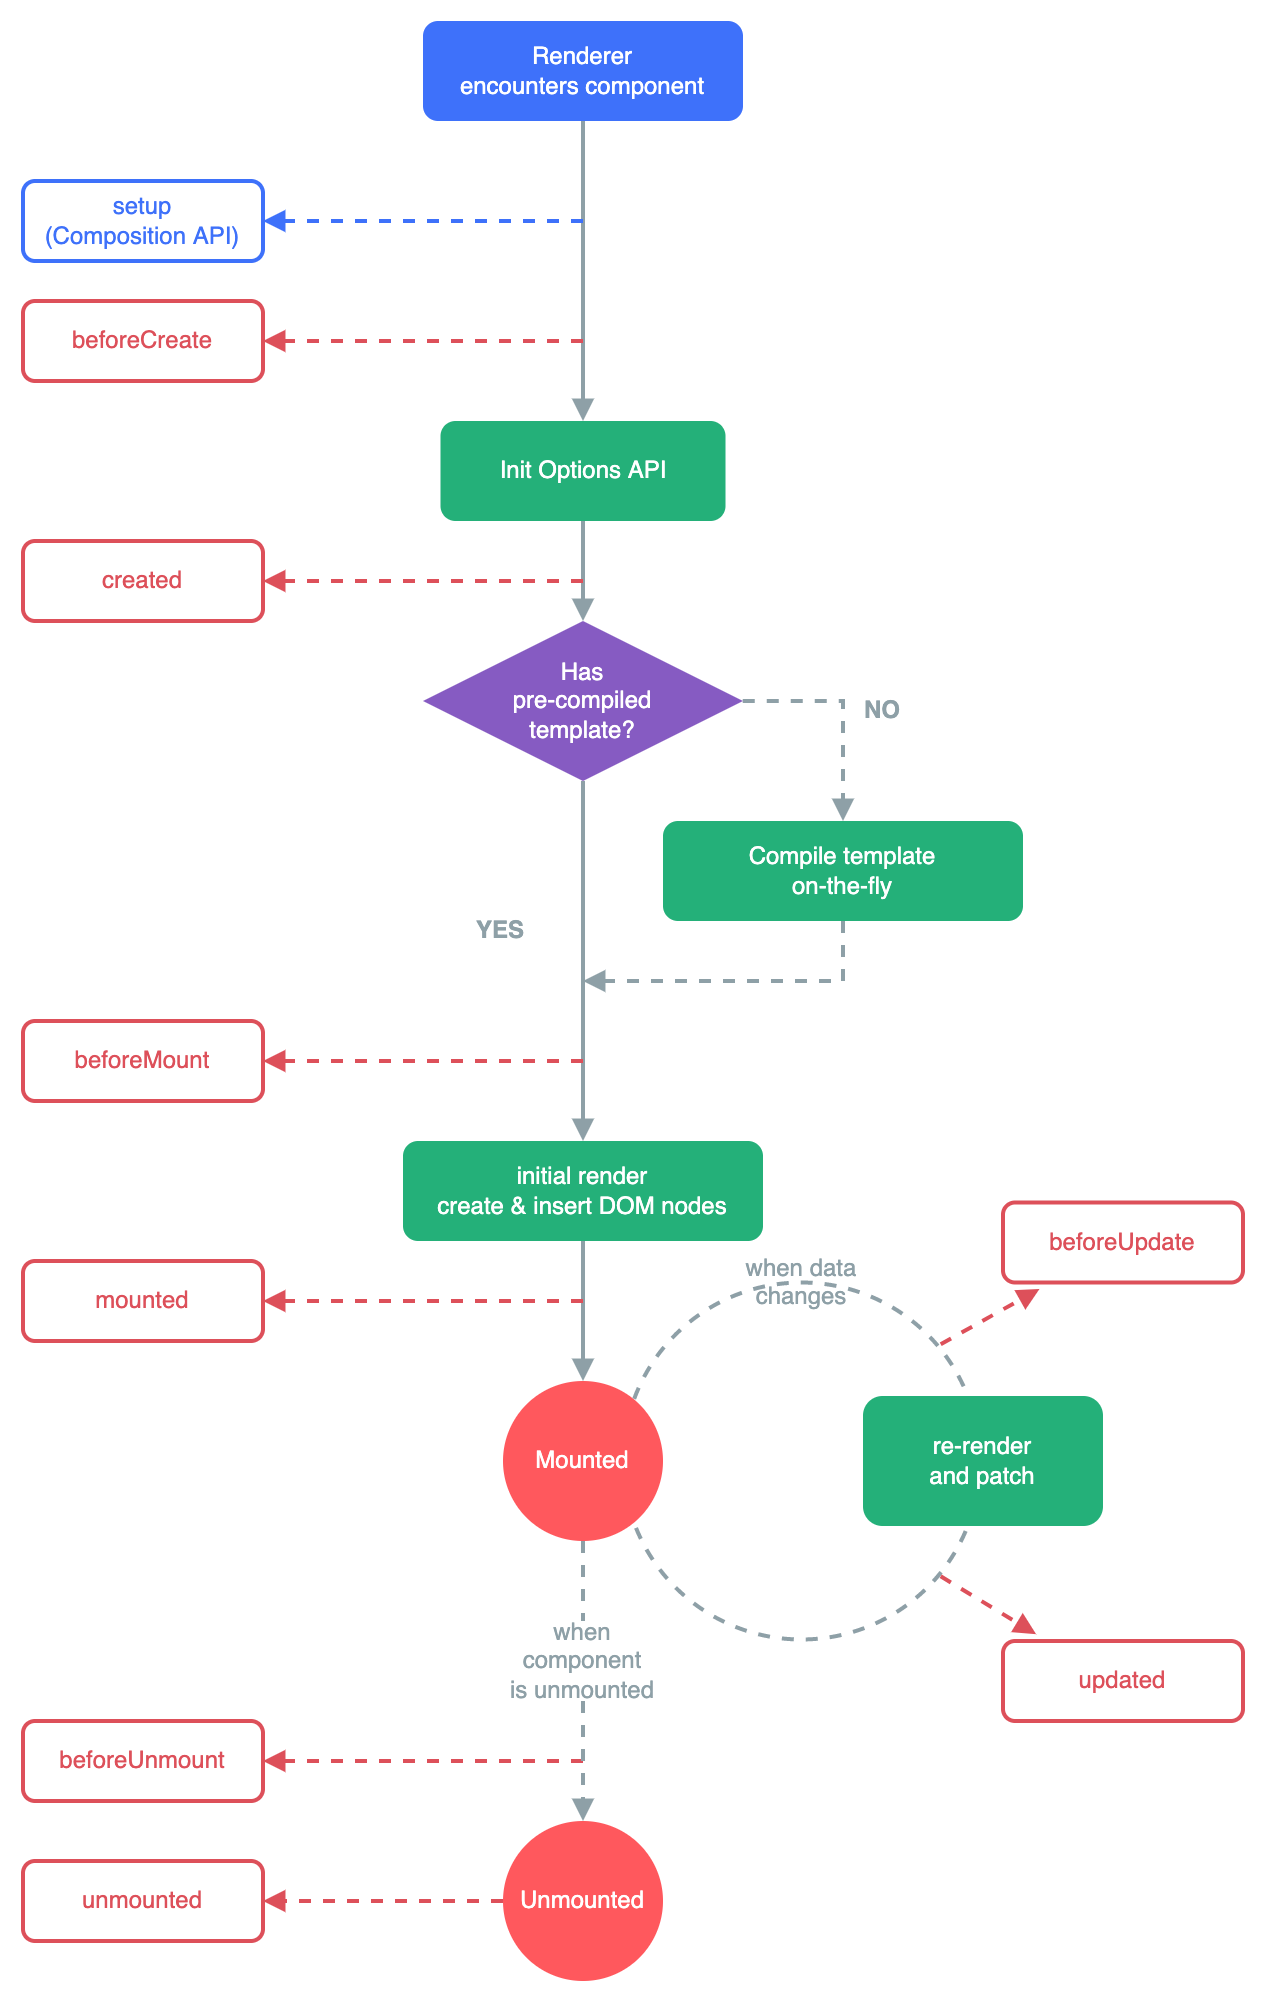
\includegraphics[scale=0.3]{./img/lifecycle.16e4c08e.png} 
\end{center}

\columnratio{0.55}
\begin{paracol}{2}
\switchcolumn[0]*%%%%%%%
Consult the
\href{https://vuejs.org/api/composition-api-lifecycle.html}{Lifecycle
Hooks API reference} for details on all lifecycle hooks and their
respective use cases.
\switchcolumn
有关所有生命周期钩子及其各自用例的详细信息,请参考\href{https://cn.vuejs.org/api/composition-api-lifecycle.html}{生命周期钩子
API 索引}。
\end{paracol}



% \columnratio{0.55}
\begin{paracol}{2}
\switchcolumn[0]*%%%%%%%
\section{Watchers}
\switchcolumn
\section{侦听器}
\switchcolumn[0]*%%%%%%%
\subsection{Basic Example}
\switchcolumn
\subsection{基本示例}
\switchcolumn[0]*%%%%%%%
Computed properties allow us to declaratively compute derived values.
However, there are cases where we need to perform "side effects" in
reaction to state changes - for example, mutating the DOM, or changing
another piece of state based on the result of an async operation.
\switchcolumn
计算属性允许我们声明性地计算衍生值。然而在有些情况下,我们需要在状态变化时执行一些``副作用'':例如更改
DOM,或是根据异步操作的结果去修改另一处的状态。

\switchcolumn[0]*%%%%%%%
With Composition API, we can use the
\href{https://vuejs.org/api/reactivity-core.html\#watch}{\texttt{watch}
function} to trigger a callback whenever a piece of reactive state
changes:
\switchcolumn
在组合式 API 中,我们可以使用
\href{https://cn.vuejs.org/api/reactivity-core.html\#watch}{\texttt{watch}
函数}在每次响应式状态发生变化时触发回调函数:
\switchcolumn[0]*%%%%%%%
\begin{codeHtml}
<script setup>
import { ref, watch } from 'vue'
//
const question = ref('')
const answer = ref('Questions usually contain a question mark. ;-)')
//
// 可以直接侦听一个 ref
watch(question, async (newQuestion, oldQuestion) => {
  if (newQuestion.indexOf('?') > -1) {
    answer.value = 'Thinking...'
    try {
      const res = await fetch('https://yesno.wtf/api')
      answer.value = (await res.json()).answer
    } catch (error) {
      answer.value = 'Error! Could not reach the API. ' + error
    }
  }
})
</script>
//
<template>
  <p>
    Ask a yes/no question:
    <input v-model="question" />
  </p>
  <p>{{ answer }}</p>
</template>
\end{codeHtml}
\switchcolumn
\begin{codeHtml}
<script setup>
import { ref, watch } from 'vue'
//
const question = ref('')
const answer = ref('Questions usually contain a question mark. ;-)')
//
// 可以直接侦听一个 ref
watch(question, async (newQuestion, oldQuestion) => {
  if (newQuestion.indexOf('?') > -1) {
    answer.value = 'Thinking...'
    try {
      const res = await fetch('https://yesno.wtf/api')
      answer.value = (await res.json()).answer
    } catch (error) {
      answer.value = 'Error! Could not reach the API. ' + error
    }
  }
})
</script>
//
<template>
  <p>
    Ask a yes/no question:
    <input v-model="question" />
  </p>
  <p>{{ answer }}</p>
</template>
\end{codeHtml}
\switchcolumn[0]*%%%%%%%
\href{https://play.vuejs.org/\#eNp9U8Fy0zAQ/ZVFF9tDah96C2mZ0umhHKBAj7oIe52oUSQjyXEyGf87KytyoDC9JPa+p+e3b1cndtd15b5HtmQrV1vZeXDo++6Wa7nrjPVwAovtAgbh6w2M0Fqzg4xOZFxzXRvtPPzq0XlpNNwEbp5lRUKEdgPaVP925jnoXS+UOgKxvJAaxEVjJ+y2hA9XxUVFGdFIvT7LtEI5JIzrqjrbGozdOmikxdqTKqmIQOV6gvOkvQDhjrqGXOOQvCzAqCa9FHBzCyeuAWT7F6uUulZ9gy7PPmZFETmQjJV7oXoke972GJHY+Axkzxupt4FalhRcYHh7TDIQcqA+LTriikFIDy0G59nG+84tq+qITpty8G0lOhmSiedefSaPZ0mnfHFG50VRRkbkj1BPceVorbFzF/+6fQj4O7g3vWpAm6Ao6JzfINw9PZaQwXuYNJJuK/U0z1nxdTLT0M7s8Ec/I3WxquLS0brRi8ddp4RHegNYhR0M/Du3pXFSAJU285osI7aSuus97K92pkF1w1nCOYNlI534qbCh8tkOVasoXkV1+sjplLZ0HGN5Vc1G2IJ5R8Np5XpKlK7J1CJntdl1UqH92k0bzdkyNc8ZRWGGz1MtbMQi1esN1tv/1F/cIdQ4e6LJod0jZzPmhV2jj/DDjy94oOcZpK57Rew3wO/ojOpjJIH2qdcN2f6DN7l9nC47RfTsHg4etUtNpZUeJz5ndPPv32j9Yve6vE6DZuNvu1R2Tg==}{Try
it in the Playground}
\switchcolumn
\href{https://play.vuejs.org/\#eNplkkGPmzAQhf/KKxdA3Rj1mpJUUdVDT22lHrlYxDRuYOzaJjRC/PcdxyGr3b2A7PfmmzcMc3awVlxGlW2z2rdO2wCvwmj3DenBGhcww6nuCZMM7QkLOmcG5FyRN9RQa8gH/BuVD9oQdtFb5Hm5KpL8pNx6/+vu8xj9KPv+CnYFqQnyhTFIdxb4vCkjpaFb32JVnyD9lVoUpKaVVmK3x9wQoLtXgtB0VP9/cOMveYk9Np/K5MM9l7jIflScLv990nTW9EcIwXNFR3DX1YwYk4dxyrNXTlIHdCrGyk8hWL+tqqvyZMQUukpaHYOnujdtilTLHPHXGyrKUiRH8i9obx+5UM4Z98j6Pu23qH/AVzP2R5CJRMl14aRw+PldIMdH3Bh3bnzxY+FcdZW2zPvlQ1CD7WVQfALquPToP/gzL4RHqsg89rJNWq3JjgGXzWCOqt812ao3GaqEqRKHcfO8/gDLkq7r6tEyW54Bf5TTlg==}{在演练场中尝试一下}


\switchcolumn[0]*%%%%%%%
\subsubsection{Watch Source Types}
\switchcolumn
\subsubsection{侦听数据源类型}
\switchcolumn[0]*%%%%%%%
\texttt{watch}'s first argument can be different types of reactive
"sources": it can be a ref (including computed refs), a reactive object,
a getter function, or an array of multiple sources:
\switchcolumn
\texttt{watch} 的第一个参数可以是不同形式的``数据源'':它可以是一个 ref
(包括计算属性)、一个响应式对象、一个 getter
函数、或多个数据源组成的数组:
\switchcolumn[0]*%%%%%%%
\begin{codeJs}
const x = ref(0)
const y = ref(0)
//
// 单个 ref
watch(x, (newX) => {
  console.log(`x is ${newX}`)
})
//
// getter 函数
watch(
  () => x.value + y.value,
  (sum) => {
    console.log(`sum of x + y is: ${sum}`)
  }
)
//
// 多个来源组成的数组
watch([x, () => y.value], ([newX, newY]) => {
  console.log(`x is ${newX} and y is ${newY}`)
})
\end{codeJs}
\switchcolumn
\begin{codeJs}
const x = ref(0)
const y = ref(0)
//
// 单个 ref
watch(x, (newX) => {
  console.log(`x is ${newX}`)
})
//
// getter 函数
watch(
  () => x.value + y.value,
  (sum) => {
    console.log(`sum of x + y is: ${sum}`)
  }
)
//
// 多个来源组成的数组
watch([x, () => y.value], ([newX, newY]) => {
  console.log(`x is ${newX} and y is ${newY}`)
})
\end{codeJs}


\switchcolumn[0]*%%%%%%%
Do note that you can't watch a property of a reactive object like this:
\switchcolumn
注意,你不能直接侦听响应式对象的属性值,例如:
\switchcolumn[0]*%%%%%%%
\begin{codeJs}
const obj = reactive({ count: 0 })
//
// 错误,因为 watch() 得到的参数是一个 number
watch(obj.count, (count) => {
  console.log(`count is: ${count}`)
})
\end{codeJs}
\switchcolumn
\begin{codeJs}
const obj = reactive({ count: 0 })
//
// 错误,因为 watch() 得到的参数是一个 number
watch(obj.count, (count) => {
  console.log(`count is: ${count}`)
})
\end{codeJs}
\switchcolumn[0]*%%%%%%%
Instead, use a getter:
\switchcolumn
这里需要用一个返回该属性的 getter 函数:


\switchcolumn[0]*%%%%%%%
\begin{codeJs}
// 提供一个 getter 函数
watch(
  () => obj.count,
  (count) => {
    console.log(`count is: ${count}`)
  }
)
\end{codeJs}
\switchcolumn
\begin{codeJs}
// 提供一个 getter 函数
watch(
  () => obj.count,
  (count) => {
    console.log(`count is: ${count}`)
  }
)
\end{codeJs}
\end{paracol}

\columnratio{0.55}
\begin{paracol}{2}

\switchcolumn[0]*%%%%%%%
\subsection{Deep Watchers}
\switchcolumn
\subsection{深层侦听器}
\switchcolumn[0]*%%%%%%%
When you call \texttt{watch()} directly on a reactive object, it will
implicitly create a deep watcher - the callback will be triggered on all
nested mutations:
\switchcolumn
直接给 \texttt{watch()}
传入一个响应式对象,会隐式地创建一个深层侦听器------该回调函数在所有嵌套的变更时都会被触发:
\switchcolumn[0]*%%%%%%%
\begin{codeJs}
const obj = reactive({ count: 0 })
//
watch(obj, (newValue, oldValue) => {
    // 在嵌套的属性变更时触发
    // 注意:`newValue` 此处和 `oldValue` 是相等的
    // 因为它们是同一个对象!
})
//
obj.count++
\end{codeJs}
\switchcolumn
\begin{codeJs}
const obj = reactive({ count: 0 })
//
watch(obj, (newValue, oldValue) => {
    // 在嵌套的属性变更时触发
    // 注意:`newValue` 此处和 `oldValue` 是相等的
    // 因为它们是同一个对象!
})
//
obj.count++
\end{codeJs}


\switchcolumn[0]*%%%%%%%
This should be differentiated with a getter that returns a reactive
object - in the latter case, the callback will only fire if the getter
returns a different object:
\switchcolumn
相比之下,一个返回响应式对象的 getter
函数,只有在返回不同的对象时,才会触发回调:
\switchcolumn[0]*%%%%%%%
\begin{codeJs}
watch(
  () => state.someObject,
  () => {
    // 仅当 state.someObject 被替换时触发
  }
)
\end{codeJs}
\switchcolumn
\begin{codeJs}
watch(
  () => state.someObject,
  () => {
    // 仅当 state.someObject 被替换时触发
  }
)
\end{codeJs}
\switchcolumn[0]*%%%%%%%
You can, however, force the second case into a deep watcher by
explicitly using the \texttt{deep} option:
\switchcolumn
你也可以给上面这个例子显式地加上 \texttt{deep}
选项,强制转成深层侦听器:


\switchcolumn[0]*%%%%%%%
\begin{codeJs}
watch(
  () => state.someObject,
  (newValue, oldValue) => {
    // 注意:`newValue` 此处和 `oldValue` 是相等的
    // *除非* state.someObject 被整个替换了
  },
  { deep: true }
)
\end{codeJs}
\switchcolumn
\begin{codeJs}
watch(
  () => state.someObject,
  (newValue, oldValue) => {
    // 注意:`newValue` 此处和 `oldValue` 是相等的
    // *除非* state.someObject 被整个替换了
  },
  { deep: true }
)
\end{codeJs}
\switchcolumn[0]*%%%%%%%
\begin{vueQuoteWarn}{Use with Caution}
Deep watch requires traversing all nested properties in the watched
object, and can be expensive when used on large data structures. Use it
only when necessary and beware of the performance implications.
\end{vueQuoteWarn}
\switchcolumn
\begin{vueQuoteWarn}{谨慎使用}
深度侦听需要遍历被侦听对象中的所有嵌套的属性,当用于大型数据结构时,开销很大。因此请只在必要时才使用它,并且要留意性能。
\end{vueQuoteWarn}
\end{paracol}

\columnratio{0.55}
\begin{paracol}{2}

\switchcolumn[0]*%%%%%%%
\subsection{Eager Watchers}
\switchcolumn
\subsection{即时回调的侦听器}
\switchcolumn[0]*%%%%%%%
\texttt{watch} is lazy by default: the callback won't be called until
the watched source has changed. But in some cases we may want the same
callback logic to be run eagerly - for example, we may want to fetch
some initial data, and then re-fetch the data whenever relevant state
changes.
\switchcolumn
\texttt{watch}
默认是懒执行的:仅当数据源变化时,才会执行回调。但在某些场景中,我们希望在创建侦听器时,立即执行一遍回调。举例来说,我们想请求一些初始数据,然后在相关状态更改时重新请求数据。
\switchcolumn[0]*%%%%%%%
We can force a watcher's callback to be executed immediately by passing
the \texttt{immediate:\ true} option:
\switchcolumn
我们可以通过传入 \texttt{immediate:\ true}
选项来强制侦听器的回调立即执行:
\switchcolumn[0]*%%%%%%%
\begin{codeJs}
watch(source, (newValue, oldValue) => {
    // 立即执行,且当 `source` 改变时再次执行
}, { immediate: true })
\end{codeJs}
\switchcolumn
\begin{codeJs}
watch(source, (newValue, oldValue) => {
    // 立即执行,且当 `source` 改变时再次执行
}, { immediate: true })
\end{codeJs}
\switchcolumn[0]*%%%%%%%
\subsection{watchEffect()}
\switchcolumn
\subsection{watchEffect()}



\switchcolumn[0]*%%%%%%%
It is common for the watcher callback to use exactly the same reactive
state as the source. For example, consider the following code, which
uses a watcher to load a remote resource whenever the \texttt{todoId}
ref changes:
\switchcolumn
侦听器的回调使用与源完全相同的响应式状态是很常见的。例如下面的代码,在每当
\texttt{todoId} 的引用发生变化时使用侦听器来加载一个远程资源:
\switchcolumn[0]*%%%%%%%
\begin{codeJs}
const todoId = ref(1)
const data = ref(null)
//
watch(todoId, async () => {
  const response = await fetch(
    `https://jsonplaceholder.typicode.com/todos/${todoId.value}`
  )
  data.value = await response.json()
}, { immediate: true })
\end{codeJs}
\switchcolumn
\begin{codeJs}
const todoId = ref(1)
const data = ref(null)
//
watch(todoId, async () => {
  const response = await fetch(
    `https://jsonplaceholder.typicode.com/todos/${todoId.value}`
  )
  data.value = await response.json()
}, { immediate: true })
\end{codeJs}
\switchcolumn[0]*%%%%%%%
In particular, notice how the watcher uses \texttt{todoId} twice, once
as the source and then again inside the callback.
\switchcolumn
特别是注意侦听器是如何两次使用 \texttt{todoId}
的,一次是作为源,另一次是在回调中。
\switchcolumn[0]*%%%%%%%
This can be simplified with
\href{https://vuejs.org/api/reactivity-core.html\#watcheffect}{\texttt{watchEffect()}}.
\texttt{watchEffect()} allows us to track the callback's reactive
dependencies automatically. The watcher above can be rewritten as:
\switchcolumn
我们可以用
\href{https://cn.vuejs.org/api/reactivity-core.html\#watcheffect}{\texttt{watchEffect}
函数} 来简化上面的代码。\texttt{watchEffect()}
允许我们自动跟踪回调的响应式依赖。上面的侦听器可以重写为:
\switchcolumn[0]*%%%%%%%
\begin{codeJs}
watchEffect(async () => {
  const response = await fetch(
    `https://jsonplaceholder.typicode.com/todos/${todoId.value}`
  )
  data.value = await response.json()
})
\end{codeJs}
\switchcolumn
\begin{codeJs}
watchEffect(async () => {
  const response = await fetch(
    `https://jsonplaceholder.typicode.com/todos/${todoId.value}`
  )
  data.value = await response.json()
})
\end{codeJs}


\switchcolumn[0]*%%%%%%%
Here, the callback will run immediately, there's no need to specify
\texttt{immediate:\ true}. During its execution, it will automatically
track \texttt{todoId.value} as a dependency (similar to computed
properties). Whenever \texttt{todoId.value} changes, the callback will
be run again. With \texttt{watchEffect()}, we no longer need to pass
\texttt{todoId} explicitly as the source value.
\switchcolumn
这个例子中,回调会立即执行,不需要指定
\texttt{immediate:\ true}。在执行期间,它会自动追踪
\texttt{todoId.value} 作为依赖(和计算属性类似)。每当
\texttt{todoId.value} 变化时,回调会再次执行。有了
\texttt{watchEffect()},我们不再需要明确传递 \texttt{todoId} 作为源值。
\switchcolumn[0]*%%%%%%%
You can check out \href{https://vuejs.org/examples/\#fetching-data}{this
example} of \texttt{watchEffect()} and reactive data-fetching in action.
\switchcolumn
你可以参考一下\href{https://cn.vuejs.org/examples/\#fetching-data}{这个例子}的
\texttt{watchEffect} 和响应式的数据请求的操作。
\switchcolumn[0]*%%%%%%%
For examples like these, with only one dependency, the benefit of
\texttt{watchEffect()} is relatively small. But for watchers that have
multiple dependencies, using \texttt{watchEffect()} removes the burden
of having to maintain the list of dependencies manually. In addition, if
you need to watch several properties in a nested data structure,
\texttt{watchEffect()} may prove more efficient than a deep watcher, as
it will only track the properties that are used in the callback, rather
than recursively tracking all of them.
\switchcolumn
对于这种只有一个依赖项的例子来说,\texttt{watchEffect()}
的好处相对较小。但是对于有多个依赖项的侦听器来说,使用
\texttt{watchEffect()}
可以消除手动维护依赖列表的负担。此外,如果你需要侦听一个嵌套数据结构中的几个属性,\texttt{watchEffect()}
可能会比深度侦听器更有效,因为它将只跟踪回调中被使用到的属性,而不是递归地跟踪所有的属性。
\switchcolumn[0]*%%%%%%%
\begin{vueQuote}{TIP}
\texttt{watchEffect} only tracks dependencies during its
\textbf{synchronous} execution. When using it with an async callback,
only properties accessed before the first \texttt{await} tick will be
tracked.
\end{vueQuote}
\switchcolumn
\begin{vueQuote}{TIP}
\texttt{watchEffect}
仅会在其\textbf{同步}执行期间,才追踪依赖。在使用异步回调时,只有在第一个
\texttt{await} 正常工作前访问到的属性才会被追踪。
\end{vueQuote}
\end{paracol}

\columnratio{0.55}
\begin{paracol}{2}

\switchcolumn[0]*%%%%%%%
\subsubsection{watch vs. watchEffect}
\switchcolumn
\subsubsection{watch vs. watchEffect}
\switchcolumn[0]*%%%%%%%
\texttt{watch} and \texttt{watchEffect} both allow us to reactively
perform side effects. Their main difference is the way they track their
reactive dependencies:
\switchcolumn
\texttt{watch} 和 \texttt{watchEffect}
都能响应式地执行有副作用的回调。它们之间的主要区别是追踪响应式依赖的方式:
\switchcolumn[0]*%%%%%%%
\begin{itemize}
\item
    \texttt{watch} only tracks the explicitly watched source. It won't
    track anything accessed inside the callback. In addition, the callback
    only triggers when the source has actually changed. \texttt{watch}
    separates dependency tracking from the side effect, giving us more
    precise control over when the callback should fire.
\item
    \texttt{watchEffect}, on the other hand, combines dependency tracking
    and side effect into one phase. It automatically tracks every reactive
    property accessed during its synchronous execution. This is more
    convenient and typically results in terser code, but makes its
    reactive dependencies less explicit.
\end{itemize}
\switchcolumn
\begin{itemize}
\item
    \texttt{watch}
    只追踪明确侦听的数据源。它不会追踪任何在回调中访问到的东西。另外,仅在数据源确实改变时才会触发回调。\texttt{watch}
    会避免在发生副作用时追踪依赖,因此,我们能更加精确地控制回调函数的触发时机。
\item
    \texttt{watchEffect},则会在副作用发生期间追踪依赖。它会在同步执行过程中,自动追踪所有能访问到的响应式属性。这更方便,而且代码往往更简洁,但有时其响应性依赖关系会不那么明确。
\end{itemize}
\switchcolumn[0]*%%%%%%%
\subsection{Callback Flush Timing}
\switchcolumn
\subsection{回调的触发时机}


\switchcolumn[0]*%%%%%%%
When you mutate reactive state, it may trigger both Vue component
updates and watcher callbacks created by you.
\switchcolumn
当你更改了响应式状态,它可能会同时触发 Vue 组件更新和侦听器回调。
\switchcolumn[0]*%%%%%%%
By default, user-created watcher callbacks are called \textbf{before}
Vue component updates. This means if you attempt to access the DOM
inside a watcher callback, the DOM will be in the state before Vue has
applied any updates.
\switchcolumn
默认情况下,用户创建的侦听器回调,都会在 Vue
组件更新\textbf{之前}被调用。这意味着你在侦听器回调中访问的 DOM 将是被
Vue 更新之前的状态。
\switchcolumn[0]*%%%%%%%
If you want to access the DOM in a watcher callback \textbf{after} Vue
has updated it, you need to specify the
\texttt{flush:\ \textquotesingle{}post\textquotesingle{}} option:
\switchcolumn
如果想在侦听器回调中能访问被 Vue 更新\textbf{之后}的 DOM,你需要指明
\texttt{flush:\ \textquotesingle{}post\textquotesingle{}} 选项:
\switchcolumn[0]*%%%%%%%
\begin{codeJs}
watch(source, callback, {
  flush: 'post'
})
//
watchEffect(callback, {
  flush: 'post'
})
\end{codeJs}
\switchcolumn
\begin{codeJs}
watch(source, callback, {
  flush: 'post'
})
//
watchEffect(callback, {
  flush: 'post'
})
\end{codeJs}


\switchcolumn[0]*%%%%%%%
Post-flush \texttt{watchEffect()} also has a convenience alias,
\texttt{watchPostEffect()}:
\switchcolumn
后置刷新的 \texttt{watchEffect()} 有个更方便的别名
\texttt{watchPostEffect()}:
\switchcolumn[0]*%%%%%%%
\begin{codeJs}
import { watchPostEffect } from 'vue'
//
watchPostEffect(() => {
  /* 在 Vue 更新后执行 */
})
\end{codeJs}
\switchcolumn
\begin{codeJs}
import { watchPostEffect } from 'vue'
//
watchPostEffect(() => {
  /* 在 Vue 更新后执行 */
})
\end{codeJs}
\end{paracol}

\columnratio{0.55}
\begin{paracol}{2}

\switchcolumn[0]*%%%%%%%
\subsection{Stopping a Watcher}
\switchcolumn
\subsection{停止侦听器}
\switchcolumn[0]*%%%%%%%
Watchers declared synchronously inside \texttt{setup()} or
\texttt{\textless{}script\ setup\textgreater{}} are bound to the owner
component instance, and will be automatically stopped when the owner
component is unmounted. In most cases, you don't need to worry about
stopping the watcher yourself.
\switchcolumn
在 \texttt{setup()} 或 \texttt{\textless{}script\ setup\textgreater{}}
中用同步语句创建的侦听器,会自动绑定到宿主组件实例上,并且会在宿主组件卸载时自动停止。因此,在大多数情况下,你无需关心怎么停止一个侦听器。
\switchcolumn[0]*%%%%%%%
The key here is that the watcher must be created \textbf{synchronously}:
if the watcher is created in an async callback, it won't be bound to the
owner component and must be stopped manually to avoid memory leaks.
Here's an example:
\switchcolumn
一个关键点是,侦听器必须用\textbf{同步}语句创建:如果用异步回调创建一个侦听器,那么它不会绑定到当前组件上,你必须手动停止它,以防内存泄漏。如下方这个例子:
\switchcolumn[0]*%%%%%%%
\begin{codeHtml}
<script setup>
import { watchEffect } from 'vue'
//
// 它会自动停止
watchEffect(() => {})
//
// ...这个则不会!
setTimeout(() => {
    watchEffect(() => {})
}, 100)
</script>
\end{codeHtml}
\switchcolumn
\begin{codeHtml}
<script setup>
import { watchEffect } from 'vue'
//
// 它会自动停止
watchEffect(() => {})
//
// ...这个则不会!
setTimeout(() => {
    watchEffect(() => {})
}, 100)
</script>
\end{codeHtml}
\switchcolumn[0]*%%%%%%%
To manually stop a watcher, use the returned handle function. This works
for both \texttt{watch} and \texttt{watchEffect}:
\switchcolumn
要手动停止一个侦听器,请调用 \texttt{watch} 或 \texttt{watchEffect}
返回的函数:


\switchcolumn[0]*%%%%%%%
\begin{codeJs}
const unwatch = watchEffect(() => {})
//
// ...当该侦听器不再需要时
unwatch()
\end{codeJs}
\switchcolumn
\begin{codeJs}
const unwatch = watchEffect(() => {})
//
// ...当该侦听器不再需要时
unwatch()
\end{codeJs}
\switchcolumn[0]*%%%%%%%
Note that there should be very few cases where you need to create
watchers asynchronously, and synchronous creation should be preferred
whenever possible. If you need to wait for some async data, you can make
your watch logic conditional instead:
\switchcolumn
注意,需要异步创建侦听器的情况很少,请尽可能选择同步创建。如果需要等待一些异步数据,你可以使用条件式的侦听逻辑:
\switchcolumn[0]*%%%%%%%
\begin{codeJs}
// 需要异步请求得到的数据
const data = ref(null)
//
watchEffect(() => {
  if (data.value) {
    // 数据加载后执行某些操作...
  }
})
\end{codeJs}
\switchcolumn
\begin{codeJs}
// 需要异步请求得到的数据
const data = ref(null)
//
watchEffect(() => {
  if (data.value) {
    // 数据加载后执行某些操作...
  }
})
\end{codeJs}
\end{paracol}


% \columnratio{0.55}
\begin{paracol}{2}

\switchcolumn[0]*%%%%%%%
\section{Template Refs}
\switchcolumn
\section{模板引用}
\switchcolumn[0]*%%%%%%%
While Vue's declarative rendering model abstracts away most of the
direct DOM operations for you, there may still be cases where we need
direct access to the underlying DOM elements. To achieve this, we can
use the special \texttt{ref} attribute:
\switchcolumn
虽然 Vue 的声明性渲染模型为你抽象了大部分对 DOM
的直接操作,但在某些情况下,我们仍然需要直接访问底层 DOM
元素。要实现这一点,我们可以使用特殊的 \texttt{ref} attribute:
\switchcolumn[0]*%%%%%%%
\begin{codeHtml}
<input ref="input">
\end{codeHtml}
\switchcolumn
\begin{codeHtml}
<input ref="input">
\end{codeHtml}

\switchcolumn[0]*%%%%%%%
\texttt{ref} is a special attribute, similar to the \texttt{key}
attribute discussed in the \texttt{v-for} chapter. It allows us to
obtain a direct reference to a specific DOM element or child component
instance after it's mounted. This may be useful when you want to, for
example, programmatically focus an input on component mount, or
initialize a 3rd party library on an element.
\switchcolumn
\texttt{ref} 是一个特殊的 attribute,和 \texttt{v-for} 章节中提到的
\texttt{key} 类似。它允许我们在一个特定的 DOM
元素或子组件实例被挂载后,获得对它的直接引用。这可能很有用,比如说在组件挂载时将焦点设置到一个
input 元素上,或在一个元素上初始化一个第三方库。


\switchcolumn[0]*%%%%%%%
\subsection{Accessing the Refs}
\switchcolumn
\subsection{访问模板引用}
\switchcolumn[0]*%%%%%%%
To obtain the reference with Composition API, we need to declare a ref
with the same name:
\switchcolumn
为了通过组合式 API 获得该模板引用,我们需要声明一个同名的 ref:
\switchcolumn[0]*%%%%%%%
\begin{codeHtml}
<script setup>
import { ref, onMounted } from 'vue'
//
// 声明一个 ref 来存放该元素的引用
// 必须和模板里的 ref 同名
const input = ref(null)
//
onMounted(() => {
  input.value.focus()
})
</script>
//
<template>
  <input ref="input" />
</template>
\end{codeHtml}
\switchcolumn
\begin{codeHtml}
<script setup>
import { ref, onMounted } from 'vue'
//
// 声明一个 ref 来存放该元素的引用
// 必须和模板里的 ref 同名
const input = ref(null)
//
onMounted(() => {
  input.value.focus()
})
</script>
//
<template>
  <input ref="input" />
</template>
\end{codeHtml}


\switchcolumn[0]*%%%%%%%
If not using \texttt{\textless{}script\ setup\textgreater{}}, make sure
to also return the ref from \texttt{setup()}:
\switchcolumn
如果不使用 \texttt{\textless{}script\ setup\textgreater{}},需确保从
\texttt{setup()} 返回 ref:
\switchcolumn[0]*%%%%%%%
\begin{codeJs}
export default {
  setup() {
    const input = ref(null)
    // ...
    return {
      input
    }
  }
}
\end{codeJs}
\switchcolumn
\begin{codeJs}
export default {
  setup() {
    const input = ref(null)
    // ...
    return {
      input
    }
  }
}
\end{codeJs}
\switchcolumn[0]*%%%%%%%
Note that you can only access the ref \textbf{after the component is
mounted.} If you try to access \texttt{input} in a template expression,
it will be \texttt{null} on the first render. This is because the
element doesn't exist until after the first render!
\switchcolumn
注意,你只可以\textbf{在组件挂载后}才能访问模板引用。如果你想在模板中的表达式上访问
\texttt{input},在初次渲染时会是
\texttt{null}。这是因为在初次渲染前这个元素还不存在呢!


\switchcolumn[0]*%%%%%%%
If you are trying to watch the changes of a template ref, make sure to
account for the case where the ref has \texttt{null} value:
\switchcolumn
如果你需要侦听一个模板引用 ref 的变化,确保考虑到其值为 \texttt{null}
的情况:
\switchcolumn[0]*%%%%%%%
\begin{codeJs}
watchEffect(() => {
  if (input.value) {
    input.value.focus()
  } else {
    // 此时还未挂载,或此元素已经被卸载(例如通过 v-if 控制)
  }
})
\end{codeJs}
\switchcolumn
\begin{codeJs}
watchEffect(() => {
  if (input.value) {
    input.value.focus()
  } else {
    // 此时还未挂载,或此元素已经被卸载(例如通过 v-if 控制)
  }
})
\end{codeJs}
\switchcolumn[0]*%%%%%%%
See also:
\href{https://vuejs.org/guide/typescript/composition-api.html\#typing-template-refs}{Typing
Template Refs}
\switchcolumn
也可参考:\href{https://cn.vuejs.org/guide/typescript/composition-api.html\#typing-template-refs}{为模板引用标注类型}


\switchcolumn[0]*%%%%%%%
\subsection{Refs inside v-for}
\switchcolumn
\subsection{v-for 中的模板引用}
\switchcolumn[0]*%%%%%%%
\begin{quote}
Requires v3.2.25 or above
\end{quote}
\switchcolumn
\begin{quote}
需要 v3.2.25 及以上版本
\end{quote}
\switchcolumn[0]*%%%%%%%
When \texttt{ref} is used inside \texttt{v-for}, the corresponding ref
should contain an Array value, which will be populated with the elements
after mount:
\switchcolumn
当在 \texttt{v-for} 中使用模板引用时,对应的 ref
中包含的值是一个数组,它将在元素被挂载后包含对应整个列表的所有元素:


\switchcolumn[0]*%%%%%%%
\begin{codeHtml}
<script setup>
import { ref, onMounted } from 'vue'
//
const list = ref([
  /* ... */
])
//
const itemRefs = ref([])
//
onMounted(() => console.log(itemRefs.value))
</script>
<!-- -->
<template>
  <ul>
    <li v-for="item in list" ref="itemRefs">
      {{ item }}
    </li>
  </ul>
</template>
\end{codeHtml}
\switchcolumn
\begin{codeHtml}
<script setup>
import { ref, onMounted } from 'vue'
//
const list = ref([
  /* ... */
])
//
const itemRefs = ref([])
//
onMounted(() => console.log(itemRefs.value))
</script>
<!-- -->
<template>
  <ul>
    <li v-for="item in list" ref="itemRefs">
      {{ item }}
    </li>
  </ul>
</template>
\end{codeHtml}
\switchcolumn[0]*%%%%%%%
\href{https://play.vuejs.org/\#eNpFjs1qwzAQhF9l0CU2uDZtb8UOlJ576bXqwaQyCGRJyCsTEHr3rGwnOehnd2e+nSQ+vW/XqMSH6JdL0J6wKIr+LK2evQuEhKCmBs5+u2hJ/SNjCm7GiV0naaW9OLsQjOZrKNrq97XBW4P3v/o51qTmHzUtd8k+e0CrqsZwRpIWGI0KVN0N7TqaqNp59JUuEt2SutKXY5elmimZT9/t2Tk1F+z0ZiTFFdBHs738Mxrry+TCIEWhQ9sttRQl0tEsK6U4HEBKW3LkfDA6o3dst3H77rFM5BtTfm/P}{Try
it in the Playground}
\switchcolumn
\href{https://play.vuejs.org/\#eNpFjs1qwzAQhF9l0CU2uDZtb8UOlJ576bXqwaQyCGRJyCsTEHr3rGwnOehnd2e+nSQ+vW/XqMSH6JdL0J6wKIr+LK2evQuEhKCmBs5+u2hJ/SNjCm7GiV0naaW9OLsQjOZrKNrq97XBW4P3v/o51qTmHzUtd8k+e0CrqsZwRpIWGI0KVN0N7TqaqNp59JUuEt2SutKXY5elmimZT9/t2Tk1F+z0ZiTFFdBHs738Mxrry+TCIEWhQ9sttRQl0tEsK6U4HEBKW3LkfDA6o3dst3H77rFM5BtTfm/P}{在演练场中尝试一下}
\switchcolumn[0]*%%%%%%%
It should be noted that the ref array does \textbf{not} guarantee the
same order as the source array.
\switchcolumn
应该注意的是,ref 数组\textbf{并不}保证与源数组相同的顺序。


\switchcolumn[0]*%%%%%%% 
\subsection{Function Refs}
\switchcolumn
\subsection{函数模板引用}
\switchcolumn[0]*%%%%%%%
Instead of a string key, the \texttt{ref} attribute can also be bound to
a function, which will be called on each component update and gives you
full flexibility on where to store the element reference. The function
receives the element reference as the first argument:
\switchcolumn
除了使用字符串值作名字,\texttt{ref} attribute
还可以绑定为一个函数,会在每次组件更新时都被调用。该函数会收到元素引用作为其第一个参数:
\switchcolumn[0]*%%%%%%%
\begin{codeHtml}
<input :ref="(el) => { /* 将 el 赋值给一个数据属性或 ref 变量 */ }">
\end{codeHtml}
\switchcolumn
\begin{codeHtml}
<input :ref="(el) => { /* 将 el 赋值给一个数据属性或 ref 变量 */ }">
\end{codeHtml}


\switchcolumn[0]*%%%%%%%
Note we are using a dynamic \texttt{:ref} binding so we can pass it a
function instead of a ref name string. When the element is unmounted,
the argument will be \texttt{null}. You can, of course, use a method
instead of an inline function.
\switchcolumn
注意我们这里需要使用动态的 \texttt{:ref}
绑定才能够传入一个函数。当绑定的元素被卸载时,函数也会被调用一次,此时的
\texttt{el} 参数会是
\texttt{null}。你当然也可以绑定一个组件方法而不是内联函数。
\switchcolumn[0]*%%%%%%%
\subsection{Ref on Component}
\switchcolumn
\subsection{组件上的 ref}
\switchcolumn[0]*%%%%%%%
\begin{quote}
This section assumes knowledge of
\href{https://vuejs.org/guide/essentials/component-basics.html}{Components}.
Feel free to skip it and come back later.
\end{quote}
\switchcolumn
\begin{quote}
这一小节假设你已了解\href{https://cn.vuejs.org/guide/essentials/component-basics.html}{组件}的相关知识,或者你也可以先跳过这里,之后再回来看。
\end{quote}


\switchcolumn[0]*%%%%%%%
\texttt{ref} can also be used on a child component. In this case the
reference will be that of a component instance:
\switchcolumn
模板引用也可以被用在一个子组件上。这种情况下引用中获得的值是组件实例:
\switchcolumn[0]*%%%%%%%
\begin{codeHtml}
<script setup>
import { ref, onMounted } from 'vue'
import Child from './Child.vue'
<!-- -->
const child = ref(null)
<!-- -->
onMounted(() => {
  // child.value 是 <Child /> 组件的实例
})
</script>
<!-- -->
<template>
  <Child ref="child" />
</template>
\end{codeHtml}
\switchcolumn
\begin{codeHtml}
<script setup>
import { ref, onMounted } from 'vue'
import Child from './Child.vue'
<!-- -->
const child = ref(null)
<!-- -->
onMounted(() => {
  // child.value 是 <Child /> 组件的实例
})
</script>
<!-- -->
<template>
  <Child ref="child" />
</template>
\end{codeHtml}
\switchcolumn[0]*%%%%%%%
If the child component is using Options API or not using
\texttt{\textless{}script\ setup\textgreater{}}, the referenced instance
will be identical to the child component's \texttt{this}, which means
the parent component will have full access to every property and method
of the child component. This makes it easy to create tightly coupled
implementation details between the parent and the child, so component
refs should be only used when absolutely needed - in most cases, you
should try to implement parent / child interactions using the standard
props and emit interfaces first.
\switchcolumn
如果一个子组件使用的是选项式 API 或没有使用
\texttt{\textless{}script\ setup\textgreater{}},被引用的组件实例和该子组件的
\texttt{this}
完全一致,这意味着父组件对子组件的每一个属性和方法都有完全的访问权。这使得在父组件和子组件之间创建紧密耦合的实现细节变得很容易,当然也因此,应该只在绝对需要时才使用组件引用。大多数情况下,你应该首先使用标准的
props 和 emit 接口来实现父子组件交互。


\switchcolumn[0]*%%%%%%%
An exception here is that components using
\texttt{\textless{}script\ setup\textgreater{}} are \textbf{private by
default}: a parent component referencing a child component using
\texttt{\textless{}script\ setup\textgreater{}} won't be able to access
anything unless the child component chooses to expose a public interface
using the \texttt{defineExpose} macro:
\switchcolumn
有一个例外的情况,使用了 \texttt{\textless{}script\ setup\textgreater{}}
的组件是\textbf{默认私有}的:一个父组件无法访问到一个使用了
\texttt{\textless{}script\ setup\textgreater{}}
的子组件中的任何东西,除非子组件在其中通过 \texttt{defineExpose}
宏显式暴露:
\switchcolumn[0]*%%%%%%%
\begin{codeHtml}
<script setup>
import { ref } from 'vue'
<!-- -->
const a = 1
const b = ref(2)
<!-- -->
// 像 defineExpose 这样的编译器宏不需要导入
defineExpose({
  a,
  b
})
</script>
\end{codeHtml}
\switchcolumn
\begin{codeHtml}
<script setup>
import { ref } from 'vue'
<!-- -->
const a = 1
const b = ref(2)
<!-- -->
// 像 defineExpose 这样的编译器宏不需要导入
defineExpose({
  a,
  b
})
</script>
\end{codeHtml}
\switchcolumn[0]*%%%%%%%
When a parent gets an instance of this component via template refs, the
retrieved instance will be of the shape
\texttt{\{\ a:\ number,\ b:\ number\ \}} (refs are automatically
unwrapped just like on normal instances).
\switchcolumn
当父组件通过模板引用获取到了该组件的实例时,得到的实例类型为
\texttt{\{\ a:\ number,\ b:\ number\ \}} (ref
都会自动解包,和一般的实例一样)。


\switchcolumn[0]*%%%%%%%
See also:
\href{https://vuejs.org/guide/typescript/composition-api.html\#typing-component-template-refs}{Typing
Component Template Refs}
\switchcolumn
TypeScript
用户请参考:\href{https://cn.vuejs.org/guide/typescript/composition-api.html\#typing-component-template-refs}{为组件的模板引用标注类型}
\end{paracol}
 
% \columnratio{0.55}
\begin{paracol}{2}
\switchcolumn[0]*%%%%%%%
\section{Components Basics}
\switchcolumn
\section{组件基础}
\switchcolumn[0]*%%%%%%%
Components allow us to split the UI into independent and reusable
pieces, and think about each piece in isolation. It's common for an app
to be organized into a tree of nested components:
\switchcolumn
组件允许我们将 UI
划分为独立的、可重用的部分,并且可以对每个部分进行单独的思考。在实际应用中,组件常常被组织成层层嵌套的树状结构:
\end{paracol}


\begin{center} 
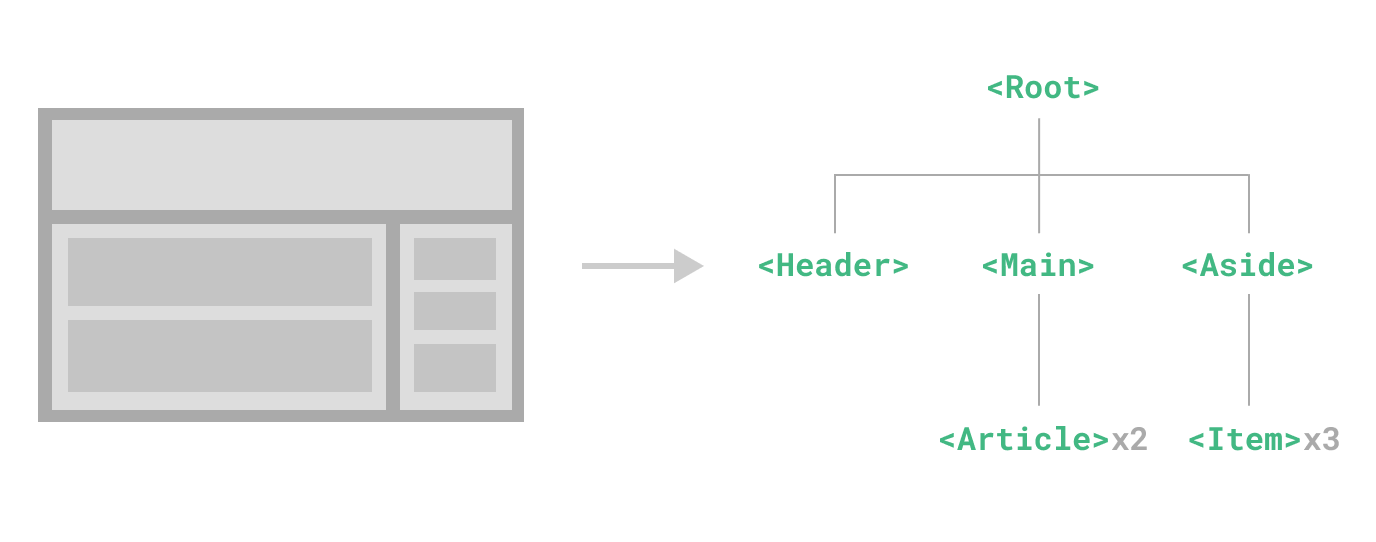
\includegraphics{./img/components.7fbb3771.png} 
\end{center}

\columnratio{0.55}
\begin{paracol}{2}

\switchcolumn[0]*%%%%%%%
This is very similar to how we nest native HTML elements, but Vue
implements its own component model that allow us to encapsulate custom
content and logic in each component. Vue also plays nicely with native
Web Components. If you are curious about the relationship between Vue
Components and native Web Components,
\href{https://vuejs.org/guide/extras/web-components.html}{read more
here}.
\switchcolumn
这和我们嵌套 HTML 元素的方式类似,Vue
实现了自己的组件模型,使我们可以在每个组件内封装自定义内容与逻辑。Vue
同样也能很好地配合原生 Web Component。如果你想知道 Vue 组件与原生 Web
Components
之间的关系,可以\href{https://cn.vuejs.org/guide/extras/web-components.html}{阅读此章节}。
\switchcolumn[0]*%%%%%%%
\subsection{Defining a Component}
\switchcolumn
\subsection{定义一个组件}
\switchcolumn[0]*%%%%%%%
When using a build step, we typically define each Vue component in a
dedicated file using the \texttt{.vue} extension - known as a
\href{https://vuejs.org/guide/scaling-up/sfc.html}{Single-File
Component} (SFC for short):
\switchcolumn
当使用构建步骤时,我们一般会将 Vue 组件定义在一个单独的 \texttt{.vue}
文件中,这被叫做\href{https://cn.vuejs.org/guide/scaling-up/sfc.html}{单文件组件}
(简称 SFC):
\switchcolumn[0]*%%%%%%%
\begin{codeHtml}
<script setup>
import { ref } from 'vue'
//
const count = ref(0)
</script>
//
<template>
    <button @click="count++">You clicked me {{ count }} times.</button>
</template>
\end{codeHtml}
\switchcolumn
\begin{codeHtml}
<script setup>
import { ref } from 'vue'
//
const count = ref(0)
</script>
//
<template>
    <button @click="count++">You clicked me {{ count }} times.</button>
</template>
\end{codeHtml}
\switchcolumn[0]*%%%%%%%
When not using a build step, a Vue component can be defined as a plain
JavaScript object containing Vue-specific options:
\switchcolumn
当不使用构建步骤时,一个 Vue 组件以一个包含 Vue 特定选项的 JavaScript
对象来定义:


\switchcolumn[0]*%%%%%%%
\begin{codeJs}
import { ref } from 'vue'
//
export default {
  setup() {
    const count = ref(0)
    return { count }
  },
  template: `
    <button @click="count++">
      You clicked me {{ count }} times.
    </button>`
  // 也可以针对一个 DOM 内联模板:
  // template: '#my-template-element'
}
\end{codeJs}
\switchcolumn
\begin{codeJs}
import { ref } from 'vue'
//
export default {
  setup() {
    const count = ref(0)
    return { count }
  },
  template: `
    <button @click="count++">
      You clicked me {{ count }} times.
    </button>`
  // 也可以针对一个 DOM 内联模板:
  // template: '#my-template-element'
}
\end{codeJs}
\switchcolumn[0]*%%%%%%%
The template is inlined as a JavaScript string here, which Vue will
compile on the fly. You can also use an ID selector pointing to an
element (usually native \texttt{\textless{}template\textgreater{}}
elements) - Vue will use its content as the template source.
\switchcolumn
这里的模板是一个内联的 JavaScript 字符串,Vue
将会在运行时编译它。你也可以使用 ID 选择器来指向一个元素 (通常是原生的
\texttt{\textless{}template\textgreater{}} 元素),Vue
将会使用其内容作为模板来源。
\switchcolumn[0]*%%%%%%%
The example above defines a single component and exports it as the
default export of a \texttt{.js} file, but you can use named exports to
export multiple components from the same file.
\switchcolumn
上面的例子中定义了一个组件,并在一个 \texttt{.js}
文件里默认导出了它自己,但你也可以通过具名导出在一个文件中导出多个组件。
\switchcolumn[0]*%%%%%%%
\subsection{Using a Component}
\switchcolumn
\subsection{使用组件}
\switchcolumn[0]*%%%%%%%
\begin{vueQuote}{TIP}
We will be using SFC syntax for the rest of this guide - the concepts
around components are the same regardless of whether you are using a
build step or not. The \href{https://vuejs.org/examples/}{Examples}
section shows component usage in both scenarios.
\end{vueQuote}
\switchcolumn
\begin{vueQuote}{TIP}
我们会在接下来的指引中使用 SFC
语法,无论你是否使用构建步骤,组件相关的概念都是相同的。\href{https://cn.vuejs.org/examples/}{示例}一节中展示了两种场景中的组件使用情况。
\end{vueQuote}


\switchcolumn[0]*%%%%%%%
To use a child component, we need to import it in the parent component.
Assuming we placed our counter component inside a file called
\texttt{ButtonCounter.vue}, the component will be exposed as the file's
default export:
\switchcolumn
要使用一个子组件,我们需要在父组件中导入它。假设我们把计数器组件放在了一个叫做
\texttt{ButtonCounter.vue}
的文件中,这个组件将会以默认导出的形式被暴露给外部。
\switchcolumn[0]*%%%%%%%
\begin{codeHtml}
<script setup>
import ButtonCounter from './ButtonCounter.vue'
</script>
<!-- -->
<template>
  <h1>Here is a child component!</h1>
  <ButtonCounter />
</template>
\end{codeHtml}
\switchcolumn
\begin{codeHtml}
<script setup>
import ButtonCounter from './ButtonCounter.vue'
</script>
<!-- -->
<template>
  <h1>Here is a child component!</h1>
  <ButtonCounter />
</template>
\end{codeHtml}
\switchcolumn[0]*%%%%%%%
With \texttt{\textless{}script\ setup\textgreater{}}, imported
components are automatically made available to the template.
\switchcolumn
通过
\texttt{\textless{}script\ setup\textgreater{}},导入的组件都在模板中直接可用。
\switchcolumn[0]*%%%%%%%
It's also possible to globally register a component, making it available
to all components in a given app without having to import it. The pros
and cons of global vs. local registration is discussed in the dedicated
\href{https://vuejs.org/guide/components/registration.html}{Component
Registration} section.
\switchcolumn
当然,你也可以全局地注册一个组件,使得它在当前应用中的任何组件上都可以使用,而不需要额外再导入。关于组件的全局注册和局部注册两种方式的利弊,我们放在了\href{https://cn.vuejs.org/guide/components/registration.html}{组件注册}这一章节中专门讨论。
\switchcolumn[0]*%%%%%%%
Components can be reused as many times as you want:
\switchcolumn
组件可以被重用任意多次:


\switchcolumn[0]*%%%%%%%
\begin{codeHtml}
<h1>Here is a child component!</h1>
<ButtonCounter />
<ButtonCounter />
<ButtonCounter />
\end{codeHtml}
\switchcolumn
\begin{codeHtml}
<h1>Here is a child component!</h1>
<ButtonCounter />
<ButtonCounter />
<ButtonCounter />
\end{codeHtml}
\switchcolumn[0]*%%%%%%%
\href{https://play.vuejs.org/\#eNqVj91KAzEQhV/lmJsqlY3eSlr8ufEVhNys6ZQGNz8kE0GWfXez2SJUsdCLuZiZM9+ZM4qnGLvPQuJBqGySjYxMXOJWe+tiSIznwhz8SyieKWGfgsOqkyfTGbDSXsmFUG9rw+Ti0DPNHavD/faVEqGv5Xr/BXOwww4mVBNPnvOVklXTtKeO8qKhkj++4lb8+fL/mCMS7TEdAy6BtDfBZ65fVgA2s+L67uZMUEC9N0s8msGaj40W7Xa91qKtgbdQ0Ha0gyOM45E+TWDrKHeNIhfMr0DTN4U0me8=}{Try
it in the Playground}
\switchcolumn
\href{https://play.vuejs.org/\#eNqVj91KAzEQhV/lmJsqlY3eSlr8ufEVhNys6ZQGNz8kE0GWfXez2SJUsdCLuZiZM9+ZM4qnGLvPQuJBqGySjYxMXOJWe+tiSIznwhz8SyieKWGfgsOqkyfTGbDSXsmFUG9rw+Ti0DPNHavD/faVEqGv5Xr/BXOwww4mVBNPnvOVklXTtKeO8qKhkj++4lb8+fL/mCMS7TEdAy6BtDfBZ65fVgA2s+L67uZMUEC9N0s8msGaj40W7Xa91qKtgbdQ0Ha0gyOM45E+TWDrKHeNIhfMr0DTN4U0me8=}{在演练场中尝试一下}
\switchcolumn[0]*%%%%%%%
Notice that when clicking on the buttons, each one maintains its own,
separate \texttt{count}. That's because each time you use a component, a
new \textbf{instance} of it is created.
\switchcolumn
你会注意到,每当点击这些按钮时,每一个组件都维护着自己的状态,是不同的
\texttt{count}。这是因为每当你使用一个组件,就创建了一个新的\textbf{实例}。
\switchcolumn[0]*%%%%%%%
In SFCs, it's recommended to use \texttt{PascalCase} tag names for child
components to differentiate from native HTML elements. Although native
HTML tag names are case-insensitive, Vue SFC is a compiled format so we
are able to use case-sensitive tag names in it. We are also able to use
\texttt{/\textgreater{}} to close a tag.
\switchcolumn
在单文件组件中,推荐为子组件使用 \texttt{PascalCase}
的标签名,以此来和原生的 HTML 元素作区分。虽然原生 HTML
标签名是不区分大小写的,但 Vue
单文件组件是可以在编译中区分大小写的。我们也可以使用
\texttt{/\textgreater{}} 来关闭一个标签。
\switchcolumn[0]*%%%%%%%
If you are authoring your templates directly in a DOM (e.g. as the
content of a native \texttt{\textless{}template\textgreater{}} element),
the template will be subject to the browser's native HTML parsing
behavior. In such cases, you will need to use \texttt{kebab-case} and
explicit closing tags for components:
\switchcolumn
如果你是直接在 DOM 中书写模板 (例如原生
\texttt{\textless{}template\textgreater{}}
元素的内容),模板的编译需要遵从浏览器中 HTML
的解析行为。在这种情况下,你应该需要使用 \texttt{kebab-case}
形式并显式地关闭这些组件的标签。


\switchcolumn[0]*%%%%%%%
\begin{codeHtml}
<!-- 如果是在 DOM 中书写该模板 -->
<button-counter></button-counter>
<button-counter></button-counter>
<button-counter></button-counter>
\end{codeHtml}
\switchcolumn
\begin{codeHtml}
<!-- 如果是在 DOM 中书写该模板 -->
<button-counter></button-counter>
<button-counter></button-counter>
<button-counter></button-counter>
\end{codeHtml}
\switchcolumn[0]*%%%%%%%
See
\href{https://vuejs.org/guide/essentials/component-basics.html\#in-dom-template-parsing-caveats}{in-DOM
template parsing caveats} for more details.
\switchcolumn
请看
\href{https://cn.vuejs.org/guide/essentials/component-basics.html\#in-dom-template-parsing-caveats}{DOM
内模板解析注意事项}了解更多细节。
\switchcolumn[0]*%%%%%%%
\subsection{Passing Props}
\switchcolumn
\subsection{传递 props}
\switchcolumn[0]*%%%%%%%
If we are building a blog, we will likely need a component representing
a blog post. We want all the blog posts to share the same visual layout,
but with different content. Such a component won't be useful unless you
can pass data to it, such as the title and content of the specific post
we want to display. That's where props come in.
\switchcolumn
如果我们正在构建一个博客,我们可能需要一个表示博客文章的组件。我们希望所有的博客文章分享相同的视觉布局,但有不同的内容。要实现这样的效果自然必须向组件中传递数据,例如每篇文章标题和内容,这就会使用到
props。
\switchcolumn[0]*%%%%%%%
Props are custom attributes you can register on a component. To pass a
title to our blog post component, we must declare it in the list of
props this component accepts, using the
\href{https://vuejs.org/api/sfc-script-setup.html\#defineprops-defineemits}{\texttt{defineProps}}
macro:
\switchcolumn
Props 是一种特别的
attributes,你可以在组件上声明注册。要传递给博客文章组件一个标题,我们必须在组件的
props 列表上声明它。这里要用到
\href{https://cn.vuejs.org/api/sfc-script-setup.html\#defineprops-defineemits}{\texttt{defineProps}}
宏:


\switchcolumn[0]*%%%%%%%
\begin{codeHtml}
<!-- BlogPost.vue -->
<script setup>
defineProps(['title'])
</script>
<!-- -->
<template>
  <h4>{{ title }}</h4>
</template>
\end{codeHtml}
\switchcolumn
\begin{codeHtml}
<!-- BlogPost.vue -->
<script setup>
defineProps(['title'])
</script>
<!-- -->
<template>
  <h4>{{ title }}</h4>
</template>
\end{codeHtml}
\switchcolumn[0]*%%%%%%%
\texttt{defineProps} is a compile-time macro that is only available
inside \texttt{\textless{}script\ setup\textgreater{}} and does not need
to be explicitly imported. Declared props are automatically exposed to
the template. \texttt{defineProps} also returns an object that contains
all the props passed to the component, so that we can access them in
JavaScript if needed:
\switchcolumn
\texttt{defineProps} 是一个仅
\texttt{\textless{}script\ setup\textgreater{}}
中可用的编译宏命令,并不需要显式地导入。声明的 props
会自动暴露给模板。\texttt{defineProps}
会返回一个对象,其中包含了可以传递给组件的所有 props:
\switchcolumn[0]*%%%%%%%
\begin{codeJs}
const props = defineProps(['title'])
console.log(props.title)
\end{codeJs}
\switchcolumn
\begin{codeJs}
const props = defineProps(['title'])
console.log(props.title)
\end{codeJs}
\switchcolumn[0]*%%%%%%%
See also:
\href{https://vuejs.org/guide/typescript/composition-api.html\#typing-component-props}{Typing
Component Props}
\switchcolumn
TypeScript
用户请参考:\href{https://cn.vuejs.org/guide/typescript/composition-api.html\#typing-component-props}{为组件
props 标注类型}
\switchcolumn[0]*%%%%%%%
If you are not using \texttt{\textless{}script\ setup\textgreater{}},
props should be declared using the \texttt{props} option, and the props
object will be passed to \texttt{setup()} as the first argument:
\switchcolumn
如果你没有使用 \texttt{\textless{}script\ setup\textgreater{}},props
必须以 \texttt{props} 选项的方式声明,props 对象会作为 \texttt{setup()}
函数的第一个参数被传入:


\switchcolumn[0]*%%%%%%%
\begin{codeJs}
export default {
  props: ['title'],
  setup(props) {
    console.log(props.title)
  }
}
\end{codeJs}
\switchcolumn
\begin{codeJs}
export default {
  props: ['title'],
  setup(props) {
    console.log(props.title)
  }
}
\end{codeJs}
\switchcolumn[0]*%%%%%%%
A component can have as many props as you like and, by default, any
value can be passed to any prop.
\switchcolumn
一个组件可以有任意多的 props,默认情况下,所有 prop 都接受任意类型的值。
\switchcolumn[0]*%%%%%%%
Once a prop is registered, you can pass data to it as a custom
attribute, like this:
\switchcolumn
当一个 prop 被注册后,可以像这样以自定义 attribute 的形式传递数据给它:
\switchcolumn[0]*%%%%%%%
\begin{codeHtml}
<BlogPost title="My journey with Vue" />
<BlogPost title="Blogging with Vue" />
<BlogPost title="Why Vue is so fun" />
\end{codeHtml}
\switchcolumn
\begin{codeHtml}
<BlogPost title="My journey with Vue" />
<BlogPost title="Blogging with Vue" />
<BlogPost title="Why Vue is so fun" />
\end{codeHtml}
\switchcolumn[0]*%%%%%%%
In a typical app, however, you'll likely have an array of posts in your
parent component:
\switchcolumn
在实际应用中,我们可能在父组件中会有如下的一个博客文章数组:


\switchcolumn[0]*%%%%%%%
\begin{codeJs}
const posts = ref([
  { id: 1, title: 'My journey with Vue' },
  { id: 2, title: 'Blogging with Vue' },
  { id: 3, title: 'Why Vue is so fun' }
])
\end{codeJs}
\switchcolumn
\begin{codeJs}
const posts = ref([
  { id: 1, title: 'My journey with Vue' },
  { id: 2, title: 'Blogging with Vue' },
  { id: 3, title: 'Why Vue is so fun' }
])
\end{codeJs}
\switchcolumn[0]*%%%%%%%
Then want to render a component for each one, using \texttt{v-for}:
\switchcolumn
这种情况下,我们可以使用 \texttt{v-for} 来渲染它们:
\switchcolumn[0]*%%%%%%%
\begin{codeHtml}
<BlogPost
  v-for="post in posts"
  :key="post.id"
  :title="post.title"
 />
\end{codeHtml}
\switchcolumn
\begin{codeHtml}
<BlogPost
  v-for="post in posts"
  :key="post.id"
  :title="post.title"
 />
\end{codeHtml}
\switchcolumn[0]*%%%%%%%
\href{https://play.vuejs.org/\#eNp9kU9PhDAUxL/KpBfWBCH+OZEuid5N9qSHrQezFKhC27RlDSF8d1tYQBP1+N78OpN5HciD1sm54yQj1J6M0A6Wu07nTIpWK+MwwPASI0qjWkQejVbpsVHVQVl30ZJ0WQRHjwFMnpT0gPZLi32w2h2DMEAUGW5iOOEaniF66vGuOiN5j0/hajx7B4zxxt5ubIiphKz+IO828qXugw5hYRXKTnqSydcrJmk61/VF/eB4q5s3x8Pk6FJjauDO16Uye0ZCBwg5d2EkkED2wfuLlogibMOTbMpf9tMwP8jpeiMfRdM1l8Tk+/F++Y6Cl0Lyg1Ha7o7R5Bn9WwSg9X0+DPMxMI409fPP1PELlVmwdQ==}{Try
it in the Playground}
\switchcolumn
\href{https://play.vuejs.org/\#eNp9kU9PhDAUxL/KpBfWBCH+OZEuid5N9qSHrQezFKhC27RlDSF8d1tYQBP1+N78OpN5HciD1sm54yQj1J6M0A6Wu07nTIpWK+MwwPASI0qjWkQejVbpsVHVQVl30ZJ0WQRHjwFMnpT0gPZLi32w2h2DMEAUGW5iOOEaniF66vGuOiN5j0/hajx7B4zxxt5ubIiphKz+IO828qXugw5hYRXKTnqSydcrJmk61/VF/eB4q5s3x8Pk6FJjauDO16Uye0ZCBwg5d2EkkED2wfuLlogibMOTbMpf9tMwP8jpeiMfRdM1l8Tk+/F++Y6Cl0Lyg1Ha7o7R5Bn9WwSg9X0+DPMxMI409fPP1PELlVmwdQ==}{在演练场中尝试一下}
\switchcolumn[0]*%%%%%%%
Notice how \texttt{v-bind} is used to pass dynamic prop values. This is
especially useful when you don't know the exact content you're going to
render ahead of time.
\switchcolumn
留意我们是如何使用 \texttt{v-bind} 来传递动态 prop
值的。当事先不知道要渲染的确切内容时,这一点特别有用。


\switchcolumn[0]*%%%%%%%
That's all you need to know about props for now, but once you've
finished reading this page and feel comfortable with its content, we
recommend coming back later to read the full guide on
\href{https://vuejs.org/guide/components/props.html}{Props}.
\switchcolumn
以上就是目前你需要了解的关于 props
的全部了。如果你看完本章节后还想知道更多细节,我们推荐你深入阅读关于
props
的\href{https://cn.vuejs.org/guide/components/props.html}{完整指引}。
\switchcolumn[0]*%%%%%%%
\subsection{Listening to Events}
\switchcolumn
\subsection{监听事件}
\switchcolumn[0]*%%%%%%%
As we develop our \texttt{\textless{}BlogPost\textgreater{}} component,
some features may require communicating back up to the parent. For
example, we may decide to include an accessibility feature to enlarge
the text of blog posts, while leaving the rest of the page at its
default size.
\switchcolumn
让我们继续关注我们的 \texttt{\textless{}BlogPost\textgreater{}}
组件。我们会发现有时候它需要与父组件进行交互。例如,要在此处实现无障碍访问的需求,将博客文章的文字能够放大,而页面的其余部分仍使用默认字号。
\switchcolumn[0]*%%%%%%%
In the parent, we can support this feature by adding a
\texttt{postFontSize} ref:
\switchcolumn
在父组件中,我们可以添加一个 \texttt{postFontSize} ref 来实现这个效果:
\switchcolumn[0]*%%%%%%%
\begin{codeJs}
const posts = ref([
  /* ... */
])
//
const postFontSize = ref(1)
\end{codeJs}
\switchcolumn
\begin{codeJs}
const posts = ref([
  /* ... */
])
//
const postFontSize = ref(1)
\end{codeJs}


\switchcolumn[0]*%%%%%%%
Which can be used in the template to control the font size of all blog
posts:
\switchcolumn
在模板中用它来控制所有博客文章的字体大小:
\switchcolumn[0]*%%%%%%%
\begin{codeHtml}
<div :style="{ fontSize: postFontSize + 'em' }">
  <BlogPost
    v-for="post in posts"
    :key="post.id"
    :title="post.title"
   />
</div>
\end{codeHtml}
\switchcolumn
\begin{codeHtml}
<div :style="{ fontSize: postFontSize + 'em' }">
  <BlogPost
    v-for="post in posts"
    :key="post.id"
    :title="post.title"
   />
</div>
\end{codeHtml}
\switchcolumn[0]*%%%%%%%
Now let's add a button to the \texttt{\textless{}BlogPost\textgreater{}}
component's template:
\switchcolumn
然后,给 \texttt{\textless{}BlogPost\textgreater{}} 组件添加一个按钮:
\switchcolumn[0]*%%%%%%%
\begin{codeHtml}
<!-- BlogPost.vue, 省略了 <script> -->
<template>
  <div class="blog-post">
    <h4>{{ title }}</h4>
    <button>Enlarge text</button>
  </div>
</template>
\end{codeHtml}
\switchcolumn
\begin{codeHtml}
<!-- BlogPost.vue, 省略了 <script> -->
<template>
  <div class="blog-post">
    <h4>{{ title }}</h4>
    <button>Enlarge text</button>
  </div>
</template>
\end{codeHtml}
\switchcolumn[0]*%%%%%%%
The button doesn't do anything yet - we want clicking the button to
communicate to the parent that it should enlarge the text of all posts.
To solve this problem, components provide a custom events system. The
parent can choose to listen to any event on the child component instance
with \texttt{v-on} or \texttt{@}, just as we would with a native DOM
event:
\switchcolumn
这个按钮目前还没有做任何事情,我们想要点击这个按钮来告诉父组件它应该放大所有博客文章的文字。要解决这个问题,组件实例提供了一个自定义事件系统。父组件可以通过
\texttt{v-on} 或 \texttt{@} 来选择性地监听子组件上抛的事件,就像监听原生
DOM 事件那样:


\switchcolumn[0]*%%%%%%%
\begin{codeHtml}
<BlogPost
  ...
  @enlarge-text="postFontSize += 0.1"
 />
\end{codeHtml}
\switchcolumn
\begin{codeHtml}
<BlogPost
  ...
  @enlarge-text="postFontSize += 0.1"
 />
\end{codeHtml}
\switchcolumn[0]*%%%%%%%
Then the child component can emit an event on itself by calling the
built-in
\href{https://vuejs.org/api/component-instance.html\#emit}{\textbf{\texttt{\$emit}}
method}, passing the name of the event:
\switchcolumn
子组件可以通过调用内置的
\href{https://cn.vuejs.org/api/component-instance.html\#emit}{\textbf{\texttt{\$emit}}
方法},通过传入事件名称来抛出一个事件:
\switchcolumn[0]*%%%%%%%
\begin{codeHtml}
<!-- BlogPost.vue, 省略了 <script> -->
<template>
  <div class="blog-post">
    <h4>{{ title }}</h4>
    <button @click="$emit('enlarge-text')">Enlarge text</button>
  </div>
</template>
\end{codeHtml}
\switchcolumn
\begin{codeHtml}
<!-- BlogPost.vue, 省略了 <script> -->
<template>
  <div class="blog-post">
    <h4>{{ title }}</h4>
    <button @click="$emit('enlarge-text')">Enlarge text</button>
  </div>
</template>
\end{codeHtml}
\switchcolumn[0]*%%%%%%%
Thanks to the \texttt{@enlarge-text="postFontSize\ +=\ 0.1"} listener,
the parent will receive the event and update the value of
\texttt{postFontSize}.
\switchcolumn
因为有了 \texttt{@enlarge-text="postFontSize\ +=\ 0.1"}
的监听,父组件会接收这一事件,从而更新 \texttt{postFontSize} 的值。
\switchcolumn[0]*%%%%%%%
\href{https://play.vuejs.org/\#eNp1Uk1PwkAQ/SuTxqQYgYp6ahaiJngzITHRA/UAZQor7W7TnaK16X93th8UEuHEvPdm5s3bls5Tmo4POTq+I0yYyZTAIOXpLFAySXVGUEKGEVQQZToBl6XukXqO9XahDbXc2OsAO5FlAIEKtWJByqCBqR01WFqiBLnxYTIEkhSjD+5rAV86zxQW8C1pB+88Aaphr73rtXbNVqrtBeV9r/zYFZYHacBoiHLFykB9Xgfq1NmLVvQmf7E1OGFaeE0anAMXhEkarwhtRWIjD+AbKmKcBk4JUdvtn8+6ARcTu87hLuCf6NJpSoDDKNIZj7BtIFUTUuB0tL/HomXHcnOC18d1TF305COqeJVtcUT4Q62mtzSF2/GkE8/E8b1qh8Ljw/if8I7nOkPn9En/+Ug2GEmFi0ynZrB0azOujbfB54kki5+aqumL8bING28Yr4xh+2vePrI39CnuHmZl2TwwVJXwuG6ZdU6kFTyGsQz33HyFvH5wvvyaB80bACwgvKbrYgLVH979DQc=}{Try
it in the Playground}
\switchcolumn
\href{https://play.vuejs.org/\#eNp1Uk1PwkAQ/SuTxqQYgYp6ahaiJngzITHRA/UAZQor7W7TnaK16X93th8UEuHEvPdm5s3bls5Tmo4POTq+I0yYyZTAIOXpLFAySXVGUEKGEVQQZToBl6XukXqO9XahDbXc2OsAO5FlAIEKtWJByqCBqR01WFqiBLnxYTIEkhSjD+5rAV86zxQW8C1pB+88Aaphr73rtXbNVqrtBeV9r/zYFZYHacBoiHLFykB9Xgfq1NmLVvQmf7E1OGFaeE0anAMXhEkarwhtRWIjD+AbKmKcBk4JUdvtn8+6ARcTu87hLuCf6NJpSoDDKNIZj7BtIFUTUuB0tL/HomXHcnOC18d1TF305COqeJVtcUT4Q62mtzSF2/GkE8/E8b1qh8Ljw/if8I7nOkPn9En/+Ug2GEmFi0ynZrB0azOujbfB54kki5+aqumL8bING28Yr4xh+2vePrI39CnuHmZl2TwwVJXwuG6ZdU6kFTyGsQz33HyFvH5wvvyaB80bACwgvKbrYgLVH979DQc=}{在演练场中尝试一下}


\switchcolumn[0]*%%%%%%%
We can optionally declare emitted events using the
\href{https://vuejs.org/api/sfc-script-setup.html\#defineprops-defineemits}{\texttt{defineEmits}}
macro:
\switchcolumn
我们可以通过
\href{https://cn.vuejs.org/api/sfc-script-setup.html\#defineprops-defineemits}{\texttt{defineEmits}}
宏来声明需要抛出的事件:
\switchcolumn[0]*%%%%%%%
\begin{codeHtml}
<!-- BlogPost.vue -->
<script setup>
defineProps(['title'])
defineEmits(['enlarge-text'])
</script>
\end{codeHtml}
\switchcolumn
\begin{codeHtml}
<!-- BlogPost.vue -->
<script setup>
defineProps(['title'])
defineEmits(['enlarge-text'])
</script>
\end{codeHtml}
\switchcolumn[0]*%%%%%%%
This documents all the events that a component emits and optionally
\href{https://vuejs.org/guide/components/events.html\#events-validation}{validates
them}. It also allows Vue to avoid implicitly applying them as native
listeners to the child component's root element.
\switchcolumn
这声明了一个组件可能触发的所有事件,还可以对事件的参数进行\href{https://cn.vuejs.org/guide/components/events.html\#validate-emitted-events}{验证}。同时,这还可以让
Vue 避免将它们作为原生事件监听器隐式地应用于子组件的根元素。
\switchcolumn[0]*%%%%%%%
Similar to \texttt{defineProps}, \texttt{defineEmits} is only usable in
\texttt{\textless{}script\ setup\textgreater{}} and doesn't need to be
imported. It returns an \texttt{emit} function that is equivalent to the
\texttt{\$emit} method. It can be used to emit events in the
\texttt{\textless{}script\ setup\textgreater{}} section of a component,
where \texttt{\$emit} isn't directly accessible:
\switchcolumn
和 \texttt{defineProps} 类似,\texttt{defineEmits} 仅可用于
\texttt{\textless{}script\ setup\textgreater{}}
之中,并且不需要导入,它返回一个等同于 \texttt{\$emit} 方法的
\texttt{emit} 函数。它可以被用于在组件的
\texttt{\textless{}script\ setup\textgreater{}}
中抛出事件,因为此处无法直接访问 \texttt{\$emit}:
\switchcolumn[0]*%%%%%%%
\begin{codeHtml}
<script setup>
const emit = defineEmits(['enlarge-text'])
//
emit('enlarge-text')
</script>
\end{codeHtml}
\switchcolumn
\begin{codeHtml}
<script setup>
const emit = defineEmits(['enlarge-text'])
//
emit('enlarge-text')
</script>
\end{codeHtml}


\switchcolumn[0]*%%%%%%%
See also:
\href{https://vuejs.org/guide/typescript/composition-api.html\#typing-component-emits}{Typing
Component Emits}
\switchcolumn
TypeScript
用户请参考:\href{https://cn.vuejs.org/guide/typescript/composition-api.html\#typing-component-emits}{为组件
emits 标注类型}
\switchcolumn[0]*%%%%%%%
If you are not using \texttt{\textless{}script\ setup\textgreater{}},
you can declare emitted events using the \texttt{emits} option. You can
access the \texttt{emit} function as a property of the setup context
(passed to \texttt{setup()} as the second argument):
\switchcolumn
如果你没有在使用
\texttt{\textless{}script\ setup\textgreater{}},你可以通过
\texttt{emits} 选项定义组件会抛出的事件。你可以从 \texttt{setup()}
函数的第二个参数,即 setup 上下文对象上访问到 \texttt{emit} 函数:
\switchcolumn[0]*%%%%%%%
\begin{codeJs}
export default {
  emits: ['enlarge-text'],
  setup(props, ctx) {
    ctx.emit('enlarge-text')
  }
}
\end{codeJs}
\switchcolumn
\begin{codeJs}
export default {
  emits: ['enlarge-text'],
  setup(props, ctx) {
    ctx.emit('enlarge-text')
  }
}
\end{codeJs}
\switchcolumn[0]*%%%%%%%
That's all you need to know about custom component events for now, but
once you've finished reading this page and feel comfortable with its
content, we recommend coming back later to read the full guide on
\href{https://vuejs.org/guide/components/events.html}{Custom Events}.
\switchcolumn
以上就是目前你需要了解的关于组件自定义事件的所有知识了。如果你看完本章节后还想知道更多细节,请深入阅读\href{https://cn.vuejs.org/guide/components/events.html}{组件事件}章节。
\switchcolumn[0]*%%%%%%%
\subsection{Content Distribution with Slots}
\switchcolumn
\subsection{通过插槽来分配内容}


\switchcolumn[0]*%%%%%%%
Just like with HTML elements, it's often useful to be able to pass
content to a component, like this:
\switchcolumn
一些情况下我们会希望能和 HTML 元素一样向组件中传递内容:
\switchcolumn[0]*%%%%%%%
\begin{codeHtml}
<AlertBox>
  Something bad happened.
</AlertBox>
\end{codeHtml}
\switchcolumn
\begin{codeHtml}
<AlertBox>
  Something bad happened.
</AlertBox>
\end{codeHtml}


\switchcolumn[0]*%%%%%%%
Which might render something like:
\switchcolumn
我们期望能渲染成这样:
\end{paracol}

\begin{vueQuoteError}{\textcolor{red}{This is an Error for Demo Purposes}}
Something bad happened.
\end{vueQuoteError}

\columnratio{0.55}
\begin{paracol}{2}

\switchcolumn[0]*%%%%%%%
This can be achieved using Vue's custom
\texttt{\textless{}slot\textgreater{}} element:
\switchcolumn
这可以通过 Vue 的自定义 \texttt{\textless{}slot\textgreater{}}
元素来实现:
\switchcolumn[0]*%%%%%%%
\begin{codeHtml}
<template>
    <div class="alert-box">
    <strong>This is an Error for Demo Purposes</strong>
    <slot />
    </div>
</template>
<style scoped>
.alert-box {
    /* ... */
}
</style>
\end{codeHtml}
\switchcolumn
\begin{codeHtml}
<template>
    <div class="alert-box">
    <strong>This is an Error for Demo Purposes</strong>
    <slot />
    </div>
</template>
<style scoped>
.alert-box {
    /* ... */
}
</style>
\end{codeHtml}
\switchcolumn[0]*%%%%%%%
As you'll see above, we use the \texttt{\textless{}slot\textgreater{}}
as a placeholder where we want the content to go -- and that's it. We're
done!
\switchcolumn
如上所示,我们使用 \texttt{\textless{}slot\textgreater{}}
作为一个占位符,父组件传递进来的内容就会渲染在这里。
\switchcolumn[0]*%%%%%%%
\href{https://play.vuejs.org/\#eNpVUEtOwzAQvcpgFt3QBBCqUAiRisQJ2GbjxG4a4Xis8aQKqnp37PyUyqv3mZn3fBVH55JLr0Umcl9T6xi85t4VpW07h8RwNJr4Cwc4EXawS9KFiGO70ubpNBcmAmDdOSNZR8T5Yg0IoOQf7DSfW9tAJRWcpXPaapWM1nVt8ObpukY8ie29GHNzAiBX7QVqI73/LIWMzn2FQylGMcieCW1TfBMhPYSoE5zFitLVZ5BhQnkadt6nGKt5/jMafI1Oq8Ak6zW4xrEaDVIGj4fD4SPiCknpQLy4ATyaVgFptVH2JFXb+wze3DDSTioV/iaD1+eZqWT92xD2Vu2X7af3+IJ6G7/UToVigpJnTzwTO42eWDnELsTtH/wUqH4=}{Try
it in the Playground}
\switchcolumn
\href{https://play.vuejs.org/\#eNpVUEtOwzAQvcpgFt3QBBCqUAiRisQJ2GbjxG4a4Xis8aQKqnp37PyUyqv3mZn3fBVH55JLr0Umcl9T6xi85t4VpW07h8RwNJr4Cwc4EXawS9KFiGO70ubpNBcmAmDdOSNZR8T5Yg0IoOQf7DSfW9tAJRWcpXPaapWM1nVt8ObpukY8ie29GHNzAiBX7QVqI73/LIWMzn2FQylGMcieCW1TfBMhPYSoE5zFitLVZ5BhQnkadt6nGKt5/jMafI1Oq8Ak6zW4xrEaDVIGj4fD4SPiCknpQLy4ATyaVgFptVH2JFXb+wze3DDSTioV/iaD1+eZqWT92xD2Vu2X7af3+IJ6G7/UToVigpJnTzwTO42eWDnELsTtH/wUqH4=}{在演练场中尝试一下}
\switchcolumn[0]*%%%%%%%
That's all you need to know about slots for now, but once you've
finished reading this page and feel comfortable with its content, we
recommend coming back later to read the full guide on
\href{https://vuejs.org/guide/components/slots.html}{Slots}.
\switchcolumn
以上就是目前你需要了解的关于插槽的所有知识了。如果你看完本章节后还想知道更多细节,请深入阅读\href{https://cn.vuejs.org/guide/components/slots.html}{组件插槽}章节。


\switchcolumn[0]*%%%%%%%
\subsection{Dynamic Components}
\switchcolumn
\subsection{动态组件}
\switchcolumn[0]*%%%%%%%
Sometimes, it's useful to dynamically switch between components, like in
a tabbed interface:
\switchcolumn
有些场景会需要在两个组件间来回切换,比如 Tab 界面:
\switchcolumn[0]*%%%%%%%
\href{https://play.vuejs.org/\#eNqNVMGOmzAQ/ZURe2BXCiHbrXpwk1X31mMPvS1V5RiTWAEb2SZNhPLvHdvggLZRE6TIM/P8/N5gpk/e2nZ57HhCkrVhWrQWDLdd+1pI0bRKW/iuGg6VVg2ky9wFDp7G8g9lrIl1H80Bb5rtxfFKMcRzUA+aV3AZQKEEhWRKGgus05pL+5NuYeNwj6mTkT4VckRYujVY63GT17twC6/Fr4YjC3kp5DoPNtEgBpY3bU0txwhgXYojsJoasymSkjeqSHweK9vOWoUbXIC/Y1YpjaDH3wt39hMI6TUUSYSQAz8jArPT5Mj+nmIhC6zpAu1TZlEhmXndbBwpXH5NGL6xWrADMsyaMj1lkAzQ92E7mvYe8nCcM24xZApbL5ECiHCSnP73KyseGnvh6V/XedwS2pVjv3C1ziddxNDYc+2WS9fC8E4qJW1W0UbUZwKGSpMZrkX11dW2SpdcE3huT2BULUp44JxPSpmmpegMgU/tyadbWpZC7jCxwj0v+OfTDdU7ITOrWiTjzTS3Vei8IfB5xHZ4PmqoObMEJHryWXXkuqrVn+xEgHZWYRKbh06uLyv4iQq+oIDnkXSQiwKymlc26n75WNdit78FmLWCMeZL+GKMwlKrhLRcBzhlh51WnSwJPFQr9/zLdIZ007w/O6bR4MQe2bseBJMzer5yzwf8MtzbOzYMkNsOY0+HfoZv1d+lZJGMg8fNqdsfbbio4b77uRVv7I0Li8xxZN1PHWbeHdyTWXc/+zgw/8t/+QsROe9h}{Open
example in the Playground}
\switchcolumn
\href{https://play.vuejs.org/\#eNqNVMGOmzAQ/ZURe2BXCiHbrXpwk1X31mMPvS1V5RiTWAEb2SZNhPLvHdvggLZRE6TIM/P8/N5gpk/e2nZ57HhCkrVhWrQWDLdd+1pI0bRKW/iuGg6VVg2ky9wFDp7G8g9lrIl1H80Bb5rtxfFKMcRzUA+aV3AZQKEEhWRKGgus05pL+5NuYeNwj6mTkT4VckRYujVY63GT17twC6/Fr4YjC3kp5DoPNtEgBpY3bU0txwhgXYojsJoasymSkjeqSHweK9vOWoUbXIC/Y1YpjaDH3wt39hMI6TUUSYSQAz8jArPT5Mj+nmIhC6zpAu1TZlEhmXndbBwpXH5NGL6xWrADMsyaMj1lkAzQ92E7mvYe8nCcM24xZApbL5ECiHCSnP73KyseGnvh6V/XedwS2pVjv3C1ziddxNDYc+2WS9fC8E4qJW1W0UbUZwKGSpMZrkX11dW2SpdcE3huT2BULUp44JxPSpmmpegMgU/tyadbWpZC7jCxwj0v+OfTDdU7ITOrWiTjzTS3Vei8IfB5xHZ4PmqoObMEJHryWXXkuqrVn+xEgHZWYRKbh06uLyv4iQq+oIDnkXSQiwKymlc26n75WNdit78FmLWCMeZL+GKMwlKrhLRcBzhlh51WnSwJPFQr9/zLdIZ007w/O6bR4MQe2bseBJMzer5yzwf8MtzbOzYMkNsOY0+HfoZv1d+lZJGMg8fNqdsfbbio4b77uRVv7I0Li8xxZN1PHWbeHdyTWXc/+zgw/8t/+QsROe9h}{在演练场中查看示例}


\switchcolumn[0]*%%%%%%%
The above is made possible by Vue's
\texttt{\textless{}component\textgreater{}} element with the special
\texttt{is} attribute:
\switchcolumn
上面的例子是通过 Vue 的 \texttt{\textless{}component\textgreater{}}
元素和特殊的 \texttt{is} attribute 实现的:
\switchcolumn[0]*%%%%%%%
\begin{codeHtml}
<!-- currentTab 改变时组件也改变 -->
<component :is="tabs[currentTab]"></component>
\end{codeHtml}
\switchcolumn
\begin{codeHtml}
<!-- currentTab 改变时组件也改变 -->
<component :is="tabs[currentTab]"></component>
\end{codeHtml}
\switchcolumn[0]*%%%%%%%
In the example above, the value passed to \texttt{:is} can contain
either:
\switchcolumn
在上面的例子中,被传给 \texttt{:is} 的值可以是以下几种:


\switchcolumn[0]*%%%%%%%
\begin{itemize}
\item
  the name string of a registered component, OR
\item
  the actual imported component object
\end{itemize}
\switchcolumn
\begin{itemize}
\item
  被注册的组件名
\item
  导入的组件对象
\end{itemize}
\switchcolumn[0]*%%%%%%%
You can also use the \texttt{is} attribute to create regular HTML
elements.
\switchcolumn
你也可以使用 \texttt{is} attribute 来创建一般的 HTML 元素。
\switchcolumn[0]*%%%%%%%
When switching between multiple components with
\texttt{\textless{}component\ :is="..."\textgreater{}}, a component will
be unmounted when it is switched away from. We can force the inactive
components to stay "alive" with the built-in
\href{https://vuejs.org/guide/built-ins/keep-alive.html}{`` component}.
\switchcolumn
当使用 \texttt{\textless{}component\ :is="..."\textgreater{}}
来在多个组件间作切换时,被切换掉的组件会被卸载。我们可以通过
\href{https://cn.vuejs.org/guide/built-ins/keep-alive.html}{``
组件}强制被切换掉的组件仍然保持``存活''的状态。
\switchcolumn[0]*%%%%%%%
\subsection{in-DOM Template Parsing Caveats}
\switchcolumn
\subsection{DOM 内模板解析注意事项}
\switchcolumn[0]*%%%%%%%
If you are writing your Vue templates directly in the DOM, Vue will have
to retrieve the template string from the DOM. This leads to some caveats
due to browsers' native HTML parsing behavior.
\switchcolumn
如果你想在 DOM 中直接书写 Vue 模板,Vue 则必须从 DOM
中获取模板字符串。由于浏览器的原生 HTML
解析行为限制,有一些需要注意的事项。
\switchcolumn[0]*%%%%%%%
\begin{vueQuote}{TIP}
It should be noted that the limitations discussed below only apply if
you are writing your templates directly in the DOM. They do NOT apply if
you are using string templates from the following sources:
\begin{itemize}
\item
  Single-File Components
\item
  Inlined template strings (e.g.
  \texttt{template:\ \textquotesingle{}...\textquotesingle{}})
\item
  \texttt{\textless{}script\ type="text/x-template"\textgreater{}}
\end{itemize}
\end{vueQuote}
\switchcolumn
\begin{vueQuote}{TIP}
请注意下面讨论只适用于直接在 DOM
中编写模板的情况。如果你使用来自以下来源的字符串模板,就不需要顾虑这些限制了:
\begin{itemize}
\item
  单文件组件
\item
  内联模板字符串 (例如
  \texttt{template:\ \textquotesingle{}...\textquotesingle{}})
\item
  \texttt{\textless{}script\ type="text/x-template"\textgreater{}}
\end{itemize}
\end{vueQuote}
\end{paracol}

\columnratio{0.55}
\begin{paracol}{2}

\switchcolumn[0]*%%%%%%%
\subsubsection{Case Insensitivity}
\switchcolumn
\subsubsection{大小写区分}
\switchcolumn[0]*%%%%%%%
HTML tags and attribute names are case-insensitive, so browsers will
interpret any uppercase characters as lowercase. That means when you're
using in-DOM templates, PascalCase component names and camelCased prop
names or \texttt{v-on} event names all need to use their kebab-cased
(hyphen-delimited) equivalents:
\switchcolumn
标签和属性名称是不分大小写的,所以浏览器会把任何大写的字符解释为小写。这意味着当你使用
DOM 内的模板时,无论是 PascalCase 形式的组件名称、camelCase 形式的 prop
名称还是 v-on 的事件名称,都需要转换为相应等价的 kebab-case
(短横线连字符) 形式:
\switchcolumn[0]*%%%%%%%
\begin{codeJs}
// JavaScript 中的 camelCase
const BlogPost = {
    props: ['postTitle'],
    emits: ['updatePost'],
    template: `
    <h3>{{ postTitle }}</h3>
    `
}
\end{codeJs}
\begin{codeHtml}
<!-- HTML 中的 kebab-case -->
<blog-post post-title="hello!" @update-post="onUpdatePost"></blog-post>
\end{codeHtml}
\switchcolumn
\begin{codeJs}
// JavaScript 中的 camelCase
const BlogPost = {
    props: ['postTitle'],
    emits: ['updatePost'],
    template: `
    <h3>{{ postTitle }}</h3>
    `
}
\end{codeJs}
\begin{codeHtml}
<!-- HTML 中的 kebab-case -->
<blog-post post-title="hello!" @update-post="onUpdatePost"></blog-post>
\end{codeHtml}

\switchcolumn[0]*%%%%%%%
\subsubsection{Self Closing Tags}
\switchcolumn
\subsubsection{闭合标签}
\switchcolumn[0]*%%%%%%%
We have been using self-closing tags for components in previous code
samples:
\switchcolumn
我们在上面的例子中已经使用过了闭合标签 (self-closing tag):
\switchcolumn[0]*%%%%%%%
\begin{codeHtml}
<MyComponent />
\end{codeHtml}
\switchcolumn
\begin{codeHtml}
<MyComponent />
\end{codeHtml}


\switchcolumn[0]*%%%%%%%
This is because Vue's template parser respects \texttt{/\textgreater{}}
as an indication to end any tag, regardless of its type.
\switchcolumn
这是因为 Vue 的模板解析器支持任意标签使用 \texttt{/\textgreater{}}
作为标签关闭的标志。
\switchcolumn[0]*%%%%%%%
In in-DOM templates, however, we must always include explicit closing
tags:
\switchcolumn
然而在 DOM 内模板中,我们必须显式地写出关闭标签:
\switchcolumn[0]*%%%%%%%
\begin{codeHtml}
<my-component></my-component>
\end{codeHtml}
\switchcolumn
\begin{codeHtml}
<my-component></my-component>
\end{codeHtml}
\switchcolumn[0]*%%%%%%%
This is because the HTML spec only allows
\href{https://html.spec.whatwg.org/multipage/syntax.html\#void-elements}{a
few specific elements} to omit closing tags, the most common being
\texttt{\textless{}input\textgreater{}} and
\texttt{\textless{}img\textgreater{}}. For all other elements, if you
omit the closing tag, the native HTML parser will think you never
terminated the opening tag. For example, the following snippet:
\switchcolumn
这是由于 HTML
只允许\href{https://html.spec.whatwg.org/multipage/syntax.html\#void-elements}{一小部分特殊的元素}省略其关闭标签,最常见的就是
\texttt{\textless{}input\textgreater{}} 和
\texttt{\textless{}img\textgreater{}}。对于其他的元素来说,如果你省略了关闭标签,原生的
HTML 解析器会认为开启的标签永远没有结束,用下面这个代码片段举例来说:
\switchcolumn[0]*%%%%%%%
\begin{codeHtml}
<my-component /> <!-- 我们想要在这里关闭标签... -->
<span>hello</span>
\end{codeHtml}
\switchcolumn
\begin{codeHtml}
<my-component /> <!-- 我们想要在这里关闭标签... -->
<span>hello</span>
\end{codeHtml}


\switchcolumn[0]*%%%%%%%
will be parsed as:
\switchcolumn
将被解析为:
\switchcolumn[0]*%%%%%%%
\begin{codeHtml}
<my-component>
  <span>hello</span>
</my-component> <!-- 但浏览器会在这里关闭标签 -->
\end{codeHtml}
\switchcolumn
\begin{codeHtml}
<my-component>
  <span>hello</span>
</my-component> <!-- 但浏览器会在这里关闭标签 -->
\end{codeHtml}
\switchcolumn[0]*%%%%%%%
\subsubsection{Element Placement Restrictions}
\switchcolumn
\subsubsection{元素位置限制}
\switchcolumn[0]*%%%%%%%
Some HTML elements, such as \texttt{\textless{}ul\textgreater{}},
\texttt{\textless{}ol\textgreater{}},
\texttt{\textless{}table\textgreater{}} and
\texttt{\textless{}select\textgreater{}} have restrictions on what
elements can appear inside them, and some elements such as
\texttt{\textless{}li\textgreater{}},
\texttt{\textless{}tr\textgreater{}}, and
\texttt{\textless{}option\textgreater{}} can only appear inside certain
other elements.
\switchcolumn
某些 HTML 元素对于放在其中的元素类型有限制,例如
\texttt{\textless{}ul\textgreater{}},\texttt{\textless{}ol\textgreater{}},\texttt{\textless{}table\textgreater{}}
和
\texttt{\textless{}select\textgreater{}},相应的,某些元素仅在放置于特定元素中时才会显示,例如
\texttt{\textless{}li\textgreater{}},\texttt{\textless{}tr\textgreater{}}
和 \texttt{\textless{}option\textgreater{}}。
\switchcolumn[0]*%%%%%%%
This will lead to issues when using components with elements that have
such restrictions. For example:
\switchcolumn
这将导致在使用带有此类限制元素的组件时出现问题。例如:


\switchcolumn[0]*%%%%%%%
\begin{codeHtml}
<table>
  <blog-post-row></blog-post-row>
</table>
\end{codeHtml}
\switchcolumn
\begin{codeHtml}
<table>
  <blog-post-row></blog-post-row>
</table>
\end{codeHtml}
\switchcolumn[0]*%%%%%%%
The custom component \texttt{\textless{}blog-post-row\textgreater{}}
will be hoisted out as invalid content, causing errors in the eventual
rendered output. We can use the special
\href{https://vuejs.org/api/built-in-special-attributes.html\#is}{\texttt{is}
attribute} as a workaround:
\switchcolumn
自定义的组件 \texttt{\textless{}blog-post-row\textgreater{}}
将作为无效的内容被忽略,因而在最终呈现的输出中造成错误。我们可以使用特殊的
\href{https://cn.vuejs.org/api/built-in-special-attributes.html\#is}{\texttt{is}
attribute} 作为一种解决方案:
\switchcolumn[0]*%%%%%%%
\begin{codeHtml}
<table>
  <tr is="vue:blog-post-row"></tr>
</table>
\end{codeHtml}
\switchcolumn
\begin{codeHtml}
<table>
  <tr is="vue:blog-post-row"></tr>
</table>
\end{codeHtml}
\switchcolumn[0]*%%%%%%%
\begin{vueQuote}{TIP}
When used on native HTML elements, the value of \texttt{is} must be
prefixed with \texttt{vue:} in order to be interpreted as a Vue
component. This is required to avoid confusion with native
\href{https://html.spec.whatwg.org/multipage/custom-elements.html\#custom-elements-customized-builtin-example}{customized
built-in elements}.
\end{vueQuote}
\switchcolumn
\begin{vueQuote}{TIP}
当使用在原生 HTML 元素上时,\texttt{is} 的值必须加上前缀 \texttt{vue:}
才可以被解析为一个 Vue
组件。这一点是必要的,为了避免和原生的\href{https://html.spec.whatwg.org/multipage/custom-elements.html\#custom-elements-customized-builtin-example}{自定义内置元素}相混淆。
\end{vueQuote}
\switchcolumn[0]*%%%%%%%
That's all you need to know about in-DOM template parsing caveats for
now - and actually, the end of Vue's \emph{Essentials}. Congratulations!
There's still more to learn, but first, we recommend taking a break to
play with Vue yourself - build something fun, or check out some of the
\href{https://vuejs.org/examples/}{Examples} if you haven't already.
\switchcolumn
以上就是你需要了解的关于 DOM 内模板解析的所有注意事项,同时也是 Vue
\emph{基础}部分的所有内容。祝贺你!虽然还有很多需要学习的,但你可以先暂停一下,去用
Vue
做一些有趣的东西,或者研究一些\href{https://cn.vuejs.org/examples/}{示例}。


\switchcolumn[0]*%%%%%%%
Once you feel comfortable with the knowledge you've just digested, move
on with the guide to learn more about components in depth.
\switchcolumn
完成了本页的阅读后,回顾一下你刚才所学到的知识,如果还想知道更多细节,我们推荐你继续阅读关于组件的完整指引。
\switchcolumn[0]*%%%%%%%
\section{Component Registration}
\switchcolumn
\href{https://github.com/vuejs-translations/docs-zh-cn/edit/main/src/guide/essentials/component-basics.md}{在}
\switchcolumn[0]*%%%%%%%
\begin{quote}
This page assumes you've already read the
\href{https://vuejs.org/guide/essentials/component-basics.html}{Components
Basics}. Read that first if you are new to components.
\end{quote}
\switchcolumn
% \subsection{深入组件}\label{header-n1610}}
\end{paracol}
 

\chapter{Components In-Depth\hfill 深入组件}
% \columnratio{0.55}
\begin{paracol}{2}

\switchcolumn[0]*%%%%%%%
\section{Component Registration}
\switchcolumn
\section{组件注册}
\switchcolumn[0]*%%%%%%%
\begin{quote}
This page assumes you've already read the
\href{https://vuejs.org/guide/essentials/component-basics.html}{Components
Basics}. Read that first if you are new to components.
\end{quote}
\switchcolumn
\begin{quote}
此章节假设你已经看过了\href{https://cn.vuejs.org/guide/essentials/component-basics.html}{组件基础}。若你还不了解组件是什么,请先阅读该章节。
\end{quote}
\switchcolumn[0]*%%%%%%%
A Vue component needs to be "registered" so that Vue knows where to
locate its implementation when it is encountered in a template. There
are two ways to register components: global and local.
\switchcolumn
一个 Vue 组件在使用前需要先被``注册'',这样 Vue
才能在渲染模板时找到其对应的实现。组件注册有两种方式:全局注册和局部注册。
\switchcolumn[0]*%%%%%%%
\subsection{Global Registration}
\switchcolumn
\subsection{全局注册}
\switchcolumn[0]*%%%%%%%
We can make components available globally in the current
\href{https://vuejs.org/guide/essentials/application.html}{Vue
application} using the \texttt{.component()} method:
\switchcolumn
我们可以使用
\href{https://cn.vuejs.org/guide/essentials/application.html}{Vue
应用实例}的 \texttt{.component()} 方法,让组件在当前 Vue
应用中全局可用。


\switchcolumn[0]*%%%%%%%
\begin{codeJs}
import { createApp } from 'vue'
//
const app = createApp({})
//
app.component(
  // 注册的名字
  'MyComponent',
  // 组件的实现
  {
    /* ... */
  }
)
\end{codeJs}
\switchcolumn
\begin{codeJs}
import { createApp } from 'vue'
//
const app = createApp({})
//
app.component(
  // 注册的名字
  'MyComponent',
  // 组件的实现
  {
    /* ... */
  }
)
\end{codeJs}
\switchcolumn[0]*%%%%%%%
If using SFCs, you will be registering the imported \texttt{.vue} files:
\switchcolumn
如果使用单文件组件,你可以注册被导入的 \texttt{.vue} 文件:
\switchcolumn[0]*%%%%%%%
\begin{codeJs}
import MyComponent from './App.vue'
app.component('MyComponent', MyComponent)
\end{codeJs}
\switchcolumn
\begin{codeJs}
import MyComponent from './App.vue'
app.component('MyComponent', MyComponent)
\end{codeJs}


\switchcolumn[0]*%%%%%%%
The \texttt{.component()} method can be chained:
\switchcolumn
\texttt{.component()} 方法可以被链式调用:
\switchcolumn[0]*%%%%%%%
\begin{codeJs}
app
  .component('ComponentA', ComponentA)
  .component('ComponentB', ComponentB)
  .component('ComponentC', ComponentC)
\end{codeJs}
\switchcolumn
\begin{codeJs}
app
  .component('ComponentA', ComponentA)
  .component('ComponentB', ComponentB)
  .component('ComponentC', ComponentC)
\end{codeJs}
\switchcolumn[0]*%%%%%%%
Globally registered components can be used in the template of any
component within this application:
\switchcolumn
全局注册的组件可以在此应用的任意组件的模板中使用:
\switchcolumn[0]*%%%%%%%
\begin{codeHtml}
<!-- 这在当前应用的任意组件中都可用 -->
<ComponentA/>
<ComponentB/>
<ComponentC/>
\end{codeHtml}
\switchcolumn
\begin{codeHtml}
<!-- 这在当前应用的任意组件中都可用 -->
<ComponentA/>
<ComponentB/>
<ComponentC/>
\end{codeHtml}
\switchcolumn[0]*%%%%%%%
This even applies to all subcomponents, meaning all three of these
components will also be available \emph{inside each other}.
\switchcolumn
所有的子组件也可以使用全局注册的组件,这意味着这三个组件也都可以在\emph{彼此内部}使用。
\end{paracol}

\columnratio{0.55}
\begin{paracol}{2}

\switchcolumn[0]*%%%%%%%
\subsection{Local Registration}
\switchcolumn
\subsection{局部注册}
\switchcolumn[0]*%%%%%%%
While convenient, global registration has a few drawbacks:
\switchcolumn
全局注册虽然很方便,但有以下几个问题:
\switchcolumn[0]*%%%%%%%
\begin{enumerate}
\item
    Global registration prevents build systems from removing unused
    components (a.k.a "tree-shaking"). If you globally register a
    component but end up not using it anywhere in your app, it will still
    be included in the final bundle.
\item
    Global registration makes dependency relationships less explicit in
    large applications. It makes it difficult to locate a child
    component's implementation from a parent component using it. This can
    affect long-term maintainability similar to using too many global
    variables.
\end{enumerate}
\switchcolumn
\begin{enumerate}
\item
    全局注册,但并没有被使用的组件无法在生产打包时被自动移除
    (也叫``tree-shaking'')。如果你全局注册了一个组件,即使它并没有被实际使用,它仍然会出现在打包后的
    JS 文件中。
\item
    全局注册在大型项目中使项目的依赖关系变得不那么明确。在父组件中使用子组件时,不太容易定位子组件的实现。和使用过多的全局变量一样,这可能会影响应用长期的可维护性。
\end{enumerate}


\switchcolumn[0]*%%%%%%%
Local registration scopes the availability of the registered components
to the current component only. It makes the dependency relationship more
explicit, and is more tree-shaking friendly.
\switchcolumn
相比之下,局部注册的组件需要在使用它的父组件中显式导入,并且只能在该父组件中使用。它的优点是使组件之间的依赖关系更加明确,并且对
tree-shaking 更加友好。
\switchcolumn[0]*%%%%%%%
When using SFC with \texttt{\textless{}script\ setup\textgreater{}},
imported components can be locally used without registration:
\switchcolumn
在使用 \texttt{\textless{}script\ setup\textgreater{}}
的单文件组件中,导入的组件可以直接在模板中使用,无需注册:
\switchcolumn[0]*%%%%%%%
\begin{codeHtml}
<script setup>
import ComponentA from './ComponentA.vue'
</script>
<template>
  <ComponentA />
</template>
\end{codeHtml}
\switchcolumn
\begin{codeHtml}
<script setup>
import ComponentA from './ComponentA.vue'
</script>
<template>
  <ComponentA />
</template>
\end{codeHtml}


\switchcolumn[0]*%%%%%%%
In non-\texttt{\textless{}script\ setup\textgreater{}}, you will need to
use the \texttt{components} option:
\switchcolumn
如果没有使用 \texttt{\textless{}script\ setup\textgreater{}},则需要使用
\texttt{components} 选项来显式注册:
\switchcolumn[0]*%%%%%%%
\begin{codeJs}
import ComponentA from './ComponentA.js'
export default {
  components: {
    ComponentA
  },
  setup() {
    // ...
  }
}
\end{codeJs}
\switchcolumn
\begin{codeJs}
import ComponentA from './ComponentA.js'
export default {
  components: {
    ComponentA
  },
  setup() {
    // ...
  }
}
\end{codeJs}
\switchcolumn[0]*%%%%%%%
For each property in the \texttt{components} object, the key will be the
registered name of the component, while the value will contain the
implementation of the component. The above example is using the ES2015
property shorthand and is equivalent to:
\switchcolumn
对于每个 \texttt{components} 对象里的属性,它们的 key
名就是注册的组件名,而值就是相应组件的实现。上面的例子中使用的是 ES2015
的缩写语法,等价于:


\switchcolumn[0]*%%%%%%%
\begin{codeJs}
export default {
  components: {
    ComponentA: ComponentA
  }
  // ...
}
\end{codeJs}
\switchcolumn
\begin{codeJs}
export default {
  components: {
    ComponentA: ComponentA
  }
  // ...
}
\end{codeJs}
\switchcolumn[0]*%%%%%%%
Note that \textbf{locally registered components are *not* also available
in descendant components}. In this case, \texttt{ComponentA} will be
made available to the current component only, not any of its child or
descendant components.
\switchcolumn
请注意:\textbf{局部注册的组件在后代组件中并*不*可用}。在这个例子中,\texttt{ComponentA}
注册后仅在当前组件可用,而在任何的子组件或更深层的子组件中都不可用。
\end{paracol}

\columnratio{0.55}
\begin{paracol}{2}

\switchcolumn[0]*%%%%%%%
\subsection{Component Name Casing}
\switchcolumn
\subsection{组件名格式}
\switchcolumn[0]*%%%%%%%
Throughout the guide, we are using PascalCase names when registering
components. This is because:
\switchcolumn
在整个指引中,我们都使用 PascalCase 作为组件名的注册格式,这是因为:
\switchcolumn[0]*%%%%%%%
\begin{enumerate}
\item
    PascalCase names are valid JavaScript identifiers. This makes it
    easier to import and register components in JavaScript. It also helps
    IDEs with auto-completion.
\item
    \texttt{\textless{}PascalCase\ /\textgreater{}} makes it more obvious
    that this is a Vue component instead of a native HTML element in
    templates. It also differentiates Vue components from custom elements
    (web components).
\end{enumerate}
\switchcolumn
\begin{enumerate}
\item
    PascalCase 是合法的 JavaScript 标识符。这使得在 JavaScript
    中导入和注册组件都很容易,同时 IDE 也能提供较好的自动补全。
\item
    \texttt{\textless{}PascalCase\ /\textgreater{}}
    在模板中更明显地表明了这是一个 Vue 组件,而不是原生 HTML
    元素。同时也能够将 Vue 组件和自定义元素 (web components) 区分开来。
\end{enumerate}


\switchcolumn[0]*%%%%%%%
This is the recommended style when working with SFC or string templates.
However, as discussed in
\href{https://vuejs.org/guide/essentials/component-basics.html\#in-dom-template-parsing-caveats}{in-DOM
Template Parsing Caveats}, PascalCase tags are not usable in in-DOM
templates.
\switchcolumn
在单文件组件和内联字符串模板中,我们都推荐这样做。但是,PascalCase
的标签名在 DOM 内模板中是不可用的,详情参见
\href{https://cn.vuejs.org/guide/essentials/component-basics.html\#in-dom-template-parsing-caveats}{DOM
内模板解析注意事项}。
\switchcolumn[0]*%%%%%%%
Luckily, Vue supports resolving kebab-case tags to components registered
using PascalCase. This means a component registered as
\texttt{MyComponent} can be referenced in the template via both
\\ \texttt{\textless{}MyComponent\textgreater{}} and
\texttt{\textless{}my-component\textgreater{}}. This allows us to use
the same JavaScript component registration code regardless of template
source.
\switchcolumn
为了方便,Vue 支持将模板中使用 kebab-case 的标签解析为使用 PascalCase
注册的组件。这意味着一个以 \texttt{MyComponent}
为名注册的组件,在模板中可以通过
\texttt{\textless{}MyComponent\textgreater{}} 或
\texttt{\textless{}my-component\textgreater{}}
引用。这让我们能够使用同样的 JavaScript
组件注册代码来配合不同来源的模板。

\end{paracol}
 
\columnratio{0.55}
\begin{paracol}{2}
\switchcolumn[0]*%%%%%%%
\section{Props}
\switchcolumn
\section{Props}
\switchcolumn[0]*%%%%%%%
\begin{quote}
This page assumes you've already read the
\href{https://vuejs.org/guide/essentials/component-basics.html}{Components
Basics}. Read that first if you are new to components.
\end{quote}
\switchcolumn
\begin{quote}
此章节假设你已经看过了\href{https://cn.vuejs.org/guide/essentials/component-basics.html}{组件基础}。若你还不了解组件是什么,请先阅读该章节。
\end{quote}


\switchcolumn[0]*%%%%%%%
\subsection{Props Declaration}
\switchcolumn
\subsection{Props 声明}
\switchcolumn[0]*%%%%%%%
Vue components require explicit props declaration so that Vue knows what
external props passed to the component should be treated as fallthrough
attributes (which will be discussed in
\href{https://vuejs.org/guide/components/attrs.html}{its dedicated
section}).
\switchcolumn
一个组件需要显式声明它所接受的 props,这样 Vue 才能知道外部传入的哪些是
props,哪些是透传 attribute (关于透传
attribute,我们会在\href{https://cn.vuejs.org/guide/components/attrs.html}{专门的章节}中讨论)。
\switchcolumn[0]*%%%%%%%
In SFCs using \texttt{\textless{}script\ setup\textgreater{}}, props can
be declared using the \texttt{defineProps()} macro:
\switchcolumn
在使用 \texttt{\textless{}script\ setup\textgreater{}}
的单文件组件中,props 可以使用 \texttt{defineProps()} 宏来声明:

\switchcolumn[0]*%%%%%%%
\begin{codeHtml}
<script setup>
const props = defineProps(['foo'])
console.log(props.foo)
</script>
\end{codeHtml}
\switchcolumn
\begin{codeHtml}
<script setup>
const props = defineProps(['foo'])
console.log(props.foo)
</script>
\end{codeHtml}
\switchcolumn[0]*%%%%%%%
In non-\texttt{\textless{}script\ setup\textgreater{}} components, props
are declared using the
\href{https://vuejs.org/api/options-state.html\#props}{\texttt{props}}
option:
\switchcolumn
在没有使用 \texttt{\textless{}script\ setup\textgreater{}}
的组件中,prop 可以使用
\href{https://cn.vuejs.org/api/options-state.html\#props}{\texttt{props}}
选项来声明:
\switchcolumn[0]*%%%%%%%
\begin{codeJs}
export default {
  props: ['foo'],
  setup(props) {
    // setup() 接收 props 作为第一个参数
    console.log(props.foo)
  }
}
\end{codeJs}
\switchcolumn
\begin{codeJs}
export default {
  props: ['foo'],
  setup(props) {
    // setup() 接收 props 作为第一个参数
    console.log(props.foo)
  }
}
\end{codeJs}

\switchcolumn[0]*%%%%%%%
Notice the argument passed to \texttt{defineProps()} is the same as the
value provided to the \texttt{props} options: the same props options API
is shared between the two declaration styles.
\switchcolumn
注意传递给 \texttt{defineProps()} 的参数和提供给 \texttt{props}
选项的值是相同的,两种声明方式背后其实使用的都是 prop 选项。
\switchcolumn[0]*%%%%%%%
In addition to declaring props using an array of strings, we can also
use the object syntax:
\switchcolumn
除了使用字符串数组来声明 prop 外,还可以使用对象的形式:
\switchcolumn[0]*%%%%%%%
\begin{codeJs}
// 使用 <script setup>
defineProps({
  title: String,
  likes: Number
})
\end{codeJs}
\switchcolumn
\begin{codeJs}
// 使用 <script setup>
defineProps({
  title: String,
  likes: Number
})
\end{codeJs}

\switchcolumn[0]*%%%%%%%
\begin{codeJs}
// 非 <script setup>
export default {
  props: {
    title: String,
    likes: Number
  }
}
\end{codeJs}
\switchcolumn
\begin{codeJs}
// 非 <script setup>
export default {
  props: {
    title: String,
    likes: Number
  }
}
\end{codeJs}
\switchcolumn[0]*%%%%%%%
For each property in the object declaration syntax, the key is the name
of the prop, while the value should be the constructor function of the
expected type.
\switchcolumn
对于以对象形式声明中的每个属性,key 是 prop 的名称,而值则是该 prop
预期类型的构造函数。比如,如果要求一个 prop 的值是 \texttt{number}
类型,则可使用 \texttt{Number} 构造函数作为其声明的值。
\switchcolumn[0]*%%%%%%%
This not only documents your component, but will also warn other
developers using your component in the browser console if they pass the
wrong type. We will discuss more details about
\href{https://vuejs.org/guide/components/props.html\#prop-validation}{prop
validation} further down this page.
\switchcolumn
对象形式的 props
声明不仅可以一定程度上作为组件的文档,而且如果其他开发者在使用你的组件时传递了错误的类型,也会在浏览器控制台中抛出警告。我们将在本章节稍后进一步讨论有关
\href{https://cn.vuejs.org/guide/components/props.html\#prop-validation}{prop
校验}的更多细节。

\switchcolumn[0]*%%%%%%%
If you are using TypeScript with
\texttt{\textless{}script\ setup\textgreater{}}, it's also possible to
declare props using pure type annotations:
\switchcolumn
如果你正在搭配 TypeScript 使用
\texttt{\textless{}script\ setup\textgreater{}},也可以使用类型标注来声明
props:
\switchcolumn[0]*%%%%%%%
\begin{codeHtml}
<script setup lang="ts">
defineProps<{
  title?: string
  likes?: number
}>()
</script>
\end{codeHtml}
\switchcolumn
\begin{codeHtml}
<script setup lang="ts">
defineProps<{
  title?: string
  likes?: number
}>()
</script>
\end{codeHtml}
\switchcolumn[0]*%%%%%%%
More details:
\href{https://vuejs.org/guide/typescript/composition-api.html\#typing-component-props}{Typing
Component Props}
\switchcolumn
更多关于基于类型的声明的细节请参考\href{https://cn.vuejs.org/guide/typescript/composition-api.html\#typing-component-props}{组件
props 类型标注}。
\end{paracol}

\columnratio{0.55}
\begin{paracol}{2}

\switchcolumn[0]*%%%%%%%
\subsection{Prop Passing Details}
\switchcolumn
\subsection{传递 prop 的细节}
\switchcolumn[0]*%%%%%%%
\subsubsection{Prop Name Casing}
\switchcolumn
\subsubsection{Prop 名字格式}
\switchcolumn[0]*%%%%%%%
We declare long prop names using camelCase because this avoids having to
use quotes when using them as property keys, and allows us to reference
them directly in template expressions because they are valid JavaScript
identifiers:
\switchcolumn
如果一个 prop 的名字很长,应使用 camelCase 形式,因为它们是合法的
JavaScript 标识符,可以直接在模板的表达式中使用,也可以避免在作为属性
key 名时必须加上引号。

\switchcolumn[0]*%%%%%%%
\begin{codeJs}
defineProps({
  greetingMessage: String
})
\end{codeJs}
\switchcolumn
\begin{codeJs}
defineProps({
  greetingMessage: String
})
\end{codeJs}
\switchcolumn[0]*%%%%%%%
\begin{codeHtml}
<span>{{ greetingMessage }}</span>
\end{codeHtml}
\switchcolumn
\begin{codeHtml}
<span>{{ greetingMessage }}</span>
\end{codeHtml}
\switchcolumn[0]*%%%%%%%
Technically, you can also use camelCase when passing props to a child
component (except in
\href{https://vuejs.org/guide/essentials/component-basics.html\#in-dom-template-parsing-caveats}{in-DOM
templates}). However, the convention is using kebab-case in all cases to
align with HTML attributes:
\switchcolumn
虽然理论上你也可以在向子组件传递 props 时使用 camelCase 形式 (使用
\href{https://cn.vuejs.org/guide/essentials/component-basics.html\#in-dom-template-parsing-caveats}{DOM
内模板}时例外),但实际上为了和 HTML attribute 对齐,我们通常会将其写为
kebab-case 形式:

\switchcolumn[0]*%%%%%%%
\begin{codeHtml}
<MyComponent greeting-message="hello" />
\end{codeHtml}
\switchcolumn
\begin{codeHtml}
<MyComponent greeting-message="hello" />
\end{codeHtml}
\switchcolumn[0]*%%%%%%%
We use
\href{https://vuejs.org/guide/components/registration.html\#component-name-casing}{PascalCase
for component tags} when possible because it improves template
readability by differentiating Vue components from native elements.
However, there isn't as much practical benefit in using camelCase when
passing props, so we choose to follow each language's conventions.
\switchcolumn
对于组件名我们推荐使用
\href{https://cn.vuejs.org/guide/components/registration.html\#component-name-casing}{PascalCase},因为这提高了模板的可读性,能帮助我们区分
Vue 组件和原生 HTML 元素。然而对于传递 props 来说,使用 camelCase
并没有太多优势,因此我们推荐更贴近 HTML 的书写风格。

\switchcolumn[0]*%%%%%%%
\subsubsection{Static vs. Dynamic Props}
\switchcolumn
\subsubsection{静态 vs. 动态 Prop}
\switchcolumn[0]*%%%%%%%
So far, you've seen props passed as static values, like in:
\switchcolumn
至此,你已经见过了很多像这样的静态值形式的 props:
\switchcolumn[0]*%%%%%%%
\begin{codeHtml}
<BlogPost title="My journey with Vue" />
\end{codeHtml}
\switchcolumn
\begin{codeHtml}
<BlogPost title="My journey with Vue" />
\end{codeHtml}
\switchcolumn[0]*%%%%%%%
You've also seen props assigned dynamically with \texttt{v-bind} or its
\texttt{:} shortcut, such as in:
\switchcolumn
相应地,还有使用 \texttt{v-bind} 或缩写 \texttt{:} 来进行动态绑定的
props:

\switchcolumn[0]*%%%%%%%
\begin{codeHtml}
<!-- 根据一个变量的值动态传入 -->
<BlogPost :title="post.title" />
<!-- 根据一个更复杂表达式的值动态传入 -->
<BlogPost :title="post.title + ' by ' + post.author.name" />
\end{codeHtml}
\switchcolumn
\begin{codeHtml}
<!-- 根据一个变量的值动态传入 -->
<BlogPost :title="post.title" />
<!-- 根据一个更复杂表达式的值动态传入 -->
<BlogPost :title="post.title + ' by ' + post.author.name" />
\end{codeHtml}
\switchcolumn[0]*%%%%%%%
\subsubsection{Passing Different Value Types}
\switchcolumn
\subsubsection{传递不同的值类型}
\switchcolumn[0]*%%%%%%%
In the two examples above, we happen to pass string values, but
\emph{any} type of value can be passed to a prop.
\switchcolumn
在上述的两个例子中,我们只传入了字符串值,但实际上\textbf{任何}类型的值都可以作为
props 的值被传递。
\switchcolumn[0]*%%%%%%%
\paragraph{Number}
\switchcolumn
\paragraph{Number}
\switchcolumn[0]*%%%%%%%
\begin{codeHtml}
<!-- 虽然 `42` 是个常量,我们还是需要使用 v-bind -->
<!-- 因为这是一个 JavaScript 表达式而不是一个字符串 -->
<BlogPost :likes="42" />
<!-- 根据一个变量的值动态传入 -->
<BlogPost :likes="post.likes" />
\end{codeHtml}
\switchcolumn
\begin{codeHtml}
<!-- 虽然 `42` 是个常量,我们还是需要使用 v-bind -->
<!-- 因为这是一个 JavaScript 表达式而不是一个字符串 -->
<BlogPost :likes="42" />
<!-- 根据一个变量的值动态传入 -->
<BlogPost :likes="post.likes" />
\end{codeHtml}

\switchcolumn[0]*%%%%%%%
\paragraph{Boolean}
\switchcolumn
\paragraph{Boolean}
\switchcolumn[0]*%%%%%%%
\begin{codeHtml}
<!-- 仅写上 prop 但不传值,会隐式转换为 `true` -->
<BlogPost is-published />
<!-- 虽然 `false` 是静态的值,我们还是需要使用 v-bind -->
<!-- 因为这是一个 JavaScript 表达式而不是一个字符串 -->
<BlogPost :is-published="false" />
<!-- 根据一个变量的值动态传入 -->
<BlogPost :is-published="post.isPublished" />
\end{codeHtml}
\switchcolumn
\begin{codeHtml}
<!-- 仅写上 prop 但不传值,会隐式转换为 `true` -->
<BlogPost is-published />
<!-- 虽然 `false` 是静态的值,我们还是需要使用 v-bind -->
<!-- 因为这是一个 JavaScript 表达式而不是一个字符串 -->
<BlogPost :is-published="false" />
<!-- 根据一个变量的值动态传入 -->
<BlogPost :is-published="post.isPublished" />
\end{codeHtml}
\switchcolumn[0]*%%%%%%%
\paragraph{Array}
\switchcolumn
\paragraph{Array}
\switchcolumn[0]*%%%%%%%
\begin{codeHtml}
<!-- 虽然这个数组是个常量,我们还是需要使用 v-bind -->
<!-- 因为这是一个 JavaScript 表达式而不是一个字符串 -->
<BlogPost :comment-ids="[234, 266, 273]" />
<!-- 根据一个变量的值动态传入 -->
<BlogPost :comment-ids="post.commentIds" />
\end{codeHtml}
\switchcolumn
\begin{codeHtml}
<!-- 虽然这个数组是个常量,我们还是需要使用 v-bind -->
<!-- 因为这是一个 JavaScript 表达式而不是一个字符串 -->
<BlogPost :comment-ids="[234, 266, 273]" />
<!-- 根据一个变量的值动态传入 -->
<BlogPost :comment-ids="post.commentIds" />
\end{codeHtml}
\switchcolumn[0]*%%%%%%%
\paragraph{Object}
\switchcolumn
\paragraph{Object}

\switchcolumn[0]*%%%%%%%
\begin{codeHtml}
<!-- 虽然这个对象字面量是个常量,我们还是需要使用 v-bind -->
<!-- 因为这是一个 JavaScript 表达式而不是一个字符串 -->
<BlogPost
  :author="{
    name: 'Veronica',
    company: 'Veridian Dynamics'
  }"
 />
<!-- 根据一个变量的值动态传入 -->
<BlogPost :author="post.author" />
\end{codeHtml}
\switchcolumn
\begin{codeHtml}
<!-- 虽然这个对象字面量是个常量,我们还是需要使用 v-bind -->
<!-- 因为这是一个 JavaScript 表达式而不是一个字符串 -->
<BlogPost
  :author="{
    name: 'Veronica',
    company: 'Veridian Dynamics'
  }"
 />
<!-- 根据一个变量的值动态传入 -->
<BlogPost :author="post.author" />
\end{codeHtml}
\switchcolumn[0]*%%%%%%%
\subsubsection{Binding Multiple Properties Using an Object}
\switchcolumn
\subsubsection{使用一个对象绑定多个 prop}
\switchcolumn[0]*%%%%%%%
If you want to pass all the properties of an object as props, you can
use
\href{https://vuejs.org/guide/essentials/template-syntax.html\#dynamically-binding-multiple-attributes}{\texttt{v-bind}
without an argument} (\texttt{v-bind} instead of \texttt{:prop-name}).
For example, given a \texttt{post} object:
\switchcolumn
如果你想要将一个对象的所有属性都当作 props
传入,你可以使用\href{https://cn.vuejs.org/guide/essentials/template-syntax.html\#dynamically-binding-multiple-attributes}{没有参数的
\texttt{v-bind}},即只使用 \texttt{v-bind} 而非
\texttt{:prop-name}。例如,这里有一个 \texttt{post} 对象:
\switchcolumn[0]*%%%%%%%
\begin{codeJs}
const post = {
  id: 1,
  title: 'My Journey with Vue'
}
\end{codeJs}
\switchcolumn
\begin{codeJs}
const post = {
  id: 1,
  title: 'My Journey with Vue'
}
\end{codeJs}
\switchcolumn[0]*%%%%%%%
The following template:
\switchcolumn
以及下面的模板:

\switchcolumn[0]*%%%%%%%
\begin{codeHtml}
<BlogPost v-bind="post" />
\end{codeHtml}
\switchcolumn
\begin{codeHtml}
<BlogPost v-bind="post" />
\end{codeHtml}
\switchcolumn[0]*%%%%%%%
Will be equivalent to:
\switchcolumn
而这实际上等价于:
\switchcolumn[0]*%%%%%%%
\begin{codeHtml}
<BlogPost :id="post.id" :title="post.title" />
\end{codeHtml}
\switchcolumn
\begin{codeHtml}
<BlogPost :id="post.id" :title="post.title" />
\end{codeHtml}
\switchcolumn[0]*%%%%%%%
\subsection{One-Way Data Flow}
\switchcolumn
\subsection{单向数据流}
\switchcolumn[0]*%%%%%%%
All props form a \textbf{one-way-down binding} between the child
property and the parent one: when the parent property updates, it will
flow down to the child, but not the other way around. This prevents
child components from accidentally mutating the parent's state, which
can make your app's data flow harder to understand.
\switchcolumn
所有的 props 都遵循着\textbf{单向绑定}原则,props
因父组件的更新而变化,自然地将新的状态向下流往子组件,而不会逆向传递。这避免了子组件意外修改父组件的状态的情况,不然应用的数据流将很容易变得混乱而难以理解。
\switchcolumn[0]*%%%%%%%
In addition, every time the parent component is updated, all props in
the child component will be refreshed with the latest value. This means
you should \textbf{not} attempt to mutate a prop inside a child
component. If you do, Vue will warn you in the console:
\switchcolumn
另外,每次父组件更新后,所有的子组件中的 props
都会被更新到最新值,这意味着你\textbf{不应该}在子组件中去更改一个
prop。若你这么做了,Vue 会在控制台上向你抛出警告:
\switchcolumn[0]*%%%%%%%
\begin{codeJs}
const props = defineProps(['foo'])
// ❌ 警告!prop 是只读的!
props.foo = 'bar'
\end{codeJs}
\switchcolumn
\begin{codeJs}
const props = defineProps(['foo'])
// ❌ 警告!prop 是只读的!
props.foo = 'bar'
\end{codeJs}

\switchcolumn[0]*%%%%%%%
There are usually two cases where it's tempting to mutate a prop:
\switchcolumn
导致你想要更改一个 prop 的需求通常来源于以下两种场景:
\switchcolumn[0]*%%%%%%%
\begin{enumerate}
\item
  \textbf{The prop is used to pass in an initial value; the child
  component wants to use it as a local data property afterwards.} In
  this case, it's best to define a local data property that uses the
  prop as its initial value:
\begin{codeJs}
const props = defineProps(['initialCounter'])
// 计数器只是将 props.initialCounter 作为初始值
// 像下面这样做就使 prop 和后续更新无关了
const counter = ref(props.initialCounter)
\end{codeJs}
\item
  \textbf{The prop is passed in as a raw value that needs to be
  transformed.} In this case, it's best to define a computed property
  using the prop's value:
\begin{codeJs}
const props = defineProps(['size'])
// 该 prop 变更时计算属性也会自动更新
const normalizedSize = computed(() => props.size.trim().toLowerCase())
\end{codeJs}
\end{enumerate}
\switchcolumn
\begin{enumerate}
\item
  \textbf{prop
  被用于传入初始值;而子组件想在之后将其作为一个局部数据属性}。在这种情况下,最好是新定义一个局部数据属性,从
  props 上获取初始值即可:
\begin{codeJs}
const props = defineProps(['initialCounter'])
// 计数器只是将 props.initialCounter 作为初始值
// 像下面这样做就使 prop 和后续更新无关了
const counter = ref(props.initialCounter)
\end{codeJs}
\item
  \textbf{需要对传入的 prop
  值做进一步的转换}。在这种情况中,最好是基于该 prop
  值定义一个计算属性:
\begin{codeJs}
const props = defineProps(['size'])
// 该 prop 变更时计算属性也会自动更新
const normalizedSize = computed(() => props.size.trim().toLowerCase())
\end{codeJs}
\end{enumerate}


\switchcolumn[0]*%%%%%%%
\subsubsection{Mutating Object / Array Props}
\switchcolumn
\subsubsection{更改对象 / 数组类型的 props}
\switchcolumn[0]*%%%%%%%
When objects and arrays are passed as props, while the child component
cannot mutate the prop binding, it \textbf{will} be able to mutate the
object or array's nested properties. This is because in JavaScript
objects and arrays are passed by reference, and it is unreasonably
expensive for Vue to prevent such mutations.
\switchcolumn
当对象或数组作为 props 被传入时,虽然子组件无法更改 props
绑定,但仍然\textbf{可以}更改对象或数组内部的值。这是因为 JavaScript
的对象和数组是按引用传递,而对 Vue
来说,禁止这样的改动,虽然可能生效,但有很大的性能损耗,比较得不偿失。
\switchcolumn[0]*%%%%%%%
The main drawback of such mutations is that it allows the child
component to affect parent state in a way that isn't obvious to the
parent component, potentially making it more difficult to reason about
the data flow in the future. As a best practice, you should avoid such
mutations unless the parent and child are tightly coupled by design. In
most cases, the child should
\href{https://vuejs.org/guide/components/events.html}{emit an event} to
let the parent perform the mutation.
\switchcolumn
这种更改的主要缺陷是它允许了子组件以某种不明显的方式影响父组件的状态,可能会使数据流在将来变得更难以理解。在最佳实践中,你应该尽可能避免这样的更改,除非父子组件在设计上本来就需要紧密耦合。在大多数场景下,子组件应该\href{https://cn.vuejs.org/guide/components/events.html}{抛出一个事件}来通知父组件做出改变。
\end{paracol}

\columnratio{0.55}
\begin{paracol}{2}

\switchcolumn[0]*%%%%%%%
\subsection{Prop Validation}
\switchcolumn
\subsection{Prop 校验}
\switchcolumn[0]*%%%%%%%
Components can specify requirements for their props, such as the types
you've already seen. If a requirement is not met, Vue will warn you in
the browser's JavaScript console. This is especially useful when
developing a component that is intended to be used by others.
\switchcolumn
Vue 组件可以更细致地声明对传入的 props
的校验要求。比如我们上面已经看到过的类型声明,如果传入的值不满足类型要求,Vue
会在浏览器控制台中抛出警告来提醒使用者。这在开发给其他开发者使用的组件时非常有用。
\switchcolumn[0]*%%%%%%%
To specify prop validations, you can provide an object with validation
requirements to the \texttt{defineProps()} macro, instead of an array of
strings. For example:
\switchcolumn
要声明对 props 的校验,你可以向 \texttt{defineProps()} 宏提供一个带有
props 校验选项的对象,例如:
\end{paracol}

\begin{codeJs}
defineProps({
    // 基础类型检查
    // (给出 `null` 和 `undefined` 值则会跳过任何类型检查)
    propA: Number,
    // 多种可能的类型
    propB: [String, Number],
    // 必传,且为 String 类型
    propC: {
        type: String,
        required: true
    },
    // Number 类型的默认值
    propD: {
        type: Number,
        default: 100
    },
    // 对象类型的默认值
    propE: {
        type: Object,
        // 对象或数组的默认值
        // 必须从一个工厂函数返回。
        // 该函数接收组件所接收到的原始 prop 作为参数。
        default(rawProps) {
        return { message: 'hello' }
        }
    },
    // 自定义类型校验函数
    propF: {
        validator(value) {
        // The value must match one of these strings
        return ['success', 'warning', 'danger'].includes(value)
        }
    },
    // 函数类型的默认值
    propG: {
        type: Function,
        // 不像对象或数组的默认,这不是一个
        // 工厂函数。这会是一个用来作为默认值的函数
        default() {
        return 'Default function'
        }
    }
    })
\end{codeJs}

\columnratio{0.55}
\begin{paracol}{2}

\switchcolumn[0]*%%%%%%%
\begin{vueQuote}{TIP}
Code inside the \texttt{defineProps()} argument \textbf{cannot access
other variables declared in
\texttt{\textless{}script\ setup\textgreater{}}}, because the entire
expression is moved to an outer function scope when compiled.
\end{vueQuote}
\switchcolumn
\begin{vueQuote}{TIP}
\texttt{defineProps()} 宏中的参数\textbf{不可以访问
\texttt{\textless{}script\ setup\textgreater{}}
中定义的其他变量},因为在编译时整个表达式都会被移到外部的函数中。
\end{vueQuote}
\switchcolumn[0]*%%%%%%%
Additional details:
\switchcolumn
一些补充细节:
\switchcolumn[0]*%%%%%%%
\begin{itemize}
\item
    All props are optional by default, unless \texttt{required:\ true} is
    specified.
\item
    An absent optional prop other than \texttt{Boolean} will have
    \texttt{undefined} value.
\item
    The \texttt{Boolean} absent props will be cast to \texttt{false}. You
    can change this by setting a \texttt{default} for it --- i.e.:
    \texttt{default:\ undefined} to behave as a non-Boolean prop.
\item
    If a \texttt{default} value is specified, it will be used if the
    resolved prop value is \texttt{undefined} - this includes both when
    the prop is absent, or an explicit \texttt{undefined} value is passed.
\end{itemize}
\switchcolumn
\begin{itemize}
\item
    所有 prop 默认都是可选的,除非声明了 \texttt{required:\ true}。
\item
    除 \texttt{Boolean} 外的未传递的可选 prop 将会有一个默认值
    \texttt{undefined}。
\item
    \texttt{Boolean} 类型的未传递 prop 将被转换为
    \texttt{false}。这可以通过为它设置 \texttt{default}
    来更改------例如:设置为 \texttt{default:\ undefined} 将与非布尔类型的
    prop 的行为保持一致。
\item
    如果声明了 \texttt{default} 值,那么在 prop 的值被解析为
    \texttt{undefined} 时,无论 prop 是未被传递还是显式指明的
    \texttt{undefined},都会改为 \texttt{default} 值。
\end{itemize}


\switchcolumn[0]*%%%%%%%
When prop validation fails, Vue will produce a console warning (if using
the development build).
\switchcolumn
当 prop 的校验失败后,Vue 会抛出一个控制台警告 (在开发模式下)。
\switchcolumn[0]*%%%%%%%
If using
\href{https://vuejs.org/api/sfc-script-setup.html\#type-only-props-emit-declarations}{Type-based
props declarations} , Vue will try its best to compile the type
annotations into equivalent runtime prop declarations. For example,
\texttt{defineProps\textless{}\{\ msg:\ string\ \}\textgreater{}} will
be compiled into
\texttt{\{\ msg:\ \{\ type:\ String,\ required:\ true\ \}\}}.
\switchcolumn
如果使用了\href{https://cn.vuejs.org/api/sfc-script-setup.html\#type-only-props-emit-declarations}{基于类型的
prop 声明} ,Vue 会尽最大努力在运行时按照 prop
的类型标注进行编译。举例来说,\texttt{defineProps\textless{}\{\ msg:\ string\ \}\textgreater{}}
会被编译为
\texttt{\{\ msg:\ \{\ type:\ String,\ required:\ true\ \}\}}。
\switchcolumn[0]*%%%%%%%
\subsubsection{Runtime Type Checks}
\switchcolumn
\subsubsection{运行时类型检查}


\switchcolumn[0]*%%%%%%%
The \texttt{type} can be one of the following native constructors:
\switchcolumn
校验选项中的 \texttt{type} 可以是下列这些原生构造函数:
\switchcolumn[0]*%%%%%%%
\begin{itemize}
\item
  \texttt{String}
\item
  \texttt{Number}
\item
  \texttt{Boolean}
\item
  \texttt{Array}
\item
  \texttt{Object}
\item
  \texttt{Date}
\item
  \texttt{Function}
\item
  \texttt{Symbol}
\end{itemize}
\switchcolumn
\begin{itemize}
\item
  \texttt{String}
\item
  \texttt{Number}
\item
  \texttt{Boolean}
\item
  \texttt{Array}
\item
  \texttt{Object}
\item
  \texttt{Date}
\item
  \texttt{Function}
\item
  \texttt{Symbol}
\end{itemize}


\switchcolumn[0]*%%%%%%%
In addition, \texttt{type} can also be a custom class or constructor
function and the assertion will be made with an \texttt{instanceof}
check. For example, given the following class:
\switchcolumn
另外,\texttt{type} 也可以是自定义的类或构造函数,Vue 将会通过
\texttt{instanceof} 来检查类型是否匹配。例如下面这个类:
\switchcolumn[0]*%%%%%%%
\begin{codeJs}
class Person {
  constructor(firstName, lastName) {
    this.firstName = firstName
    this.lastName = lastName
  }
}
\end{codeJs}
\switchcolumn
\begin{codeJs}
class Person {
  constructor(firstName, lastName) {
    this.firstName = firstName
    this.lastName = lastName
  }
}
\end{codeJs}
\switchcolumn[0]*%%%%%%%
You could use it as a prop's type:
\switchcolumn
你可以将其作为一个 prop 的类型:
\switchcolumn[0]*%%%%%%%
\begin{codeJs}
defineProps({
  author: Person
})
\end{codeJs}
\switchcolumn
\begin{codeJs}
defineProps({
  author: Person
})
\end{codeJs}


\switchcolumn[0]*%%%%%%%
Vue will use \texttt{instanceof\ Person} to validate whether the value
of the \texttt{author} prop is indeed an instance of the \texttt{Person}
class.
\switchcolumn
Vue 会通过 \texttt{instanceof\ Person} 来校验 \texttt{author} prop
的值是否是 \texttt{Person} 类的一个实例。
\switchcolumn[0]*%%%%%%%
\subsection{Boolean Casting}
\switchcolumn
\subsection{Boolean 类型转换}


\switchcolumn[0]*%%%%%%%
Props with \texttt{Boolean} type have special casting rules to mimic the
behavior of native boolean attributes. Given a
\texttt{\textless{}MyComponent\textgreater{}} with the following
declaration:
\switchcolumn
为了更贴近原生 boolean attributes 的行为,声明为 \texttt{Boolean} 类型的
props 有特别的类型转换规则。以带有如下声明的
\texttt{\textless{}MyComponent\textgreater{}} 组件为例:
\switchcolumn[0]*%%%%%%%
\begin{codeJs}
defineProps({
  disabled: Boolean
})
\end{codeJs}
\switchcolumn
\begin{codeJs}
defineProps({
  disabled: Boolean
})
\end{codeJs}


\switchcolumn[0]*%%%%%%%
The component can be used like this:
\switchcolumn
该组件可以被这样使用:
\switchcolumn[0]*%%%%%%%
\begin{codeHtml}
<!-- 等同于传入 :disabled="true" -->
<MyComponent disabled />
<!-- 等同于传入 :disabled="false" -->
<MyComponent />
\end{codeHtml}
\switchcolumn
\begin{codeHtml}
<!-- 等同于传入 :disabled="true" -->
<MyComponent disabled />
<!-- 等同于传入 :disabled="false" -->
<MyComponent />
\end{codeHtml}
\switchcolumn[0]*%%%%%%%
When a prop is declared to allow multiple types, the casting rules for
\texttt{Boolean} will also be applied. However, there is an edge when
both \texttt{String} and \texttt{Boolean} are allowed - the Boolean
casting rule only applies if Boolean appears before String:
\switchcolumn
当一个 prop 被声明为允许多种类型时,\texttt{Boolean}
的转换规则也将被应用。然而,当同时允许 \texttt{String} 和
\texttt{Boolean} 时,有一种边缘情况------只有当 \texttt{Boolean} 出现在
\texttt{String} 之前时,\texttt{Boolean} 转换规则才适用:
\switchcolumn[0]*%%%%%%%
\begin{codeJs}
// disabled 将被转换为 true
defineProps({
  disabled: [Boolean, Number]
})
// disabled 将被转换为 true
defineProps({
  disabled: [Boolean, String]
})
// disabled 将被转换为 true
defineProps({
  disabled: [Number, Boolean]
})
// disabled 将被解析为空字符串 (disabled="")
defineProps({
  disabled: [String, Boolean]
})
\end{codeJs}
\switchcolumn
\begin{codeJs}
// disabled 将被转换为 true
defineProps({
  disabled: [Boolean, Number]
})
// disabled 将被转换为 true
defineProps({
  disabled: [Boolean, String]
})
// disabled 将被转换为 true
defineProps({
  disabled: [Number, Boolean]
})
// disabled 将被解析为空字符串 (disabled="")
defineProps({
  disabled: [String, Boolean]
})
\end{codeJs}
\end{paracol} 


 
 
\end{document} 
\begin{codeHtml}

\end{codeHtml}  

\begin{codeJs}
\end{codeJs}

\begin{codeVue}

\end{codeVue}
%%%%%%%
\begin{vueQuoteWarn}
\end{vueQuoteWarn}

\begin{vueQuote}
\end{vueQuote}



\end{document}]%%%%%%%]*%%%%%%%]*%%%%%%%]*%%%%%%%]*%%%%%%%]*%%%%%%%]*%%%%%%%]*%%%%%%%]*%%%%%%%]*%%%%%%%
<!-- -->

\switchcolumn[0]*%%%%%%%
\begin{vueQuote}{}
\end{vueQuote} 
\switchcolumn
\begin{vueQuote}{}
\end{vueQuote} 


\switchcolumn[0]*%%%%%%%
\begin{codeHtml}

\end{codeHtml}  
\switchcolumn
\begin{codeHtml}

\end{codeHtml}  